% The master copy of this demo dissertation is held on my filespace
% on the cl file serve (/homes/mr/teaching/demodissert/)

% Last updated by MR on 2 August 2001

\documentclass[12pt,twoside,notitlepage]{report}

\usepackage{a4}
\usepackage{verbatim}
\usepackage{mathtools}% http://ctan.org/pkg/mathtools
\usepackage{etoolbox}
\usepackage{tabularx}
\usepackage{amsmath}
\usepackage{amsfonts}
\usepackage{amsthm}
\usepackage{amssymb}

\makeatletter
%\newcommand{\xleftrightarrow}[2][]{\ext@arrow 3359\leftrightarrowfill@{#1}{#2}}
\newcommand{\xdashrightarrow}[2][]{\ext@arrow 0359\rightarrowfill@@{#1}{#2}}
\newcommand{\xdashleftarrow}[2][]{\ext@arrow 3095\leftarrowfill@@{#1}{#2}}
\newcommand{\xdashleftrightarrow}[2][]{\ext@arrow 3359\leftrightarrowfill@@{#1}{#2}}
\def\rightarrowfill@@{\arrowfill@@\relax\relbar\rightarrow}
\def\leftarrowfill@@{\arrowfill@@\leftarrow\relbar\relax}
\def\leftrightarrowfill@@{\arrowfill@@\leftarrow\relbar\rightarrow}
\def\arrowfill@@#1#2#3#4{%
  $\m@th\thickmuskip1mu\medmuskip\thickmuskip\thinmuskip\thickmuskip
   \relax#4#1
   \xleaders\hbox{$#4#2$}\hfill
   #3$%
}
\makeatother


% \overfence definition
\let\overfence\overbrace % \overfence is similar to \overbrace
\let\downfencefill\downbracefill % match components of \overbrace
\patchcmd{\overfence}{\downbracefill}{\downfencefill}{}{}% patch \overfence...
\patchcmd{\downfencefill}{\braceru \bracelu}{}{}{}%... and \downfencefill

% \underfence definition
\let\underfence\underbrace % \underfence is similar to \underbrace
\let\upfencefill\upbracefill % match components of \underbrace
\patchcmd{\underfence}{\upbracefill}{\upfencefill}{}{}% patch \underfence...
\patchcmd{\upfencefill}{\bracerd \braceld}{}{}{}%... and \upfencefill

\newtoggle{colourtoggle}
\newtoggle{wordcount}

\togglefalse{wordcount}




\toggletrue{colourtoggle}

\usepackage{url}
\input{epsf}                            % to allow postscript inclusions
% On thor and CUS read top of file:
%     /opt/TeX/lib/texmf/tex/dvips/epsf.sty
% On CL machines read:
%     /usr/lib/tex/macros/dvips/epsf.tex



\raggedbottom                           % try to avoid widows and orphans
\sloppy
\clubpenalty1000%
\widowpenalty1000%

\addtolength{\oddsidemargin}{6mm}       % adjust margins
\addtolength{\evensidemargin}{-8mm}

\renewcommand{\baselinestretch}{1.1}    % adjust line spacing to make
                                        % more readable



%  Listings set up
\usepackage{listings, lstlangcoq, lstlangott, lstlanglwt, bold-extra}
\usepackage{cleveref}
\crefname{lstlisting}{listing}{listings}
\Crefname{lstlisting}{Listing}{Listings}
\usepackage[usenames,dvipsnames,svgnames,table]{xcolor}

\iftoggle{colourtoggle}{
\definecolor{mygreen}{rgb}{0,0.6,0}
\definecolor{myblue}{rgb}{0,0,1}
\definecolor{myemerald}{rgb}{0.0,0.66,0.42}
\definecolor{mygray}{rgb}{0.5,0.5,0.5}
\definecolor{mymauve}{rgb}{0.58,0,0.82}
\definecolor{myseagreen}{rgb}{0.95,0.999,0.95}
}{
\definecolor{mygreen}{rgb}{0.35,0.35,0.35}
\definecolor{myblue}{RGB}{5,5,5}
\definecolor{mygray}{rgb}{0.5,0.5,0.5}
\definecolor{myemerald}{RGB}{111,111,111}
\definecolor{mymauve}{rgb}{0.25,0.25,0.25}
\definecolor{myseagreen}{rgb}{0.98,0.98,0.98}
}

\lstset{ %
  backgroundcolor=\color{myseagreen},   % choose the background color; you must add \usepackage{color} or \usepackage{xcolor}
  basicstyle=\footnotesize,        % the size of the fonts that are used for the code
  breakatwhitespace=false,         % sets if automatic breaks should only happen at whitespace
  breaklines=true,                 % sets automatic line breaking
  captionpos=b,                    % sets the caption-position to bottom
  commentstyle=\color{mygreen},    % comment style
  deletekeywords={...},            % if you want to delete keywords from the given language
  escapeinside={\%*}{*)},          % if you want to add LaTeX within your code
  extendedchars=true,              % lets you use non-ASCII characters; for 8-bits encodings only, does not work with UTF-8
  frame=shadowbox,                    % adds a frame around the code
  frameround=tttt,
  keepspaces=true,                 % keeps spaces in text, useful for keeping indentation of code (possibly needs columns=flexible)
  keywordstyle=\color{myblue},       % keyword style
  language=[Objective]Caml,        % the language of the code
  morekeywords={*,...},            % if you want to add more keywords to the set
  numbers=left,                    % where to put the line-numbers; possible values are (none, left, right)
  numbersep=5pt,                   % how far the line-numbers are from the code
  numberstyle=\tiny\color{myemerald}, % the style that is used for the line-numbers
  rulecolor=\color{myemerald},         % if not set, the frame-color may be changed on line-breaks within not-black text (e.g. comments (green here))
  showspaces=false,                % show spaces everywhere adding particular underscores; it overrides 'showstringspaces'
  showstringspaces=false,          % underline spaces within strings only
  showtabs=false,                  % show tabs within strings adding particular underscores
  stepnumber=1,                    % the step between two line-numbers. If it's 1, each line will be numbered
  stringstyle=\color{mymauve},     % string literal style
  tabsize=2,                       % sets default tabsize to 2 spaces
  title=\lstname                   % show the filename of files included with \lstinputlisting; also try caption instead of title
}

% Setting up theorem environments
\theoremstyle{plain}% default
\newtheorem{thm}{Theorem}[section]
\newtheorem{lem}[thm]{Lemma}
\newtheorem{prop}[thm]{Proposition}
\newtheorem*{cor}{Corollary}
\newtheorem*{KL}{Klein's Lemma}
\theoremstyle{definition}
\newtheorem{defn}{Definition}[section]
\newtheorem{conj}{Conjecture}[section]
\newtheorem{exmp}{Example}[section]
\theoremstyle{remark}
\newtheorem*{rem}{Remark}
\newtheorem*{note}{Note}
\newtheorem{case}{Case}

% Tikz set up
\usepackage{tikz}
\usepackage{tikz-cd}
\usetikzlibrary{arrows, shapes, positioning, fit, trees, decorations.pathmorphing, decorations.markings}
%\usepackage{harvard}

\usepackage[final]{pdfpages}

\usepackage{mathpartir}

\usepackage{float}
\usepackage{cprotect}
\usepackage{caption}
\usepackage{subcaption}
\usepackage{comment}
\includecomment{wc}
%\includecomment{nwc}
%\renewenvironment{comment}{}{}
%\renewenvironment{lstlisting}{
%\begin{lstlisting}}{\end{}
%\renewenvironment{figure}{}{}
%\renewenvironment{equation}{}{}
%\renewcommand{\cite}{}


\usepackage{supertabular}
%\usepackage{geometry}
\usepackage{ifthen}
\usepackage{alltt}%hack
% generated by Ott 0.23 from: mconbase.ott
\documentclass[11pt]{article}
\usepackage{amsmath,amssymb}
\usepackage{supertabular}
\usepackage{geometry}
\usepackage{ifthen}
\usepackage{alltt}%hack
\geometry{a4paper,dvips,twoside,left=22.5mm,right=22.5mm,top=20mm,bottom=30mm}
\usepackage{color}
\newcommand{\ottdrule}[4][]{{\displaystyle\frac{\begin{array}{l}#2\end{array}}{#3}\quad\ottdrulename{#4}}}
\newcommand{\ottusedrule}[1]{\[#1\]}
\newcommand{\ottpremise}[1]{ #1 \\}
\newenvironment{ottdefnblock}[3][]{ \framebox{\mbox{#2}} \quad #3 \\[0pt]}{}
\newenvironment{ottfundefnblock}[3][]{ \framebox{\mbox{#2}} \quad #3 \\[0pt]\begin{displaymath}\begin{array}{l}}{\end{array}\end{displaymath}}
\newcommand{\ottfunclause}[2]{ #1 \equiv #2 \\}
\newcommand{\ottnt}[1]{\mathit{#1}}
\newcommand{\ottmv}[1]{\mathit{#1}}
\newcommand{\ottkw}[1]{\mathbf{#1}}
\newcommand{\ottsym}[1]{#1}
\newcommand{\ottcom}[1]{\text{#1}}
\newcommand{\ottdrulename}[1]{\textsc{#1}}
\newcommand{\ottcomplu}[5]{\overline{#1}^{\,#2\in #3 #4 #5}}
\newcommand{\ottcompu}[3]{\overline{#1}^{\,#2<#3}}
\newcommand{\ottcomp}[2]{\overline{#1}^{\,#2}}
\newcommand{\ottgrammartabular}[1]{\begin{supertabular}{llcllllll}#1\end{supertabular}}
\newcommand{\ottmetavartabular}[1]{\begin{supertabular}{ll}#1\end{supertabular}}
\newcommand{\ottrulehead}[3]{$#1$ & & $#2$ & & & \multicolumn{2}{l}{#3}}
\newcommand{\ottprodline}[6]{& & $#1$ & $#2$ & $#3 #4$ & $#5$ & $#6$}
\newcommand{\ottfirstprodline}[6]{\ottprodline{#1}{#2}{#3}{#4}{#5}{#6}}
\newcommand{\ottlongprodline}[2]{& & $#1$ & \multicolumn{4}{l}{$#2$}}
\newcommand{\ottfirstlongprodline}[2]{\ottlongprodline{#1}{#2}}
\newcommand{\ottbindspecprodline}[6]{\ottprodline{#1}{#2}{#3}{#4}{#5}{#6}}
\newcommand{\ottprodnewline}{\\}
\newcommand{\ottinterrule}{\\[5.0mm]}
\newcommand{\ottafterlastrule}{\\}
\newcommand{\ottmetavars}{
\ottmetavartabular{
 $ \ottmv{value\_name} ,\, \ottmv{x} $ &  \\
 $ \ottmv{ident} $ &  \\
 $ \ottmv{index} ,\, \ottmv{i} ,\, \ottmv{j} ,\, \ottmv{n} ,\, \ottmv{m} $ &  \\
}}

\newcommand{\otttypvar}{
\ottrulehead{\ottnt{typvar}  ,\ \ottnt{tv}}{::=}{}\ottprodnewline
\ottfirstprodline{|}{\ottsym{'}  \ottmv{ident}}{}{}{}{}}

\newcommand{\otttypexpr}{
\ottrulehead{\ottnt{typexpr}  ,\ \ottnt{t}}{::=}{}\ottprodnewline
\ottfirstprodline{|}{\ottnt{typvar}}{}{}{}{}\ottprodnewline
\ottprodline{|}{\ottnt{typexpr}  \rightarrow  \ottnt{typexpr'}}{}{}{}{}\ottprodnewline
\ottprodline{|}{\ottnt{typexpr}  *  \ottnt{typexpr'}}{}{}{}{}\ottprodnewline
\ottprodline{|}{\textbf{concurrent} \, \ottnt{typexpr}}{}{}{}{}\ottprodnewline
\ottprodline{|}{\ottnt{typexpr}  +  \ottnt{typexpr'}}{}{}{}{}\ottprodnewline
\ottprodline{|}{\ottsym{(}  \ottnt{typexpr}  \ottsym{)}} {\textsf{S}}{}{}{}}

\newcommand{\otttypscheme}{
\ottrulehead{\ottnt{typscheme}  ,\ \ottnt{ts}}{::=}{}\ottprodnewline
\ottfirstprodline{|}{\ottsym{(}  \ottnt{typvar_{{\mathrm{1}}}}  , \, .. \, ,  \ottnt{typvar_{\ottmv{n}}}  \ottsym{)}  \ottnt{typexpr}}{}{\textsf{bind}\; \ottnt{typvar_{{\mathrm{1}}}}..\ottnt{typvar_{\ottmv{n}}}\; \textsf{in}\; \ottnt{typexpr}}{}{}\ottprodnewline
\ottprodline{|}{\ottkw{generalise} \, \ottsym{(}  \Gamma  ,  \ottnt{t}  \ottsym{)}} {\textsf{M}}{}{}{}}

\newcommand{\ottconstant}{
\ottrulehead{\ottnt{constant}  ,\ \ottnt{c}}{::=}{}\ottprodnewline
\ottfirstprodline{|}{\ottkw{ret}}{}{}{}{}\ottprodnewline
\ottprodline{|}{\ottkw{fork}}{}{}{}{}}

\newcommand{\ottexpr}{
\ottrulehead{\ottnt{expr}  ,\ \ottnt{e}}{::=}{}\ottprodnewline
\ottfirstprodline{|}{\ottmv{value\_name}}{}{}{}{}\ottprodnewline
\ottprodline{|}{\ottnt{constant}}{}{}{}{}\ottprodnewline
\ottprodline{|}{\ottnt{expr} \, \ottnt{expr'}}{}{}{}{}\ottprodnewline
\ottprodline{|}{\ottnt{expr}  >>=  \ottnt{expr'}}{}{}{}{}\ottprodnewline
\ottprodline{|}{\textbf{function} \, \ottmv{value\_name}  \rightarrow  \ottnt{expr}}{}{\textsf{bind}\; \ottmv{value\_name}\; \textsf{in}\; \ottnt{expr}}{}{}\ottprodnewline
\ottprodline{|}{Live \, \ottnt{expr}}{}{}{}{}\ottprodnewline
\ottprodline{|}{\ottkw{dead} \, \ottnt{value}}{}{}{}{}\ottprodnewline
\ottprodline{|}{\{  \ottnt{e}  ,  \ottnt{e'}  \}}{}{}{}{}\ottprodnewline
\ottprodline{|}{\ottsym{(}  \ottnt{expr}  \ottsym{)}} {\textsf{S}}{}{}{}\ottprodnewline
\ottprodline{|}{Left tag \, \ottnt{e}}{}{}{}{}\ottprodnewline
\ottprodline{|}{Right tag \, \ottnt{e}}{}{}{}{}\ottprodnewline
\ottprodline{|}{Case \, \ottnt{e_{{\mathrm{1}}}} \, of \, Left tag \, \ottmv{x_{{\mathrm{1}}}}  \Rightarrow  \ottnt{e_{{\mathrm{2}}}}  \ottsym{\mbox{$\mid$}} \, Right tag \, \ottmv{x_{{\mathrm{2}}}}  \Rightarrow  \ottnt{e_{{\mathrm{3}}}}}{}{}{}{}\ottprodnewline
\ottprodline{|}{\{  \ottnt{v}  \ottsym{/}  \ottmv{x}  \}  \ottnt{e}} {\textsf{M}}{}{}{}}

\newcommand{\ottvalue}{
\ottrulehead{\ottnt{value}  ,\ \ottnt{v}}{::=}{}\ottprodnewline
\ottfirstprodline{|}{\ottnt{constant}}{}{}{}{}\ottprodnewline
\ottprodline{|}{\textbf{function} \, \ottmv{value\_name}  \rightarrow  \ottnt{expr}}{}{}{}{}\ottprodnewline
\ottprodline{|}{Live \, \ottnt{expr}}{}{}{}{}\ottprodnewline
\ottprodline{|}{Left tag \, \ottnt{v}}{}{}{}{}\ottprodnewline
\ottprodline{|}{Right tag \, \ottnt{v}}{}{}{}{}\ottprodnewline
\ottprodline{|}{\{  \ottnt{v}  ,  \ottnt{v'}  \}}{}{}{}{}}

\newcommand{\ottG}{
\ottrulehead{\Gamma}{::=}{}\ottprodnewline
\ottfirstprodline{|}{\ottkw{empty}}{}{}{}{}\ottprodnewline
\ottprodline{|}{\Gamma  ,  \ottmv{value\_name}  \ottsym{:}  \ottnt{typscheme}}{}{}{}{}}

\newcommand{\ottformula}{
\ottrulehead{\ottnt{formula}}{::=}{}\ottprodnewline
\ottfirstprodline{|}{\ottnt{judgement}}{}{}{}{}\ottprodnewline
\ottprodline{|}{\ottkw{not} \, \ottsym{(}  \ottnt{formula}  \ottsym{)}}{}{}{}{}\ottprodnewline
\ottprodline{|}{\ottnt{typscheme}  \ottsym{>}  \ottnt{t}}{}{}{}{}\ottprodnewline
\ottprodline{|}{\ottnt{typscheme}  \ottsym{=}  \ottnt{typscheme'}}{}{}{}{}\ottprodnewline
\ottprodline{|}{\ottmv{value\_name}  \ottsym{=}  \ottmv{value\_name'}}{}{}{}{}}

\newcommand{\ottterminals}{
\ottrulehead{\ottnt{terminals}}{::=}{}\ottprodnewline
\ottfirstprodline{|}{ \rightarrow }{}{}{}{}\ottprodnewline
\ottprodline{|}{ \textbf{function} }{}{}{}{}\ottprodnewline
\ottprodline{|}{ \vdash }{}{}{}{}\ottprodnewline
\ottprodline{|}{ \longrightarrow }{}{}{}{}\ottprodnewline
\ottprodline{|}{ \{ }{}{}{}{}\ottprodnewline
\ottprodline{|}{ \} }{}{}{}{}\ottprodnewline
\ottprodline{|}{ \textbf{concurrent} }{}{}{}{}\ottprodnewline
\ottprodline{|}{ Live }{}{}{}{}\ottprodnewline
\ottprodline{|}{ >>= }{}{}{}{}\ottprodnewline
\ottprodline{|}{ * }{}{}{}{}\ottprodnewline
\ottprodline{|}{ , }{}{}{}{}\ottprodnewline
\ottprodline{|}{ Left tag }{}{}{}{}\ottprodnewline
\ottprodline{|}{ Right tag }{}{}{}{}\ottprodnewline
\ottprodline{|}{ Case }{}{}{}{}\ottprodnewline
\ottprodline{|}{ of }{}{}{}{}\ottprodnewline
\ottprodline{|}{ \Rightarrow }{}{}{}{}\ottprodnewline
\ottprodline{|}{ + }{}{}{}{}}

\newcommand{\ottJtype}{
\ottrulehead{\ottnt{Jtype}}{::=}{}\ottprodnewline
\ottfirstprodline{|}{\ottmv{value\_name}  \ottsym{:}  \ottnt{typscheme} \, \ottkw{in} \, \Gamma}{}{}{}{}\ottprodnewline
\ottprodline{|}{\Gamma  \vdash  \ottnt{constant}  \ottsym{:}  \ottnt{t}}{}{}{}{}\ottprodnewline
\ottprodline{|}{\Gamma  \vdash  \ottnt{e}  \ottsym{:}  \ottnt{t}}{}{}{}{}}

\newcommand{\ottJop}{
\ottrulehead{\ottnt{Jop}}{::=}{}\ottprodnewline
\ottfirstprodline{|}{\ottnt{e}  \longrightarrow  \ottnt{e'}}{}{}{}{}}

\newcommand{\ottjudgement}{
\ottrulehead{\ottnt{judgement}}{::=}{}\ottprodnewline
\ottfirstprodline{|}{\ottnt{Jtype}}{}{}{}{}\ottprodnewline
\ottprodline{|}{\ottnt{Jop}}{}{}{}{}}

\newcommand{\ottuserXXsyntax}{
\ottrulehead{\ottnt{user\_syntax}}{::=}{}\ottprodnewline
\ottfirstprodline{|}{\ottmv{value\_name}}{}{}{}{}\ottprodnewline
\ottprodline{|}{\ottmv{ident}}{}{}{}{}\ottprodnewline
\ottprodline{|}{\ottmv{index}}{}{}{}{}\ottprodnewline
\ottprodline{|}{\ottnt{typvar}}{}{}{}{}\ottprodnewline
\ottprodline{|}{\ottnt{typexpr}}{}{}{}{}\ottprodnewline
\ottprodline{|}{\ottnt{typscheme}}{}{}{}{}\ottprodnewline
\ottprodline{|}{\ottnt{constant}}{}{}{}{}\ottprodnewline
\ottprodline{|}{\ottnt{expr}}{}{}{}{}\ottprodnewline
\ottprodline{|}{\ottnt{value}}{}{}{}{}\ottprodnewline
\ottprodline{|}{\Gamma}{}{}{}{}\ottprodnewline
\ottprodline{|}{\ottnt{formula}}{}{}{}{}\ottprodnewline
\ottprodline{|}{\ottnt{terminals}}{}{}{}{}}

\newcommand{\ottgrammar}{\ottgrammartabular{
\otttypvar\ottinterrule
\otttypexpr\ottinterrule
\otttypscheme\ottinterrule
\ottconstant\ottinterrule
\ottexpr\ottinterrule
\ottvalue\ottinterrule
\ottG\ottinterrule
\ottformula\ottinterrule
\ottterminals\ottinterrule
\ottJtype\ottinterrule
\ottJop\ottinterrule
\ottjudgement\ottinterrule
\ottuserXXsyntax\ottafterlastrule
}}

% defnss
% defns Jtype
%% defn VTSin
\newcommand{\ottdruleVTSinXXvnOne}[1]{\ottdrule[#1]{%
}{
\ottmv{value\_name}  \ottsym{:}  \ottnt{typscheme} \, \ottkw{in} \, \Gamma  ,  \ottmv{value\_name}  \ottsym{:}  \ottnt{typscheme}}{%
{\ottdrulename{VTSin\_vn1}}{}%
}}


\newcommand{\ottdruleVTSinXXvnTwo}[1]{\ottdrule[#1]{%
\ottpremise{\ottmv{value\_name}  \ottsym{:}  \ottnt{typscheme} \, \ottkw{in} \, \Gamma}%
\ottpremise{\ottkw{not} \, \ottsym{(}  \ottmv{value\_name}  \ottsym{=}  \ottmv{value\_name'}  \ottsym{)}}%
}{
\ottmv{value\_name}  \ottsym{:}  \ottnt{typscheme} \, \ottkw{in} \, \Gamma  ,  \ottmv{value\_name'}  \ottsym{:}  \ottnt{typscheme'}}{%
{\ottdrulename{VTSin\_vn2}}{}%
}}

\newcommand{\ottdefnVTSin}[1]{\begin{ottdefnblock}[#1]{$\ottmv{value\_name}  \ottsym{:}  \ottnt{typscheme} \, \ottkw{in} \, \Gamma$}{}
\ottusedrule{\ottdruleVTSinXXvnOne{}}
\ottusedrule{\ottdruleVTSinXXvnTwo{}}
\end{ottdefnblock}}

%% defn G_constant
\newcommand{\ottdruleconstantXXret}[1]{\ottdrule[#1]{%
}{
\Gamma  \vdash  \ottkw{ret}  \ottsym{:}  \ottnt{t}  \rightarrow  \textbf{concurrent} \, \ottnt{t}}{%
{\ottdrulename{constant\_ret}}{}%
}}


\newcommand{\ottdruleconstantXXfork}[1]{\ottdrule[#1]{%
}{
\Gamma  \vdash  \ottkw{fork}  \ottsym{:}  \ottsym{(}  \textbf{concurrent} \, \ottnt{t_{{\mathrm{1}}}}  \ottsym{)}  \rightarrow  \ottsym{(}  \ottsym{(}  \textbf{concurrent} \, \ottnt{t_{{\mathrm{2}}}}  \ottsym{)}  \rightarrow  \ottsym{(}  \textbf{concurrent} \, \ottsym{(}  \ottsym{(}  \ottsym{(}  \ottnt{t_{{\mathrm{1}}}}  *  \ottnt{t_{{\mathrm{2}}}}  \ottsym{)}  +  \ottsym{(}  \ottnt{t_{{\mathrm{1}}}}  *  \ottsym{(}  \textbf{concurrent} \, \ottnt{t_{{\mathrm{2}}}}  \ottsym{)}  \ottsym{)}  \ottsym{)}  +  \ottsym{(}  \ottsym{(}  \textbf{concurrent} \, \ottnt{t_{{\mathrm{1}}}}  \ottsym{)}  *  \ottnt{t_{{\mathrm{2}}}}  \ottsym{)}  \ottsym{)}  \ottsym{)}  \ottsym{)}}{%
{\ottdrulename{constant\_fork}}{}%
}}

\newcommand{\ottdefnGXXconstant}[1]{\begin{ottdefnblock}[#1]{$\Gamma  \vdash  \ottnt{constant}  \ottsym{:}  \ottnt{t}$}{}
\ottusedrule{\ottdruleconstantXXret{}}
\ottusedrule{\ottdruleconstantXXfork{}}
\end{ottdefnblock}}

%% defn Get
\newcommand{\ottdruleGetXXvalueXXname}[1]{\ottdrule[#1]{%
\ottpremise{\ottmv{x}  \ottsym{:}  \ottnt{typscheme} \, \ottkw{in} \, \Gamma}%
\ottpremise{\ottnt{typscheme}  \ottsym{>}  \ottnt{t}}%
}{
\Gamma  \vdash  \ottmv{x}  \ottsym{:}  \ottnt{t}}{%
{\ottdrulename{Get\_value\_name}}{}%
}}


\newcommand{\ottdruleGetXXconstant}[1]{\ottdrule[#1]{%
\ottpremise{\Gamma  \vdash  \ottnt{constant}  \ottsym{:}  \ottnt{t}}%
}{
\Gamma  \vdash  \ottnt{constant}  \ottsym{:}  \ottnt{t}}{%
{\ottdrulename{Get\_constant}}{}%
}}


\newcommand{\ottdruleGetXXapply}[1]{\ottdrule[#1]{%
\ottpremise{\Gamma  \vdash  \ottnt{e}  \ottsym{:}  \ottnt{t_{{\mathrm{1}}}}  \rightarrow  \ottnt{t_{{\mathrm{2}}}}}%
\ottpremise{\Gamma  \vdash  \ottnt{e'}  \ottsym{:}  \ottnt{t_{{\mathrm{1}}}}}%
}{
\Gamma  \vdash  \ottnt{e} \, \ottnt{e'}  \ottsym{:}  \ottnt{t_{{\mathrm{2}}}}}{%
{\ottdrulename{Get\_apply}}{}%
}}


\newcommand{\ottdruleGetXXlambda}[1]{\ottdrule[#1]{%
\ottpremise{\Gamma  ,  \ottmv{x_{{\mathrm{1}}}}  \ottsym{:}  \ottsym{(}  \,  \ottsym{)}  \ottnt{t_{{\mathrm{1}}}}  \vdash  \ottnt{e}  \ottsym{:}  \ottnt{t}}%
}{
\Gamma  \vdash  \textbf{function} \, \ottmv{x_{{\mathrm{1}}}}  \rightarrow  \ottnt{e}  \ottsym{:}  \ottnt{t_{{\mathrm{1}}}}  \rightarrow  \ottnt{t}}{%
{\ottdrulename{Get\_lambda}}{}%
}}


\newcommand{\ottdruleGetXXlive}[1]{\ottdrule[#1]{%
\ottpremise{\Gamma  \vdash  \ottnt{e}  \ottsym{:}  \ottnt{t}}%
}{
\Gamma  \vdash  Live \, \ottnt{e}  \ottsym{:}  \textbf{concurrent} \, \ottnt{t}}{%
{\ottdrulename{Get\_live}}{}%
}}


\newcommand{\ottdruleGetXXbind}[1]{\ottdrule[#1]{%
\ottpremise{\Gamma  \vdash  \ottnt{e}  \ottsym{:}  \textbf{concurrent} \, \ottnt{t}}%
\ottpremise{\Gamma  \vdash  \ottnt{e'}  \ottsym{:}  \ottnt{t}  \rightarrow  \textbf{concurrent} \, \ottnt{t'}}%
}{
\Gamma  \vdash  \ottnt{e}  >>=  \ottnt{e'}  \ottsym{:}  \textbf{concurrent} \, \ottnt{t'}}{%
{\ottdrulename{Get\_bind}}{}%
}}


\newcommand{\ottdruleGetXXpair}[1]{\ottdrule[#1]{%
\ottpremise{\Gamma  \vdash  \ottnt{e}  \ottsym{:}  \ottnt{t_{{\mathrm{1}}}}}%
\ottpremise{\Gamma  \vdash  \ottnt{e'}  \ottsym{:}  \ottnt{t_{{\mathrm{2}}}}}%
}{
\Gamma  \vdash  \{  \ottnt{e}  ,  \ottnt{e'}  \}  \ottsym{:}  \ottsym{(}  \ottnt{t_{{\mathrm{1}}}}  *  \ottnt{t_{{\mathrm{2}}}}  \ottsym{)}}{%
{\ottdrulename{Get\_pair}}{}%
}}


\newcommand{\ottdruleGetXXTInl}[1]{\ottdrule[#1]{%
\ottpremise{\Gamma  \vdash  \ottnt{e}  \ottsym{:}  \ottnt{t}}%
}{
\Gamma  \vdash  Left tag \, \ottnt{e}  \ottsym{:}  \ottnt{t}  +  \ottnt{t'}}{%
{\ottdrulename{Get\_TInl}}{}%
}}


\newcommand{\ottdruleGetXXTInr}[1]{\ottdrule[#1]{%
\ottpremise{\Gamma  \vdash  \ottnt{e}  \ottsym{:}  \ottnt{t}}%
}{
\Gamma  \vdash  Right tag \, \ottnt{e}  \ottsym{:}  \ottnt{t'}  +  \ottnt{t}}{%
{\ottdrulename{Get\_TInr}}{}%
}}


\newcommand{\ottdruleGetXXTCase}[1]{\ottdrule[#1]{%
\ottpremise{\Gamma  \vdash  \ottnt{e}  \ottsym{:}  \ottnt{t}  +  \ottnt{t'}}%
\ottpremise{\Gamma  ,  \ottmv{x}  \ottsym{:}  \ottsym{(}  \,  \ottsym{)}  \ottnt{t}  \vdash  \ottnt{e'}  \ottsym{:}  \ottnt{t''}}%
\ottpremise{\Gamma  ,  \ottmv{x'}  \ottsym{:}  \ottsym{(}  \,  \ottsym{)}  \ottnt{t'}  \vdash  \ottnt{e''}  \ottsym{:}  \ottnt{t''}}%
}{
\Gamma  \vdash  Case \, \ottnt{e} \, of \, Left tag \, \ottmv{x}  \Rightarrow  \ottnt{e'}  \ottsym{\mbox{$\mid$}} \, Right tag \, \ottmv{x'}  \Rightarrow  \ottnt{e''}  \ottsym{:}  \ottnt{t''}}{%
{\ottdrulename{Get\_TCase}}{}%
}}

\newcommand{\ottdefnGet}[1]{\begin{ottdefnblock}[#1]{$\Gamma  \vdash  \ottnt{e}  \ottsym{:}  \ottnt{t}$}{}
\ottusedrule{\ottdruleGetXXvalueXXname{}}
\ottusedrule{\ottdruleGetXXconstant{}}
\ottusedrule{\ottdruleGetXXapply{}}
\ottusedrule{\ottdruleGetXXlambda{}}
\ottusedrule{\ottdruleGetXXlive{}}
\ottusedrule{\ottdruleGetXXbind{}}
\ottusedrule{\ottdruleGetXXpair{}}
\ottusedrule{\ottdruleGetXXTInl{}}
\ottusedrule{\ottdruleGetXXTInr{}}
\ottusedrule{\ottdruleGetXXTCase{}}
\end{ottdefnblock}}


\newcommand{\ottdefnsJtype}{
\ottdefnVTSin{}\ottdefnGXXconstant{}\ottdefnGet{}}

% defns Jop
%% defn red
\newcommand{\ottdruleJOXXredXXapp}[1]{\ottdrule[#1]{%
}{
\ottsym{(}  \textbf{function} \, \ottmv{x}  \rightarrow  \ottnt{e}  \ottsym{)} \, \ottnt{v}  \longrightarrow  \{  \ottnt{v}  \ottsym{/}  \ottmv{x}  \}  \ottnt{e}}{%
{\ottdrulename{JO\_red\_app}}{}%
}}


\newcommand{\ottdruleJOXXredXXforkmoveOne}[1]{\ottdrule[#1]{%
\ottpremise{\ottnt{e}  \longrightarrow  \ottnt{e''}}%
}{
\ottsym{(}  \ottkw{fork} \, \ottsym{(}  Live \, \ottnt{e}  \ottsym{)}  \ottsym{)} \, \ottsym{(}  Live \, \ottnt{e'}  \ottsym{)}  \longrightarrow  \ottsym{(}  \ottkw{fork} \, \ottsym{(}  Live \, \ottnt{e''}  \ottsym{)}  \ottsym{)} \, \ottsym{(}  Live \, \ottnt{e'}  \ottsym{)}}{%
{\ottdrulename{JO\_red\_forkmove1}}{}%
}}


\newcommand{\ottdruleJOXXredXXforkmoveTwo}[1]{\ottdrule[#1]{%
\ottpremise{\ottnt{e'}  \longrightarrow  \ottnt{e''}}%
}{
\ottsym{(}  \ottkw{fork} \, \ottsym{(}  Live \, \ottnt{e}  \ottsym{)}  \ottsym{)} \, \ottsym{(}  Live \, \ottnt{e'}  \ottsym{)}  \longrightarrow  \ottsym{(}  \ottkw{fork} \, \ottsym{(}  Live \, \ottnt{e}  \ottsym{)}  \ottsym{)} \, \ottsym{(}  Live \, \ottnt{e''}  \ottsym{)}}{%
{\ottdrulename{JO\_red\_forkmove2}}{}%
}}


\newcommand{\ottdruleJOXXredXXforkdeathOne}[1]{\ottdrule[#1]{%
}{
\ottsym{(}  \ottkw{fork} \, \ottsym{(}  Live \, \ottnt{v}  \ottsym{)}  \ottsym{)} \, \ottsym{(}  Live \, \ottnt{e'}  \ottsym{)}  \longrightarrow  Live \, \{  \ottnt{v}  ,  \ottsym{(}  Live \, \ottnt{e'}  \ottsym{)}  \}}{%
{\ottdrulename{JO\_red\_forkdeath1}}{}%
}}


\newcommand{\ottdruleJOXXredXXforkdeathTwo}[1]{\ottdrule[#1]{%
}{
\ottsym{(}  \ottkw{fork} \, \ottsym{(}  Live \, \ottnt{e}  \ottsym{)}  \ottsym{)} \, \ottsym{(}  Live \, \ottnt{v}  \ottsym{)}  \longrightarrow  Live \, \{  \ottsym{(}  Live \, \ottnt{e}  \ottsym{)}  ,  \ottnt{v}  \}}{%
{\ottdrulename{JO\_red\_forkdeath2}}{}%
}}


\newcommand{\ottdruleJOXXredXXforkdeathOneTwo}[1]{\ottdrule[#1]{%
}{
\ottsym{(}  \ottkw{fork} \, \ottsym{(}  Live \, \ottnt{v}  \ottsym{)}  \ottsym{)} \, \ottsym{(}  Live \, \ottnt{v'}  \ottsym{)}  \longrightarrow  Live \, \{  \ottnt{v}  ,  \ottnt{v'}  \}}{%
{\ottdrulename{JO\_red\_forkdeath12}}{}%
}}


\newcommand{\ottdruleJOXXredXXret}[1]{\ottdrule[#1]{%
}{
\ottkw{ret} \, \ottnt{v}  \longrightarrow  Live \, \ottnt{v}}{%
{\ottdrulename{JO\_red\_ret}}{}%
}}


\newcommand{\ottdruleJOXXredXXevalbind}[1]{\ottdrule[#1]{%
\ottpremise{\ottnt{e}  \longrightarrow  \ottnt{e'}}%
}{
\ottnt{e}  >>=  \ottnt{e''}  \longrightarrow  \ottnt{e'}  >>=  \ottnt{e''}}{%
{\ottdrulename{JO\_red\_evalbind}}{}%
}}


\newcommand{\ottdruleJOXXredXXdobind}[1]{\ottdrule[#1]{%
\ottpremise{\ottnt{e}  \longrightarrow  \ottnt{e'}}%
}{
\ottsym{(}  Live \, \ottnt{e}  \ottsym{)}  >>=  \ottnt{e''}  \longrightarrow  \ottsym{(}  Live \, \ottnt{e'}  \ottsym{)}  >>=  \ottnt{e''}}{%
{\ottdrulename{JO\_red\_dobind}}{}%
}}


\newcommand{\ottdruleJOXXredXXdobind}[1]{\ottdrule[#1]{%
}{
\ottsym{(}  Live \, \ottnt{v}  \ottsym{)}  >>=  \ottnt{e}  \longrightarrow  \ottnt{e} \, \ottnt{v}}{%
{\ottdrulename{JO\_red\_dobind}}{}%
}}


\newcommand{\ottdruleJOXXredXXcontextXXappOne}[1]{\ottdrule[#1]{%
\ottpremise{\ottnt{e'}  \longrightarrow  \ottnt{e''}}%
}{
\ottnt{e} \, \ottnt{e'}  \longrightarrow  \ottnt{e} \, \ottnt{e''}}{%
{\ottdrulename{JO\_red\_context\_app1}}{}%
}}


\newcommand{\ottdruleJOXXredXXcontextXXappTwo}[1]{\ottdrule[#1]{%
\ottpremise{\ottnt{e}  \longrightarrow  \ottnt{e'}}%
}{
\ottnt{e} \, \ottnt{v}  \longrightarrow  \ottnt{e'} \, \ottnt{v}}{%
{\ottdrulename{JO\_red\_context\_app2}}{}%
}}


\newcommand{\ottdruleJOXXredXXpairXXOne}[1]{\ottdrule[#1]{%
\ottpremise{\ottnt{e}  \longrightarrow  \ottnt{e'}}%
}{
\{  \ottnt{e}  ,  \ottnt{e''}  \}  \longrightarrow  \{  \ottnt{e'}  ,  \ottnt{e''}  \}}{%
{\ottdrulename{JO\_red\_pair\_1}}{}%
}}


\newcommand{\ottdruleJOXXredXXpairXXTwo}[1]{\ottdrule[#1]{%
\ottpremise{\ottnt{e}  \longrightarrow  \ottnt{e'}}%
}{
\{  \ottnt{v}  ,  \ottnt{e}  \}  \longrightarrow  \{  \ottnt{v}  ,  \ottnt{e'}  \}}{%
{\ottdrulename{JO\_red\_pair\_2}}{}%
}}


\newcommand{\ottdruleJOXXredXXevalinl}[1]{\ottdrule[#1]{%
\ottpremise{\ottnt{e}  \longrightarrow  \ottnt{e'}}%
}{
Left tag \, \ottnt{e}  \longrightarrow  Left tag \, \ottnt{e'}}{%
{\ottdrulename{JO\_red\_evalinl}}{}%
}}


\newcommand{\ottdruleJOXXredXXevalinr}[1]{\ottdrule[#1]{%
\ottpremise{\ottnt{e}  \longrightarrow  \ottnt{e'}}%
}{
Right tag \, \ottnt{e}  \longrightarrow  Right tag \, \ottnt{e'}}{%
{\ottdrulename{JO\_red\_evalinr}}{}%
}}


\newcommand{\ottdruleJOXXredXXevalcaseinl}[1]{\ottdrule[#1]{%
}{
Case \, \ottsym{(}  Left tag \, \ottnt{v}  \ottsym{)} \, of \, Left tag \, \ottmv{x}  \Rightarrow  \ottnt{e}  \ottsym{\mbox{$\mid$}} \, Right tag \, \ottmv{x'}  \Rightarrow  \ottnt{e'}  \longrightarrow  \{  \ottnt{v}  \ottsym{/}  \ottmv{x}  \}  \ottnt{e}}{%
{\ottdrulename{JO\_red\_evalcaseinl}}{}%
}}


\newcommand{\ottdruleJOXXredXXevalcaseinr}[1]{\ottdrule[#1]{%
}{
Case \, \ottsym{(}  Right tag \, \ottnt{v}  \ottsym{)} \, of \, Left tag \, \ottmv{x}  \Rightarrow  \ottnt{e}  \ottsym{\mbox{$\mid$}} \, Right tag \, \ottmv{x'}  \Rightarrow  \ottnt{e'}  \longrightarrow  \{  \ottnt{v}  \ottsym{/}  \ottmv{x'}  \}  \ottnt{e'}}{%
{\ottdrulename{JO\_red\_evalcaseinr}}{}%
}}


\newcommand{\ottdruleJOXXredXXevalcase}[1]{\ottdrule[#1]{%
\ottpremise{\ottnt{e}  \longrightarrow  \ottnt{e'}}%
}{
Case \, \ottnt{e} \, of \, Left tag \, \ottmv{x}  \Rightarrow  \ottnt{e''}  \ottsym{\mbox{$\mid$}} \, Right tag \, \ottmv{x'}  \Rightarrow  \ottnt{e'''}  \longrightarrow  Case \, \ottnt{e'} \, of \, Left tag \, \ottmv{x}  \Rightarrow  \ottnt{e''}  \ottsym{\mbox{$\mid$}} \, Right tag \, \ottmv{x'}  \Rightarrow  \ottnt{e'''}}{%
{\ottdrulename{JO\_red\_evalcase}}{}%
}}

\newcommand{\ottdefnJOXXred}[1]{\begin{ottdefnblock}[#1]{$\ottnt{e}  \longrightarrow  \ottnt{e'}$}{}
\ottusedrule{\ottdruleJOXXredXXapp{}}
\ottusedrule{\ottdruleJOXXredXXforkmoveOne{}}
\ottusedrule{\ottdruleJOXXredXXforkmoveTwo{}}
\ottusedrule{\ottdruleJOXXredXXforkdeathOne{}}
\ottusedrule{\ottdruleJOXXredXXforkdeathTwo{}}
\ottusedrule{\ottdruleJOXXredXXforkdeathOneTwo{}}
\ottusedrule{\ottdruleJOXXredXXret{}}
\ottusedrule{\ottdruleJOXXredXXevalbind{}}
\ottusedrule{\ottdruleJOXXredXXdobind{}}
\ottusedrule{\ottdruleJOXXredXXdobind{}}
\ottusedrule{\ottdruleJOXXredXXcontextXXappOne{}}
\ottusedrule{\ottdruleJOXXredXXcontextXXappTwo{}}
\ottusedrule{\ottdruleJOXXredXXpairXXOne{}}
\ottusedrule{\ottdruleJOXXredXXpairXXTwo{}}
\ottusedrule{\ottdruleJOXXredXXevalinl{}}
\ottusedrule{\ottdruleJOXXredXXevalinr{}}
\ottusedrule{\ottdruleJOXXredXXevalcaseinl{}}
\ottusedrule{\ottdruleJOXXredXXevalcaseinr{}}
\ottusedrule{\ottdruleJOXXredXXevalcase{}}
\end{ottdefnblock}}


\newcommand{\ottdefnsJop}{
\ottdefnJOXXred{}}

\newcommand{\ottdefnss}{
\ottdefnsJtype
\ottdefnsJop
}

\newcommand{\ottall}{\ottmetavars\\[0pt]
\ottgrammar\\[5.0mm]
\ottdefnss}

\begin{document}
\ottall

\begin{verbatim}
Definition rules:        33 good    0 bad
Definition rule clauses: 62 good    0 bad
\end{verbatim}
\end{document}


\begin{document}

\bibliographystyle{plain}


%%%%%%%%%%%%%%%%%%%%%%%%%%%%%%%%%%%%%%%%%%%%%%%%%%%%%%%%%%%%%%%%%%%%%%%%
% Title


\pagestyle{empty}

\hfill{\LARGE \bf Tam\'as Kisp\'eter}

\vspace*{60mm}
\begin{center}
\Huge
{\bf Monadic Concurrency in OCaml} \\
\vspace*{5mm}
Part II in Computer Science \\
\vspace*{5mm}
Churchill College \\
\vspace*{5mm}
\today  % today's date
\end{center}

\cleardoublepage

%%%%%%%%%%%%%%%%%%%%%%%%%%%%%%%%%%%%%%%%%%%%%%%%%%%%%%%%%%%%%%%%%%%%%%%%%%%%%%
% Proforma, table of contents and list of figures

\setcounter{page}{1}
\pagenumbering{roman}
\pagestyle{plain}

\chapter*{Proforma}

{\large
\begin{tabular}{ll}
Name:               & \bf Tam\'as Kisp\'eter                     \\
College:            & \bf Churchill College                     \\
Project Title:      & \bf Monadic Concurrency in OCaml \\
Examination:        & \bf Part II in Computer Science, July 2014        \\
Word Count:         & \bf 1587\footnotemark[1]
(well less than the 12000 limit) \\
Project Originator: & Tam\'as Kisp\'eter                    \\
Supervisor:         & Jeremy Yallop                    \\ 
\end{tabular}
}
\footnotetext[1]{This word count was computed
by {\tt detex diss.tex | tr -cd '0-9A-Za-z $\tt\backslash$n' | wc -w}
}
\stepcounter{footnote}


\section*{Original Aims of the Project}

To write an OCaml framework for lightweight threading. This framework should be defined from basic semantics and have these semantics represented in a theorem prover setting for verification. The verification should include proofs of basic monadic laws. This theorem prover representation should be extracted to OCaml where the extracted code should be as faithful to the representation as possible. The extracted code should be able to run OCaml code concurrently.



\section*{Work Completed}

All that has been completed appears in this dissertation.

\section*{Special Difficulties}

Learning how to incorporate encapulated postscript into a \LaTeX\
document on both CUS and Thor.
 
\newpage
\section*{Declaration}

I, Tam\'as Kisp\'eter of Churchill College, being a candidate for Part II of the Computer
Science Tripos, hereby declare
that this dissertation and the work described in it are my own work,
unaided except as may be specified below, and that the dissertation
does not contain material that has already been used to any substantial
extent for a comparable purpose.

\bigskip
\leftline{Signed [signature]}

\medskip
\leftline{Date \today}

\cleardoublepage


\tableofcontents

\listoffigures

\lstlistoflistings



\newpage
\section*{Acknowledgements}

%%%%%%%%%%%%%%%%%%%%%%%%%%%%%%%%%%%%%%%%%%%%%%%%%%%%%%%%%%%%%%%%%%%%%%%
% now for the chapters

\cleardoublepage        % just to make sure before the page numbering
                        % is changed

\setcounter{page}{1}
\pagenumbering{arabic}
\pagestyle{headings}
% Proforma + Intro + prep = 3100
% Implementation = 4700
% Evaluation + conclustion = 2200
% Appendicies = \infty
\chapter{Introduction}

This dissertation describes a project to build a concurrency framework for OCaml. This framework is designed with correctness in mind: developing the well defined semantics, modelled in a proof assistant and finally extracted to actual code. The project aims to be a verifiable reference implementation. 

\section{Motivation}
Verification of core libraries is becoming increasingly important as more and more subtle bugs that even extensive unit testing could not find are discovered. As Dijkstra said, testing shows the presence, not the absence of bugs. On the other hand verification can show the absence of bugs, at least with respect to the formal model of the system.

Motivation of the project is to investigate the lack of certified implementation of a concurrency framework. Verified concurrent systems have been researched for languages like C\cite{sevvcik2011relaxed}, C++ and Java\cite{lochbihler2012machine}, but not yet for OCaml. 

\section{Overview of concurrency}
Concurrency is the concept of more than one thread of execution making progress in the same time period. A particular form of concurrency is parallelism, when threads physically run simultaneously.

Concurrent computation has became common in many applications in computer science with the rise of faster systems often with multiple cores. Concurrency in a computation can be exploited on several levels ranging from hardware supported instruction and thread level parallelism to software based heavy and lightweight models. 

This project aims to model lightweight, cooperative concurrency. No threads are exposed to the underlying operating system or hardware. Lightweight concurrency often provides faster switch between threads  but some blocking operations on the process level will block all internal threads. The threads in this approach expose the points of possible interleaving and the scheduling is done in software.

Most general-purpose languages offer some way of exploiting concurrency in computations. Functional programming is a good fit for concurrency, since it discourages the use of mutable data structures that lead to race conditions.  However, support for concurrency in functional languages is often lacking. Functional languages that have both actual industrial applications and large sets of features are of particular interest. These languages include OCaml and Haskell. I focused on OCaml. 
 

\section{Current implementations of a concurrency framework in OCaml}
There are two very successful monadic concurrency frameworks for OCaml. LWT\cite{LWT} and Async\cite{Async}. They both provide the primitives and syntax extensions for concurrent development. Neither is supported by a clear semantic description, because their main focus is ease of use and speed . 

LWT, the lightweight cooperative threading library\cite{vouillon2008lwt} was designed as an open source framework entirely written in OCaml in a monadic style. It was successfully used in several large projects including the Unison file synchroniser and the Ocsigen Web server. LWT includes many primitives to provide a feature rich framework, including primitives for thread creation, composition and cancellation, thread local storage and support for various synchronisation techniques. 


\begin{minipage}{\linewidth}

\begin{lstlisting}[alsolanguage={Lwt}, caption={LWT example}, label={lst:lwtsyntax}, escapeinside={@}{@}]
 open Lwt
 
 let main () =
   @\label{lst:lwtsyntaxHeadsDefStart}@let heads =
     Lwt_unix.sleep 1.0 >>
     @\label{lst:lwtsyntaxHeadsDefEnd}@return (print_endline "Heads");
   in
@\label{lst:lwtsyntaxTailsDefStart}@   let tails =
     Lwt_unix.sleep 2.0 >>
@\label{lst:lwtsyntaxTailsDefEnd}@     return (print_endline "Tails");
   in
@\label{lst:lwtsyntaxThreadStart}@   lwt () = heads <&> tails in
@\label{lst:lwtsyntaxThreadEnd}@   return (print_endline "Finished")
 
 let _ = Lwt_main.run (main ())
\end{lstlisting}

\end{minipage}



Is \Cref{lst:lwtsyntax} an example of the syntax of LWT. Lines \ref{lst:lwtsyntaxHeadsDefStart}--\ref{lst:lwtsyntaxHeadsDefEnd} define heads, a function that sleeps for 1 second and then prints "Head", and lines \ref{lst:lwtsyntaxTailsDefStart}--\ref{lst:lwtsyntaxTailsDefEnd} define tails which sleeps for 2 seconds and then prints "Tails".  Lines \ref{lst:lwtsyntaxThreadStart}--\ref{lst:lwtsyntaxThreadEnd} create a thread that waits on heads and tails and then prints "Finished".  In LWT, semantics mostly follow the principle of continuations. We build a sequence of computations and the scheduler can pick between parallel computations at points of sequencing.

An other implementation, Async is an open source concurrency library for OCaml developed by Jane Street. Unlike LWT the basic semantics are designed with promises in mind. A promise is a container that can be used in place of a value of the same type, but computations with a promise only evaluate when the actual value has been calculated. The concurrency arises naturally by interleaving the fulfilment of these containers. 


\begin{minipage}{\linewidth}

\begin{lstlisting}[caption={Async example}, label={lst:asyncsyntax},escapeinside={@}{@}]
open Core.Std
open Async.Std

let heads=(after (sec 1.0)  >>| fun () -> (print_endline "Heads"))
let tails=(after (sec 2.0)  >>| fun () -> (print_endline "Tails"))
let head_and_tails = (Deferred.both
   heads
   tails)


let () = upon (head_and_tails) (fun _ -> ())
  
let () = never_returns (Scheduler.go ())
\end{lstlisting}

\end{minipage}



In \Cref{lst:asyncsyntax} I defined \verb|heads| and \verb|tails| as Deferred values of the respective code sequences. A Deferred is an implementation of a promise.


There are a number of other experimental implementations of concurrency in OCaml. For example JoCaml\cite{jocaml} implements join calculus over OCaml, Functory\cite{functory} focuses on distributed computation, OCamlNet exploits multiple cores and OCamlMPI\cite{ocamlmpi} provides bindings for the standard MPI message passing framework.


\section{Semantics of concurrency}

There has been a lot of work on formulating the semantics of concurrent and distributed systems. Some of the most common models for lightweight concurrency\cite{deleuzelight} are full\cite{friedman1988applications,leroyocaml} and delimited\cite{kiselyov2010delimited} continuations\cite{shan2004shift}, trampolined style\cite{ganz1999trampolined}, continuation monads\cite{Claessen99functionalpearls}, promise monads\cite{liskov1988promises} and event based programming (as used, for example in the OCamlNet\cite{Ocamlnet} project). This work focuses on the continuation monad style.

A monad\cite{hoareetal2001tackling} in functional programming is a construct to structure computations that are in some sense ``sequenced" together. This sequencing can be for example string concatenation, simple operation sequencing (the well known semicolon of imperative programming) or conditional execution. Two operations commonly called bind and return and a type constructor of a parametric type, like $ \alpha \, M $ where $ \alpha $ is any type, form a monad when they obey a set of axioms called monadic laws.

Most monads support further operations and a concurrency monad is one such monad. Beside the two necessary operations (return and bind) a concurrency monad has to support at least one that deals with concurrent execution.  This operation can come in many forms and under many names, for example fork, join or choose. Each with differing signatures and semantics:
\begin{itemize}
\item{Fork would commonly take two different computations and evaluate them together. Its return semantics would be to return when one thread finished but include the partially completed other computation if possible.}
\item{Join may take many threads, but it waits for all threads to finish.}
\item{Choose can also take many computations, however it would commonly either only evaluate one thread or discard every thread but the one that finished first.}
\end{itemize}

\section{Semantics to logic}
The semantics of concurrency can be modelled in logic, in particular logics used by proof assistants. The developer can use this model to formally verify properties about the semantics\cite{benton2008mechanized,blazy2009mechanized,blazy2006formal,leroy2009formal}. Coq\cite{Coq}, HOL and Isabelle are widely used proof assistants. Tools like Ott\cite{Ott} help with the modelling process with ascii-art notation and translation to proof assistants and \LaTeX.


\section{Logic to runnable code}
While a number of proof assistants have utilities for direct computation, in most cases semantics is described as a set of logical, not necessarily constructive relations. This representation is more amenable to proofs than to actual execution, because there is no need for an input-output relationship. Without this strict requirement on the relation the representation can be more succinct, but hard to extract. Letouzey\cite{letouzey2008extraction} has shown that many such definitions can be extracted into executable OCaml or Haskell code.  Coq and Isabelle provide tools for this extraction. The tools also generate a proof that the extracted code is faithful to the representation in the proof assistant.


\chapter{Preparation}
The preparation phase of this project involved many decisions, including the concurrency model, large scale semantics and the tool chain used in the process.

\section{Design of concurrent semantics}
%Brief overview of techiniques for concurrency
Concurrency may be modelled in many ways. A popular way of modelling concurrency is with a process calculus. A process calculus is an algebra of processes or threads where a thread is a unit of control, and sometimes also a unit of resources. This algebra typically comes with a number of operations.  For example, 
\begin{itemize}
\item{$ P\, | \, Q $  for parallel composition where $ P $ and $ Q $ are processes}
\item{ $ a.P  $ for sequential composition where $ a $ is an atomic action and $ P $ is a process executed sequentially}
\item{$ !P $ for replication where $ P $ is a process and $ !P \equiv P \, | \, !P $}
\item{$ x\langle y \rangle \cdot P $ and $ x(v) \cdot Q $ for sending and receiving messages through channel $ x $ respectively} 
\end{itemize}

%Process calculus ?

%Choices for concurrency semantics
This project aimed to have simple but powerful operational semantics. Simplicity is required in both the design and the interface. There is a short and limited timespan for implementation and an even shorter period for the user to understand the system. On the other hand, the model should have comparable formal properties to full, well known process calculi. 

I focused on providing primitives for operations on processes including parallel and sequential composition and recursion. I have left out formal treatment of communication channels in order to limit the scope of the project.  


\section{Choice of implementation style}  
%Why I chose continuation monads vs. World
Deleuze\cite{deleuzelight} surveys a number of implementation styles of lightweight concurrency for OCaml. The styles fall in two broad categories: direct and indirect styles. The direct style involves keeping an explicit queue of continuations that can be executed at any given time and a scheduler that picks the next element from the queue.  Within this style there are various approaches to using continuations. Two examples that have been explored in OCaml are full or call/cc and delimited continuations. 

A full continuation captures the entire current control stack and passes it on as a first class value. When this value is ``applied" the system replaces the control stack with the captured stack. Leroy explores call/cc style semantics\cite{leroyocaml} for OCaml, however advises against the use of his library.

Delimited continuations set boundaries on this capture process and only capture part of the control stack. Kiselyov developed an OCaml library for delimited continuations\cite{kiselyov2010delimited, kiselyov2012delimited} and advocates it over call/cc style.

Indirect styles include the trampolined style and two monadic styles: continuations and promises. 

Trampolined style, as Ganz\cite{ganz1999trampolined} describes, involves a scheduler and a way to box up computation into either \lstinline|Doing of unit -> T 'a| for unfinished computations or \lstinline|Done of 'a| for values. The scheduler then can pick which one of these boxes to evaluate. 

Monadic styles also box up computations: continuation monads box up continuations\cite{Claessen99functionalpearls}, while promise monads\cite{liskov1988promises} box up value place holders that would be the finished product of a computation. Both of these monadic approaches have a further requirements in the way operations relate to each other. LWT is designed with continuation monads in mind, while Async is based on the promise monad.


Simplicity and similarity to current implementations like LWT and Async were the two factors in the decision between these styles. Both direct styles and the promise monad style keep concurrency state data that is external to the language and has to be maintained at runtime explicitly. The extra structure would make the implementation slightly more complex. LWT and Async both provide monadic style interfaces therefore I chose the continuation monad style.





\section{Design of monadic semantics}
\label{sec:monad_first_mention}
A monad is a way to package up a computation and operations to combine and manipulate packaged computations. Monads are a popular approach to organising code that may have a side-effect. Input/output, concurrency, exceptions and foreign language interfaces are applications of this concept. Most presentations of monads go along the following lines: there is a parametric type $ \textbf{con} \, \alpha $ where $ \alpha $ is the type parameter. Note $ \textbf{con} $ is an arbitrary name, marker for a particular monad. The Input/output monad would often have IO as the marker. Furthermore, there are two operations: \lstinline|ret| and \lstinline|bind|.

The \lstinline|ret| operation takes any value of the language and gives its monadic counterpart. With types \lstinline|ret| can be represented as $ \textbf{ret} \, :\, \forall \alpha. \alpha\, \rightarrow\, \textbf{con}\, \alpha $.

The \lstinline|bind| (often written as $ \gg= $)  takes a monadic value (that is, one in the parametric type $ \textbf{con} \, \alpha $) and a function that can map the inner value to a new monadic value (that is, it has type $ \alpha \, \rightarrow \, \textbf{con} \, \beta $). Bind then returns a $ \textbf{con} \, \beta $. With types $ \gg= $ means: $ \gg= \, : \, \forall \alpha \, \beta. \; \textbf{con} \, \alpha \rightarrow (\alpha \rightarrow \textbf{con} \, \beta) \rightarrow \textbf{con} \, \beta $.

To call this system a monad, I need to satisfy three axioms:

\begin{enumerate}
\item{\lstinline|ret| is a left neutral element of bind:
\[ (\textbf{ret} \, x) \, \gg=\, f \quad \equiv \quad f \, x \]}
\item{\lstinline|ret| is a right neutral element of bind:
\[ m \, \gg=\, \textbf{ret} \quad \equiv \quad m \]}
\item{\lstinline|bind| is associative:
\[ (m \, \gg= \, f) \, \gg= g \quad \equiv \quad m\, \gg= \, (\lambda\, x. (f\, x \, \gg= \, g) ) \]}
\end{enumerate}

I will return to the exact nature of the equivalence relation $ \equiv $ used in this project in the evaluation section. \label{sec:first_mention_of_equiv}


The concept of a monad comes from category theory. Category theory is a general tool that is often used to model functional programming languages and programs. The monad concept in category theory has a slightly different, but equivalent representation. Instead of bind and ret, there are three operations: $ (T, \eta, \mu) $, commonly called lift or unit, map and join. Lift packages an object, map takes a function between regular objects and returns a function between the packaged counterparts of the objects and join unpackages a layer on a doubly packaged object. These three operations have to satisfy two conditions, called coherence conditions.
\begin{enumerate}

\item{
\iftoggle{wordcount}{}{
\[ \mu \circ T \mu = \mu \circ \mu T \]
}
Or as commutative diagram:
\begin{center}
\begin{tikzcd}
T^3 \arrow{r}{T\mu} \arrow{d}[swap]{\mu T}
& T^2 \arrow{d}{\mu} \\
T^2 \ar{r}[swap]{\mu} & T
\end{tikzcd}
\end{center}
This property roughly demands that unpackaging from three layers to one is associative.



}
\item{
\[ \mu \circ T\eta = \mu \circ \eta T = 1_T \]

Or as commutative diagram:
\begin{center}
\begin{tikzcd}
T \arrow{r}{\eta T} \arrow{d}[swap]{T \eta } \arrow[equal]{rd}
& T^2 \arrow{d}{\mu} \\
T^2 \ar{r}[swap]{\mu} & T
\end{tikzcd}
\end{center}

That is to say packaging and then subsequently unpackaging an object behaves as an identity.
}
\end{enumerate}

While this formulation is equivalent to the parametric type, bind and ret approach it is rarely used mainstream programming languages.

\section{Tools}
The project uses a chain of three tools: \begin{enumerate}
\item{
Ott, a tool for transforming informal, readable semantics to both \LaTeX\, and formal proof assistant code.}
\item{Coq, a proof assistant supported by Ott. }
\item{OCaml, the target language. }
\end{enumerate}



\begin{figure}[h!]
\centering

\begin{tikzpicture}[node distance=1.8cm, auto, >=stealth',pil/.style={
           ->,
           thick,
           shorten <=2pt,
           shorten >=2pt,}, pildashed/.style={
                      ->,
                      thick,
                      dashed,
                      shorten <=2pt,
                      shorten >=2pt,},scale=1.2, every node/.style={scale=1.2}, ]
\node[draw, rectangle] (o) {Ott};
\node[right of=o] (otch) {};
\node[below of={otch}] (otc) {Generation}
  edge[pildashed] (otch);
\node[draw, rectangle, right of={otch}] (c) {Coq}
  edge[pil, <-] (o);
\node[right of=c] (ceoh) {};
\node[below of={ceoh}] (ceo) {Extraction}
  edge[pildashed] (ceoh);
\node[draw, rectangle, right of={ceoh}] (oc) {OCaml}
  edge[pil, <-] (c);

\end{tikzpicture}
\caption{High level view of the tool chain}
\end{figure}


I spent the preparation phase acquainting myself with all three of these systems, as I have not used them before for any serious work.
\subsection{Ott}
% Why Ott (because it is awesome)
To avoid duplication of the semantics in several formats I have to chosen to use a supporting tool called Ott\cite{Ott}. It enables the use of a simple ASCII-art like description of grammars, typing and reduction relations. Ott can export to various destination formats including most proof assistants and \LaTeX. Ott  is the primary form of the semantics from which all further forms are derived in the project.

For someone familiar to formal semantics Ott has an easy to use and intuitive syntax. 

Metavariables used in productions are defined with their destination language equivalents and potentially (in the case of Coq) their equality operation.

\begin{lstlisting}[language={Ott}, caption={Ott metavariable definition}]
metavar termvar, x ::=   {{ com  term variable }} 
{{ isa string}} {{ coq nat}} {{ hol string}} {{ coq-equality }}
{{ ocaml int}} {{ lex alphanum}} {{ tex \mathit{[[termvar]]} }}
\end{lstlisting}


Term expression grammars and other grammars can be defined in the well known Backus-Naur form with some extensions.


\begin{lstlisting}[language={Ott}, caption={Ott grammar example}, label={lst:ottgrammarex}]
grammar
t :: 't_' ::=                                 {{ com term    }}
  | x            ::  :: Var                   {{ com variable}}
  | \ x . t      ::  :: Lam (+ bind x in t +) {{ com lambda  }}
  | t t'         ::  :: App                   {{ com app     }}
  | ( t )        :: S:: Paren                 {{ icho [[t]]  }} 
  | { t / x } t' :: M:: Tsub  
                        {{ icho (tsubst_t [[t]] [[x]] [[t']])}}
\end{lstlisting}


In \Cref{lst:ottgrammarex} the non-terminal t for terms is defined with 5 productions: variables, lambda abstractions, applications, parentheses grouping and variable substitution. Each of these rules have a name, such as Var and Lam. Each of these names are prefixed by the unique prefix t\_ to have non-ambiguous names. The right hand side of each line describes the translation to target languages, for example com will  generate the given description for the \LaTeX\, target. 

There are meta flags S and M to describe syntactical sugar and meta productions that are not generated as data structure elements in target languages, but instead have their own instructions: for example the substitution term will be rewritten as an application of the tsubst\_t relation defined elsewhere. 

In many languages one might want to define a value subgrammar, which can be used both in the reduction relation definition and in proving properties of the semantics. Ott has support for general subgrammar relation check.

\begin{lstlisting}[language={Ott}, caption={Ott value subgrammar example}, label={lst:ottvaluesubgrammarexample}]
v :: 'v_' ::=                                 {{ com value   }}
  | \ x . t      ::  :: Lam                   {{ com lambda  }}
  
subrules
  v <:: t
\end{lstlisting}

In \Cref{lst:ottvaluesubgrammarexample} v is a subgrammar of t. The statement v $<::$ t is exported as a target language subroutine that checks whether the value relation holds and during translation Ott checks for obvious bugs.

Another common feature of semantics is substitution of values for variables, for example in function application. Substitution is so frequent that Ott provides both single and multiple variable substitutions for the target languages as subroutines in the translated code.


\vspace{3mm}

\begin{minipage}{\linewidth}

\begin{lstlisting}[language={Ott}, caption={Ott substitution example}, label={lst:ottsubstex}]
substitutions
  single t x :: tsubst 
\end{lstlisting}

\end{minipage}


The statement \lstinline[language={Ott}]|single t x :: tsubsts| in \Cref{lst:ottsubstex} defines a single substitution function called tsubsts\_t over terms defined by the grammar for t and for variables represented by the metavariable x. This is the relation mentioned in the grammar for the target language version for \{ t / x \} t'.



Finally paramount to most semantics are relations like the reduction relation.


\begin{minipage}{\linewidth}
\begin{lstlisting}[language={Ott}, caption={Ott reduction relation example}, label={lst:ottredex}]
defns
Jop :: '' ::=

 defn
 t1 --> t2 :: ::reduce::'' {{ com [[t1]] reduces to [[t2]]}} by


    --------------------------  :: ax_app
    (\x.t12) v2 -->  {v2/x}t12

    t1 --> t1'
    -------------- :: ctx_app_fun
    t1 t --> t1' t

    t1 --> t1'
    -------------- :: ctx_app_arg
    v t1 --> v t1'
\end{lstlisting}
\end{minipage}

In \Cref{lst:ottredex} I define a set of mutually recursive relations named Jop with one relation in it the $-->$ or reduce relation. Each element of this relation takes the form t1 $-->$ t2, where t1 and t2 are both terms of the grammar defined above. There are three statements for function application: the actual substitution, reduction of the first term and reduction of the second term. 

\begin{lstlisting}[language={Ott}, caption={Ott single reduction}]
t1 --> t1'
-------------- :: ctx_app_fun
t1 t --> t1' t
\end{lstlisting}

The premises appear line-by-line above the ascii-art line, and the result below the line. Next to the line is the name of the statement, prefixed by the name of the relation to avoid ambiguity. 



\subsection{Coq}
% Brief overview of proof assistants, reason for the choice of Coq
Ott is able to generate output for a number of proof assistants, including Coq and Isabelle, which both provide good extraction facilities to OCaml. They are at a glance rather similar. The choice between the two came down to advice from supervisors as I did not have experience with either systems. This project was developed with the Coq proof assistant. 

Coq is a formal proof assistant with a mathematical higher-level language called \textit{Gallina}, based around the Calculus of Inductive Constructions. Gallina can be used to define functions and predicates, state, formally prove and machine check mathematical theorems and extract certified programs to high level languages like Haskell and OCaml.
% Short guide to reading Coq


Objects in Coq are divided into three sorts: Prop (propositions), Type (types) and Set (sets).  A proposition like $ \forall A, B.\; A \wedge B \rightarrow B \vee B $ translates to the snippet in \Cref{lst:coqproplogex}.


\begin{lstlisting}[language={Coq},caption={Coq Prop logic example},label={lst:coqproplogex}]
forall A B : Prop, A /\ B -> B \/ B
\end{lstlisting}


Coq can define predicates and relations over sets. In \Cref{lst:coqpredex} I have defined a proposition, a tautology that if the product of two integers is zero, then at least one of them must be zero.


\begin{lstlisting}[language={Coq},caption={Coq Prop predicate example},label={lst:coqpredex}]
forall x y : Z, x * y = 0 -> x = 0 \/ y = 0
\end{lstlisting}


New predicates can be defined inductively.  Listing 2.9 defines the mutually inductive predicates \lstinline[language={Coq}]|odd| and \lstinline[language={Coq}]|even|.


\begin{lstlisting}[language={Coq},caption={Coq Prop new predicate example}]
 Inductive even : N -> Prop :=
  | even_0 : even 0
  | even_S n : odd n -> even (n + 1)
  with odd : N -> Prop :=
  | odd_S n : even n -> odd (n + 1).
\end{lstlisting}


Data structures can also be defined both inductively and coinductively.


\begin{lstlisting}[language={Coq},caption={Coq inductive data structure example}]
 Inductive seq : nat -> Set :=
  | niln  : seq 0
  | consn : forall n : nat, nat -> seq n -> seq (S n).
\end{lstlisting}



\begin{lstlisting}[language={Coq},caption={Coq coinductive data structure example}]
 CoInductive stream (A:Type) : Type :=
  | Cons : A -> stream -> stream.
\end{lstlisting}


Functions over these data structures are defined as fixpoints and cofixpoints respectively.


\begin{lstlisting}[language={Coq},caption={Coq fixpoint example}]
 Fixpoint length (n : nat) (s : seq n) {struct s} : nat := 
     match s with
     | niln => 0
     | consn i _ s' => S (length i s')
     end.
\end{lstlisting}


Finally theorems can be proven with these propositions and structures.
\vspace{3mm}


\begin{minipage}{\linewidth}

\begin{lstlisting}[language={Coq},caption={Coq theorem example}]
Theorem length_corr : forall (n : nat) (s : seq n), length n s = n.
  Proof.
    intros n s.

    (* reasoning by induction over s. Then, we have two new goals
       corresponding on the case analysis about s (either it is 
       niln or some consn *)
    induction s.

      (* We are in the case where s is void. We can reduce the 
         term: length 0 niln *)
      simpl. 

      (* We obtain the goal 0 = 0. *)
      trivial.

      (* now, we treat the case s = consn n e s with induction 
         hypothesis IHs *)
      simpl. 

      (* The induction hypothesis has type length n s = n. 
         So we can use it to perform some rewriting in the goal: *)
      rewrite IHs. 

      (* Now the goal is the trivial equality: S n = S n *)
      trivial.

    (* Now all sub cases are closed, we perform the ultimate
       step: typing the term built using tactics and save it as
       a witness of the theorem. *)
  Qed.	  
\end{lstlisting}

\end{minipage}
Each Lemma, Theorem, Example has a name and a statement. The statement is a proposition. This is followed by the proof in which a sequence of steps modify the assumed hypotheses and the goal proposition until it has been proven. These steps, called tactics, can be simple application of previous theorems and axioms or as complex as a SAT solver. Coq comes with a language Ltac to allow users to build their own tactics.

% Methods of extraction

Coq also provides built in facilities for the certified extraction of code to OCaml, Haskell and Scheme. These can be invoked with the keywords \lstinline[language={Coq}]|Extraction| and \lstinline[language={Coq}]|Recursive Extraction|. 
\vspace{3mm}

\begin{minipage}{\linewidth}

\begin{lstlisting}[caption={Coq to OCaml extraction of seq}]
type nat =
| O
| S of nat

type seq =
| Niln
| Consn of nat * nat * seq
\end{lstlisting}

\end{minipage}

\begin{minipage}{\linewidth}

\begin{lstlisting}[caption={Coq to OCaml extraction of length}]
(** val length : nat -> seq -> nat **)

let rec length n = function
| Niln -> O
| Consn (i, n0, s') -> S (length i s')
\end{lstlisting}

\end{minipage}

% Extraction plugin

Out of the box, Coq does not provide facilities for the extraction of so called logical inductive systems. Logical inductive systems are inductively defined propositions and fixpoints involving propositions. The addition relation in \Cref{lst:coqlogindex} of three elements is one such logical inductive construct.
\vspace{3mm}

\begin{minipage}{\linewidth}

\begin{lstlisting}[language={Coq},caption={Coq logical inductive example}, label={lst:coqlogindex}]
Inductive add : nat -> nat -> nat -> Prop :=
| addO : forall n , add n O n
| addS : forall n m p, add n m p -> add n (S m) (S p).
\end{lstlisting}

\end{minipage}

Logical inductive types do not need to conform to any input/output relationship and computations that correspond to a logical inductive relation need not always terminate. Extraction from Coq is required to produce a certification of equivalence and the Calculus of Inductive Constructions, the logic underlying Coq, cannot directly express a certification for a non-terminating program. \label{sec:first_mention_logind}.

However with the help of a plugin developed by David Delahaye et al \cite{delahaye2007extracting,tollitte2012producing} by marking different modalities of the inductively generated proposition I can generate code with an input-output convention. In the case of the addition relation, by marking the first two parameters as inputs and the third as output, the plugin can extract a functioning recursive construct as show in \Cref{lst:coqlogindextractex}.



\begin{minipage}{\linewidth}

\begin{lstlisting}[language={Coq},caption={Coq to OCaml extraction of a logical inductive relation}, label={lst:coqlogindextractex}]
(** val add12 : nat -> nat -> nat **)

let rec add12 p1 p2 =
  match (p1, p2) with
  | (n, O) -> n
  | (n, S m) ->
    (match add12 n m with
     | p -> S p
     | _ -> assert false (*  *))
  | _ -> assert false (*  *)
\end{lstlisting}

\end{minipage}

Most descriptions of reduction relations and indeed the output of Ott is of this kind, therefore this plugin helps with the extraction of a reduction relation directly. 

\subsection{OCaml}
% Brief overview of OCaml
OCaml is a high level programming language. It combines functional, object-oriented and imperative paradigms and used in large scale industrial and academic projects where speed and correctness are of utmost importance. OCaml uses one of the most powerful type and inference systems available to make efficient and correct software engineering possible.

OCaml supports a wide range of functional features: from simple functions, to mutually recursive functions with pattern matching.
\vspace{3mm}

\begin{minipage}{\linewidth}
\begin{lstlisting}[caption={OCaml simple function example: square}]
let square x = x * x
\end{lstlisting}

\end{minipage}

\begin{minipage}{\linewidth}

\begin{lstlisting}[caption={OCaml complex function example: insertion sort}]
let rec sort = function
    | [] -> []
    | x :: l -> insert x (sort l)
  and insert elem = function
    | [] -> [elem]
    | x :: l -> if elem < x then elem :: x :: l
                else x :: insert elem l
\end{lstlisting}

\end{minipage}

Furthermore, it was designed as a versatile, general purpose programming language. OCaml features include objects, modules, support for imperative style and higher order functions.
\vspace{3mm}

\begin{minipage}{\linewidth}

\begin{lstlisting}[caption={OCaml imperative function example}]
type new_int_list =
    | Empty
    | Cons of int * new_int_list
    
let rec new_iter f l = 
	match l with 
	| Empty -> ()
	| x :: t -> f x; new_iter f t

let rec sigma f = fun l -> 
    let res = ref 0 in 
    let add_f x = res := (f x) in 
    new_iter add_f l; !res
\end{lstlisting}

\end{minipage}

    
\begin{minipage}{\linewidth}

\begin{lstlisting}[caption={OCaml evaluation function example}]    
let rec eval env = function
    | Num i -> i
    | Var x -> List.assoc x env
    | Let (x, e1, in_e2) ->
       let val_x = eval env e1 in
       eval ((x, val_x) :: env) in_e2
    | Binop (op, e1, e2) ->
       let v1 = eval env e1 in
       let v2 = eval env e2 in
       eval_op op v1 v2
  and eval_op op v1 v2 =
    match op with
    | "+" -> v1 + v2
    | "-" -> v1 - v2
    | "*" -> v1 * v2
    | "/" -> v1 / v2
    | _ -> failwith ("Unknown operator: " ^ op)
\end{lstlisting}

\end{minipage}

\section{Software engineering approach}
\subsection{Requirements}
As I described earlier and in the Project Proposal, the project must satisfy the following criteria:
\begin{itemize}
\item{The basis of the project must be a clear semantic description.}
\item{This description must have a faithful proof assistant counterpart.}
\item{There must be a runnable OCaml version that is faithful to the above.}
\item{This runnable OCaml code must be tested against existing implementations of lightweight concurrency.}
\end{itemize}
The project should also include the following features:
\begin{itemize}
\item{The extracted code and the semantics should be proven to be the same.}
\item{Monadic laws should be obeyed by the implementation.}
\item{The concurrency behaviour should exhibit properties required by process calculi.}
\end{itemize}
Further extensions that the project could have:
\begin{itemize}
\item{Like most theoretical languages, a proof of type preservation and progress would be good feature.}
\item{A typechecker would be beneficial for potential users.}
\item{Extensive syntactic sugar could greatly improve the use of the framework.}
\item{A hand optimized version of the extracted semantics might prove viable as compared to other implementations.}
\end{itemize}
After Part II I want to extend the project with the following features:
\begin{itemize}
\item{A formal treatment communication between threads. Channel semantics was not within the scope of this project}
\item{A documentation on how to use the project: both from a user's perspective and from a developer/researcher's perspective.}
\end{itemize}

\subsection{Development process}
I used a spiral development pattern in the project. This pattern seemed well suited for fast paced development that is required by the Part II schedule. However, at a later stage it became apparent that a waterfall model might have been better suited for this project: with the full implementation chain, shown in \Cref{fig:detailedimploutline}, the project had high viscosity. Each change in the initial semantics required between a few hundred to thousands of lines of change throughout the system. 
\subsection{Back-up}
Throughout the project I have made frequent back-ups in the form of a Dropbox account, a Google Drive account and an infrequently used back-up drive. At the initial stages the multiple cloud storage copies were invaluable as I had trouble setting up a working environment on my personal laptop. With the seamless synchronisation I could work on an MCS machine and immediately switch back to my personal computer when it was possible.  I used git on GitHub as a version control system. Transparency of development was important for me, therefore my overseers, my supervisor and my Director of Studies all had access to the version control system and the automatically updated Dropbox account.
\subsection{Testing plan}
I identified a set of theoretical properties to evaluate and if possible prove. Where possible, I preferred formal proof over unit or behavioural testing as formal proof can show the absence of bugs, not just the presence of them. 

I only discovered the performance evaluation framework used in \Cref{sec:performance_eval} at a very late stage, however it greatly increased the amount of data that was collected.

\cleardoublepage
\chapter{Implementation}
For simplicity, I call the concurrency framework MOCaml. MOCaml was implemented as a small language of expressions and a reduction relation.  These two were then translated to OCaml as a type definition and an evaluation function respectively. 

MOCaml supports a number of features: simple sequencing, concurrent execution, recursion, casing and user supplied scheduling. Furthermore, with simple syntactic sugar it is possible to extend the framework by safe shared communication channels and complex scheduling decisions. 

\Cref{lst:mocamlexample} is an example of the framework in use:  the user has defined two threads, \lstinline|increment| and \lstinline|print| that run concurrently.   \lstinline|increment| adds one to the shared reference cell channel while \lstinline|print| prints it. These two threads are evaluated with a random scheduling algorithm.

A MOCaml user would build an expression within the language with the provided syntactic sugar like boxing up a user computation with \lstinline|boxc| on \Cref{lst:mocamlexample_boxc} or forming the parallel composition of two threads with \lstinline|fork| on \Cref{lst:mocamlexample_forkbuilder}. The built expression is then passed to a scheduler as on \Cref{lst:mocamlexample_passtosched}. The user can choose to use a provided scheduler like the infinite random scheduler defined on \Crefrange{lst:mocamlexample_randsched_start}{lst:mocamlexample_randsched_end} or build his own using the single step evaluation function \lstinline|xJO_red12|.
\begin{figure}[H]
\centering
\begin{lstlisting}[caption={A simple example in MOCaml}, label={lst:mocamlexample},  escapeinside={@}{@}]
(* Syntactic sugar *)
@\label{lst:mocamlexample_boxc}@let boxc f = E_live_expr (E_comp f)
let ( >>= ) a b = E_bind (a, b)
@\label{lst:mocamlexample_forkbuilder}@let fork a b = E_fork (E_live_expr a, E_live_expr b)
let cunit = E_unit
let func v t e = E_function (v, t, e)
let forever_compute e v1 v2 = 
    E_fix (func v1 TE_unit ((boxc e) >>= (func v2 TE_unit (E_ident (v1)))))

(* Scheduler *)
@\label{lst:mocamlexample_randsched_start}@let rec makerand () = if Random.bool() 
                       then Seq(S_First, makerand) 
                       else Seq(S_Second, makerand)
@\label{lst:mocamlexample_randsched_end}@let rec runForever e = (runForever (xJO_red12 e (makerand ())))

(* User code *)
let increment n =  forever_compute (fun _ -> n:= !n +1; cunit ) 1 2
let print n =  forever_compute (fun _ ->  print_int !n; print_string"\n"; cunit) 1 2 

let run () = let n = ref 1 in
  @\label{lst:mocamlexample_passtosched}@runForever (fork (increment n)  (print n))
\end{lstlisting}
\end{figure}

The implementation of MOCaml was done in 5 stages as shown in \Cref{fig:detailedimploutline}. 

\begin{figure}[h]
\begin{center}
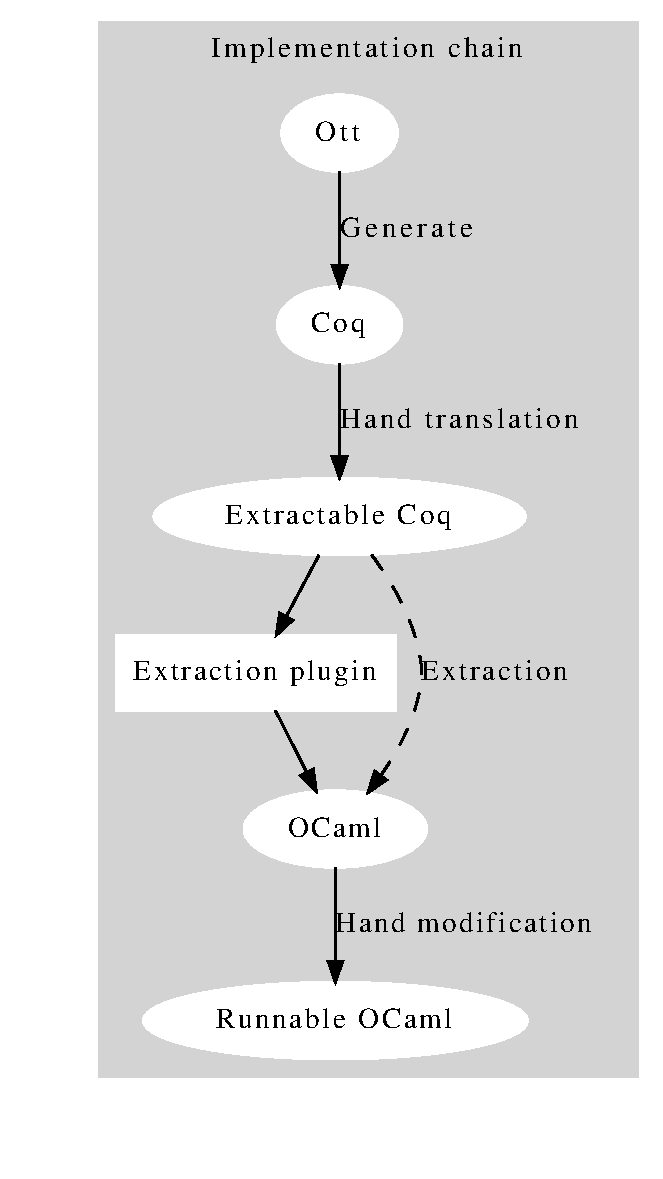
\includegraphics[scale=0.5]{implOut}
\caption{Detailed outline of the implementation}
\label{fig:detailedimploutline}
\end{center}
\end{figure}


The overall semantics were defined in Ott. These semantics were then extracted to Coq by Ott in a logical inductive format. This format, as previously mentioned, is well suited for proofs, but not for extraction. 

I modified the logical inductive format of the semantics in the Extractable Coq stage to have a well formed input for the extraction plugin. This plugin will be detailed in \Cref{sec:extractable_plugin_descr}. After the extraction the generated OCaml is not yet runnable: it contains a number of placeholders necessary for logic model of the language, but not usable for computation. I replace these placeholders with the actual computations and provide some syntactic sugar.
\section{The semantics}\label{sec:the-semanticssec:the-semantics}
In this section I describe the implemented semantics. These semantics were written in Ott.  Much of the inspiration for the semantics of basic features comes from Benjamin C. Pierce: \textit{Types and Programming Languages}\cite{pierce2002types}. The Ott code was based on the simply typed $ \lambda $-calculus. For a \LaTeX\, version of the full semantics as produced by Ott see \cref{chap:fullsemantics}.

 
The semantics splits into three main parts
\begin{enumerate}
\item{Grammars:\begin{itemize}
\item{expressions, denoted by $ e $}
\item{values, denoted by $ v $}
\end{itemize}}
\item{Types and type judgements}
\item{Reduction judgements}
\end{enumerate}

I detail the semantics in two groups of features: basic features that form a standard extension to the simply typed $ \lambda $-calculus and the monadic concurrency features. The basic features are arrow types or functions, sum types or tagged unions, product types or pairs and the fixpoint combinator. The monadic concurrency features are the monadic primitives and the fork operator. The presentation of semantics for the features was inspired by Pierce\cite{pierce2002types}. Each feature group is presented by first examining the syntax and typing rules of the features followed by their operational semantics. In the syntax parts I introduce every new syntactic form used in the evaluation and typing rules, but I do not repeat previously mentioned syntax. The presentation of both the syntax and the evaluation and typing rules were slightly simplified for better readability.   
\subsection{Basic features: arrow, sum and product types, fixpoint}

\subsubsection{Arrow types}

\begin{figure}[h]
  \centering
  $\underbracket{\overbracket{\textrm{
  \begin{tabular}{l | l}
    \begin{minipage}{0.45\linewidth}
    \begin{tabularx}{\textwidth}{l l >{\raggedleft}X}
    \textit{Syntax} &  & \tabularnewline
    e\, ::=  &  & \textit{terms:}\tabularnewline
      & x  & \textit{value name}\tabularnewline
      & $ \lambda $x:T.e  & \textit{abstraction}\tabularnewline
      & e e  & \textit{application}\tabularnewline
      &   & \tabularnewline
      v\, ::=  &  & \textit{values:}\tabularnewline
      & $ \lambda $x:T.e  & \textit{abstraction value}\tabularnewline
      &   & \tabularnewline
      T\, ::=  &  & \textit{types:}\tabularnewline
      & T$ \rightarrow $T  & $ \rightarrow $ \textit{type}\tabularnewline
      &   & \tabularnewline
      $ \Gamma $\, ::=  &  & \textit{contexts:}\tabularnewline
      & $ \emptyset $  & \textit{empty context}\tabularnewline
      & $ \Gamma,  $ x:T  & \textit{term variable binding}\tabularnewline 
    \end{tabularx}
    \end{minipage} & \begin{minipage}{0.45\linewidth}
        \begin{tabular}{l}
        \begin{minipage}{\textwidth}
           \begin{tabularx}{\textwidth}{>{\raggedright}X}
                        \textit{Typing} \hfill \fbox{$ \Gamma\, \vdash \, $t : T}  \tabularnewline   \begin{equation}
                        \inferrule
                          { \textrm{x:T}\in\, \Gamma}
                          { \Gamma\, \vdash \, \textrm{x : T}} \tag{T-Var}
                        \end{equation} \vspace{-9mm}
                        \tabularnewline   \begin{equation}
                         \inferrule
                          { \Gamma \, \vdash \, e \, : \, T_1\rightarrow T_2 \\\\ 
                            \Gamma \, \vdash \, e' \, : \, T_1}
                          { \Gamma\, \vdash \, e\,e' \, :\, T_2} \tag{T-App}
                          \end{equation}\vspace{-9mm}
                        \tabularnewline   \begin{equation}
                        \inferrule
                        { \Gamma, x : T_1 \, \vdash \, e \, : \, T_2}
                        { \Gamma\, \vdash \, \lambda\, x\,:\,T_1. e \, :\, T_1 \rightarrow T_2}\label{eq:t_fun} \tag{T-Fun}
                                                  \end{equation}\vspace{-5mm}
                      \end{tabularx}
        \end{minipage}
        \end{tabular}
        \end{minipage} 
    \end{tabular}
}}}$
  \caption{Syntax and typing of arrow types}
  \label{fig:syntyparrow}
\end{figure}




Arrow types or functions are ubiquitous in functional programming languages. In \Cref{fig:syntyparrow} I detail the basic syntax and typing of functions in a simply typed setting, while \Cref{fig:evalarrow} shows the operational semantics. The style and details are based on Pierce\cite[p.~103]{pierce2002types}. A function abstraction $ \lambda x:T. e $ encloses a yet unreduced expression $ e $ that may involve the variable $ x $ that is bound by the abstraction. 


\subsubsection{Sum types}

\begin{figure}[h]
  \centering
  $\underbracket{\overbracket{\textrm{
  \begin{tabular}{l | l}
    \begin{minipage}[t][][t]{0.37\linewidth}
    \begin{tabularx}{\textwidth}{l l >{\raggedleft}X}
    \textit{Syntax} &  & \tabularnewline
    e\, ::=  &  & \textit{terms:}\tabularnewline
       $\textbf{left}\, e$ & & \textit{left}\tabularnewline
       $\textbf{right}\, e$ & & \textit{right}\tabularnewline
       Case $ e_1 $ of  &  & \textit{case}\tabularnewline
       \hspace{9pt} \textbf{left} $ x_1 \Rightarrow e_2 $   &  & \tabularnewline
       \hspace{3pt} \vline \, \textbf{right} $ x_2 \Rightarrow e_3 $  &  & \tabularnewline
      &   & \tabularnewline
      v\, ::=  &  & \textit{values:}\tabularnewline
       $\textbf{left}\, v$ & & \textit{left}\tabularnewline
       $\textbf{right}\, v$ & & \textit{right}\tabularnewline
      &   & \tabularnewline
      T\, ::=  &  & \textit{types:}\tabularnewline
       $ T+T $  & &  \textit{sum type}\tabularnewline
    \end{tabularx} 
    \end{minipage} & \begin{minipage}{0.65\linewidth}
        \begin{tabular}{l}
        \begin{minipage}{\textwidth}
           \begin{tabularx}{\textwidth}{>{\raggedright}X}
                        \textit{Typing} \hfill \fbox{$ \Gamma\, \vdash \, $t : T}  \tabularnewline   \begin{equation}
                        \inferrule
                          { \Gamma\, \vdash \, \, e\, :\, T_1}
                          { \Gamma\, \vdash \, \textbf{left} \, e\, :\, T_1 + T_2} \tag{T-Left}
                        \end{equation} \vspace{-5mm}
                        \tabularnewline   \begin{equation}
                         \inferrule
                          { \Gamma\, \vdash \, \, e\, :\, T_2}
                          { \Gamma\, \vdash \, \textbf{right} \, e\, :\, T_1 + T_2} \tag{T-Right}
                          \end{equation}\vspace{-5mm}
                        \tabularnewline   \begin{equation}
                        \inferrule
                        { \Gamma\, \vdash \, \, e\, :\, T_1 + T_2 \\\\ \Gamma,x_1:T_1\, \vdash \, \, e_2\, :\, T \\\\ \Gamma,x_2:T_2\, \vdash \, \, e_3\, :\, T}
                        { \Gamma\, \vdash \, (\textrm{Case $  e $ of \textbf{left} $ x_1 \Rightarrow e_2 $ \vline\, \textbf{right} $ x_2 \Rightarrow e_3 $ })\, :\, T} \tag{T-Case}
                                                  \end{equation}\vspace{-5mm}
                      \end{tabularx}
        \end{minipage}
        \end{tabular}
        \end{minipage} 
    \end{tabular}
}}}$
  \caption{Syntax and typing of sum types}
  \label{fig:semsyntype}
\end{figure}


Many circumstances require the ability to describe expressions that are either one type or the other. Sum types or otherwise known as labelled unions are a simple solution to this. An expression $ e $ that has type $ T $ can be labelled as a variant in a sum type by attaching a label $ \textbf{left } e $ and $ \textbf{right } e $ will give force it to have type $ T + T' $ and $ T' + T $ for some type $ T' $. This expression can be then destructed by the expression "$ \textrm{Case $  e $ of \textbf{left} $ x_1 \Rightarrow e_2 $ \vline\, \textbf{right} $ x_2 \Rightarrow e_3 $ } $" which will evaluate to either a substitution of $ e_2 $ or $ e_3 $ depending on what the tag said. In this project I use sum types in the signature of \textbf{fork} that will be detailed in \Cref{sec:fork_sem}. \Cref{fig:semsyntype} shows basic structure of sum types that is based on Pierce\cite[p.~132]{pierce2002types}. I chose not to use the slightly more complex version of sum types offered by Pierce that would ensure unique typing. Simplicity had a higher priority than typing properties, however further work should include a change to the uniquely typable variant. 


\subsubsection{Product types}
One very common feature of functional languages is pairs or product types. Grouping different types of data together in one logical unit often makes code more simple. For example computations with complex numbers would be rather unintuitive if we always had to handle the real and imaginary parts separately. To define products, first I introduce the syntax $ \{e, e' \} $, the pair of expressions $ e $ and $ e' $. If they had types $ T $ and $ T' $ respectively I define the type construct for this $ T\star T' $. I introduced three primitive functions to deal with pairs: \textbf{pair} places two values in a pair, \textbf{proj1} takes the first element of a pair and \textbf{proj2} takes the second.

\begin{figure}[h]
  \centering
  $\underbracket{\overbracket{\textrm{
  \begin{tabular}{l | l}
    \begin{minipage}{0.45\linewidth}
     \begin{tabular}{l}
    \begin{tabularx}{\textwidth}{l l >{\raggedleft}X}
    \textit{Syntax} &  & \tabularnewline
    e\, ::=  &  & \textit{terms:}\tabularnewline
      & $\{e,e'\}$  & \textit{pair}\tabularnewline
      & $\textbf{pair}\,e\, e'$  & \textit{to pair}\tabularnewline
      & $\textbf{proj}_1\,e$  & \textit{first projection}\tabularnewline
      & $\textbf{proj}_2\,e$  & \textit{second projection}\tabularnewline
      &   & \tabularnewline
      v\, ::=  &  & \textit{values:}\tabularnewline
      & $\{v,v'\}$  & \textit{pair}\tabularnewline
      &   & \tabularnewline
      T\, ::=  &  & \textit{types:}\tabularnewline
      & $T\star T$  & \textit{product type}\tabularnewline 
    \end{tabularx}  
        \end{tabular}
        \end{minipage} & \begin{minipage}{0.55\linewidth}
        \begin{tabular}{l}
        \begin{minipage}{\textwidth} 
                           \begin{tabularx}{\textwidth}{>{\raggedright}X}
                                        \textit{Typing} \hfill \fbox{$ \Gamma\, \vdash \, $t : T}  \tabularnewline   \begin{equation}
                                        \inferrule
                                          { \Gamma\, \vdash \, e\,:\, T_1 \\ \Gamma\, \vdash \, e'\,:\, T_2}
                                          { \Gamma\, \vdash \, \{e,\,e'\}\,:\, T_1\star T_2} \tag{T-Pair}
                                        \end{equation} \vspace{-7mm}
                                        \tabularnewline   \begin{equation}
                                         \inferrule
                                          { \Gamma\, \vdash \, e \, :\,  T_1 \\\\  \Gamma\, \vdash \,e' \, :\,  T_2}
                                          { \Gamma\, \vdash \, \textbf{pair}\,e\,e' \, :\,  T_1\star T_2} \tag{T-InPair}
                                          \end{equation}\vspace{-7mm}
                                        \tabularnewline
                                        \begin{equation}
                                          \inferrule
                                          { \Gamma\, \vdash \, e \, :\,  T_1\star T_2}
                                          { \Gamma\, \vdash \, \textbf{proj}_1\,e \, :\,  T_1} \tag{T-Proj1}
                                          \end{equation}\vspace{-7mm}
                                                                \tabularnewline
                                          \begin{equation}
                                          \inferrule
                                          {\Gamma\, \vdash \, e \, :\,  T_1\star T_2}
                                          { \Gamma\, \vdash \, \textbf{proj}_2\,e \, :\, T_2} \tag{T-Proj2}
                                                                    \end{equation}
                                      \end{tabularx}
                        \end{minipage}
        \end{tabular}
        \end{minipage} 
    \end{tabular}
}}}$
  \caption{Syntax and typing of product types}
  \label{fig:syntypprod}
\end{figure}


\Cref{fig:syntypprod} shows the syntax and typing rules of product types defined in this language. The style and details are based on Pierce\cite[p.~126]{pierce2002types}.
\subsubsection{Fixpoint combinator}

\begin{figure}[h]
  \centering
  $\underbracket{\overbracket{\textrm{
  \begin{tabular}{l | l}
    \begin{minipage}{0.5\linewidth}
    \begin{tabularx}{\textwidth}{l l >{\raggedleft}X}
    \textit{Syntax} &  & \tabularnewline
    e\, ::=  &  & \textit{terms:}\tabularnewline
      & $\textbf{fix}\, e$  & \textit{fixpoint}\tabularnewline
    \end{tabularx}
    \end{minipage} & \begin{minipage}{0.50\linewidth}
        \begin{tabular}{l}
        \begin{minipage}{\textwidth}
           \begin{tabularx}{\textwidth}{>{\raggedright}X}
                        \textit{Typing} \hfill \fbox{$ \Gamma\, \vdash \, $t : T}  \tabularnewline    \begin{equation}
                        \inferrule
                        {\Gamma\, \vdash \, e\, :\, T \rightarrow T}
                        { \Gamma\, \vdash \, \textbf{fix}\,e\, :\,  T} \label{eq:t_fix} \tag{T-Fix}
                                                  \end{equation}\vspace{-5mm}
                      \end{tabularx}
        \end{minipage}
        \end{tabular}
        \end{minipage} 
    \end{tabular}
}}}$
  \caption{Syntax and typing of the fixpoint operator}
  \label{fig:semfix}
\end{figure}


Recursion is very characteristic of functional programming languages. There are many ways to achieve recursive constructs in terms and even in types. A very elegant treatment surfaced from the formal study of recursive constructs with the syntax and typing properties show in \Cref{fig:semfix}. It is important to note that because of \Cref{eq:t_fix} all types have at least one term in them: 
\begin{equation}
                        \inferrule
                        {\Gamma\, \vdash \, \lambda\, x\, :\, T. \, x\, :\, T \rightarrow T}
                        { \Gamma\, \vdash \, \textbf{fix}\,(\lambda\, x\, :\, T. \, x)\, :\,  T} \label{eq:t_all} \tag{T-All}
                                                  \end{equation}
The assumption of \Cref{eq:t_all} is always true because of \Cref{eq:t_fun} in \Cref{fig:syntyparrow}.


\subsubsection{Operational semantics of the basic MOCaml features}

The reduction semantics of MOCaml is given as small step labelled transitions. Small step semantics means that the reduction relation between two expressions $ e, \, e' $ means that $ e $ can directly and atomically transition to $ e' $. Labelled transitions further extend this idea. In this project I used a 4-tuple $ (e, s, rl, e') $ of the starting expression, a selection operator that will be supplied by a scheduler to pick between potential reductions, a reduction label that describes the observable action and the ending expression of the transition. This 4-tuple means that given the selection operator, which may be 1 or 2, a starting expression $ e $  can move to $ e' $ with a side-effect $ rl $. I use the notation $ e \overset{rl}{\underset{s}{\longrightarrow}} e' $. The $ rl $ label may be $ \tau $ which is a silent action or an atomic action $ e $ that can be observed. A silent action $tau$ is considered unobservable from outside MOCaml. The atomic action $e$ is in fact considered an expression within the model.  This choice was based on the behaviour of placeholders in \Cref{sec:comp_place_syn}. The inspiration to use a labelled transition system to model side-effects comes from Milner's ``A calculus of communicating systems" book\cite{milner1982calculus}.



% Fun opsem

\begin{figure}[H]
  \centering
  $\underbracket{\overbracket{\textrm{
  \begin{tabular}{l | l}
    \begin{minipage}{0.4\linewidth}
    \begin{tabularx}{\textwidth}{l l >{\raggedleft}X}
    \textit{Syntax} &  & \tabularnewline
      $ rl $\, ::=  &  & \textit{labels:}\tabularnewline
      & $ \tau $  & \textit{silent}\tabularnewline
      & $ e $  & \textit{action}\tabularnewline
      &   & \tabularnewline
      $ s $\, ::=  &  & \textit{select:}\tabularnewline
      & $ 1 $  & \textit{first}\tabularnewline
      & $ 2 $  & \textit{second}\tabularnewline      
    \end{tabularx}
    \end{minipage} & \begin{minipage}{0.50\linewidth}
        \begin{tabular}{l}
        \begin{minipage}{\textwidth}
         \begin{tabularx}{\textwidth}{>{\raggedright}X}
             \textit{Evaluation} \hfill \fbox{$e \, \overset{rl}{\underset{s}{\longrightarrow}} \, e'$}  \tabularnewline   \begin{equation}
                                     \inferrule
                                       {  }
                                       { ( \lambda\, x\,:\,T. e)\, v \overset{\tau}{\underset{s}{\longrightarrow}} \{v / x\}e } \tag{R-Subst}
                                     \end{equation} \vspace{-9mm}
                                     \tabularnewline   \begin{equation}
                                      \inferrule
                                       { e \overset{rl}{\underset{s}{\longrightarrow}} e''}
                                       { e\,e' \, \overset{rl}{\underset{s}{\longrightarrow}}\, e''\, e'\,  } \tag{R-App1}
                                       \end{equation}\vspace{-9mm}
                                     \tabularnewline   \begin{equation}
                                     \inferrule
                                      { e' \overset{rl}{\underset{s}{\longrightarrow}} e''}
                                      { v\,e' \, \overset{rl}{\underset{s}{\longrightarrow}}\, v\, e''\,  } \tag{R-App2}
                                                               \end{equation}
             \end{tabularx}
        \end{minipage}
        \end{tabular}
        \end{minipage} 
    \end{tabular}
}}}$
  \caption{Syntax of the reduction relation and operational semantics of arrow types}
  \label{fig:evalarrow}
\end{figure}


\Cref{fig:evalarrow} shows the transition rules for functions and applications. I used call-by-value semantics for functions and left-first reduction. Furthermore, arguments are explicitly annotated in functions and substitution does not provide facilities for renaming. The lack of renaming is a trade-off between logical simplicity and ease of use and I chose to keep the logical model as simple as possible. It is presumed that the user of the framework takes care of picking fresh variable names, but I provided facilities with the syntactic sugar to pick fresh variables. \label{sec:subst_caveat}

% Sum opsem
\begin{figure}[H]
  \centering
  $\underbracket{\overbracket{\textrm{
   \begin{minipage}{\textwidth}
            \begin{tabularx}{\textwidth}{>{\raggedright}X}
                \textit{Evaluation} \hfill \fbox{$e \, \overset{rl}{\underset{s}{\longrightarrow}} \, e'$}  \tabularnewline   \begin{equation}
                        \inferrule
                                                       { e \overset{rl}{\underset{s}{\longrightarrow}} e' }
                                                       { (\textrm{Case $  e $ of \textbf{left} $ x_1 \Rightarrow e_2 $ \vline\, \textbf{right} $ x_2 \Rightarrow e_3 $ }) \\\\ \overset{rl}{\underset{s}{\longrightarrow}} \\\\
                                                       (\textrm{Case $  e' $ of \textbf{left} $ x_1 \Rightarrow e_2 $ \vline\, \textbf{right} $ x_2 \Rightarrow e_3 $ }) } \tag{R-Case}
                                                     \end{equation} \vspace{-7mm}
                                                     \tabularnewline 
                           \begin{equation}
                                        \inferrule
                                          {  }
                                          { (\textrm{Case $  \textbf{left}\, v $ of \textbf{left} $ x_1 \Rightarrow e_2 $ \vline\, \textbf{right} $ x_2 \Rightarrow e_3 $ }) \overset{\tau}{\underset{s}{\longrightarrow}} \{v / x_1\}e_2 } \tag{R-CaseL}
                                        \end{equation}  \vspace{-7mm}
                                        \tabularnewline \begin{equation}
                                            \inferrule
                                            {  }
                                            { (\textrm{Case $  \textbf{right}\, v $ of \textbf{left} $ x_1 \Rightarrow e_2 $ \vline\, \textbf{right} $ x_2 \Rightarrow e_3 $ }) \overset{\tau}{\underset{s}{\longrightarrow}} \{v / x_2\}e_3 } \tag{R-CaseR}
                                                                             \end{equation} \vspace{-7mm}
                                                                             \tabularnewline
                                           \begin{equation}
                                         \inferrule
                                          { e \overset{rl}{\underset{s}{\longrightarrow}} e'}
                                          { \textbf{left}\,e \, \overset{rl}{\underset{s}{\longrightarrow}}\, \textbf{left}\,e'\,  } \tag{R-Left}
                                          \end{equation}\vspace{-7mm}
                                        \tabularnewline   \begin{equation}
                                        \inferrule
                                         { e \overset{rl}{\underset{s}{\longrightarrow}} e'}
                                         { \textbf{right}\,e \, \overset{rl}{\underset{s}{\longrightarrow}}\, \textbf{right}\,e'\,  } \tag{R-Right}
                                                                  \end{equation}
                \end{tabularx}
           \end{minipage}
}}}$
  \caption{Operational semantics of sum types}
  \label{fig:semeval}
\end{figure}

In \Cref{fig:semeval} I describe the transition rules for constructs related to sum types: the destructor Case and the constructors \textbf{left} and \textbf{right}. This can be used to dynamically use some behaviour information and signal within MOCaml without the need to include the complexity of redefining constructs like if and tests. The not capture avoiding substitution may cause an issue for the user in this case as well.


% Pair opsem
\begin{figure}[H]
  \centering
  $\underbracket{\overbracket{\textrm{
  \begin{tabular}{l  l}
    \begin{minipage}{0.5\linewidth}
     \begin{tabular}{l}
    \begin{tabularx}{\textwidth}{>{\raggedright}X}
     \textit{Evaluation} \hfill \fbox{$e \, \overset{rl}{\underset{s}{\longrightarrow}} \, e'$}  \tabularnewline   \begin{equation}
                                         \inferrule
                                           { e \overset{rl}{\underset{s}{\longrightarrow}} e''}
                                           { \{e,e'\} \overset{rl}{\underset{s}{\longrightarrow}} \{e'',e'\} } \tag{R-Pair1}
                                         \end{equation} \vspace{-5mm}
                                         \tabularnewline
                                         \begin{equation}
                                           \inferrule
                                             { e' \overset{rl}{\underset{s}{\longrightarrow}} e''}
                                             { \{v,e'\} \overset{rl}{\underset{s}{\longrightarrow}} \{v,e''\} } \tag{R-Pair2}
                                             \end{equation} \vspace{-5mm}
                                                                              \tabularnewline
                                            \begin{equation}
                                          \inferrule
                                           {}
                                           { \textbf{pair}\,v\,v' \, \overset{\tau}{\underset{s}{\longrightarrow}}\, \{v, v'\}  } \tag{R-InPair}
                                           \end{equation}\vspace{-7mm}
                                         \tabularnewline
                                          \begin{equation}
                                           \inferrule
                                           {e \overset{rl}{\underset{s}{\longrightarrow}} e''}
                                          { \textbf{pair}\,e\,e' \, \overset{rl}{\underset{s}{\longrightarrow}}\,\textbf{pair}\,e''\,e' \,  } \tag{R-InPair-Eval1}
                                                                                \end{equation}\vspace{-7mm}
    \end{tabularx} 
    \end{tabular}
    \end{minipage} & \begin{minipage}{0.50\linewidth}
        \begin{tabular}{l}
        \begin{minipage}{\textwidth}
         \begin{tabularx}{\textwidth}{>{\raggedright}X}
                                     \begin{equation}
                                     \inferrule
                                     {e' \overset{rl}{\underset{s}{\longrightarrow}} e''}
                                     { \textbf{pair}\,v\,e' \, \overset{rl}{\underset{s}{\longrightarrow}}\,\textbf{pair}\,v\,e'' \,  } \tag{R-InPair-Eval2}
                                     \end{equation}\vspace{-7mm}
                                     \tabularnewline
                                     \begin{equation}
                                       \inferrule
                                         {}
                                         { \textbf{proj}_1\,\{v,\,\,v'\} \, \overset{\tau}{\underset{s}{\longrightarrow}}\, v  } \tag{R-Proj1}
                                      \end{equation}\vspace{-7mm}
                                     \tabularnewline
                                     \begin{equation}
                                       \inferrule
                                       { e \overset{rl}{\underset{s}{\longrightarrow}} e'}
                                       { \textbf{proj}_1\,e \, \overset{rl}{\underset{s}{\longrightarrow}}\, \textbf{proj}_1\,e  } \tag{R-Proj1-Eval}
                                       \end{equation}\vspace{-7mm}
                                                     \tabularnewline
                                     \begin{equation}
                                      \inferrule
                                      {}
                                      { \textbf{proj2}\,\{v,\,\,v'\} \, \overset{\tau}{\underset{s}{\longrightarrow}}\, v'  } \tag{R-Proj2}
                                                                           \end{equation}
                                      \vspace{-7mm}
                                     \tabularnewline
                                     \begin{equation}
                                     \inferrule
                                    { e \overset{rl}{\underset{s}{\longrightarrow}} e'}
                                    { \textbf{proj}_2\,e \, \overset{rl}{\underset{s}{\longrightarrow}}\, \textbf{proj}_2\,e  } \tag{R-Proj2-Eval}
                                                                             \end{equation}
             \end{tabularx}
        \end{minipage} 
        \end{tabular}
        \end{minipage} 
    \end{tabular}
}}}$
  \caption{Operational semantics of product types}
  \label{fig:evalprod}
\end{figure}

\Cref{fig:evalprod} details the operational semantics of pairs, the constructor \textbf{pair} and destructors $ \textbf{proj}_1 $ and $ \textbf{proj}_2 $. These semantics mimic the implementation by Pierce. In a previous iteration of these primitives I provided them curried, that is to say available for partial application. However, Ott did not handle the partial application correctly with respect to the value subgrammar, therefore I hand modified the generated Coq script. The new semantics actually provide a way to offer partially applied counterparts to these primitives: 
\[ \lambda\, x\, :\, T.\lambda\,y\,:\,T'.\textbf{pair}\,\,x\,\,y   \]
The above expression has equivalent behaviour to a curried \textbf{pair} primitive.

% Fixpoint opsem

\begin{figure}[H]
  \centering
  $\underbracket{\overbracket{\textrm{
  \begin{minipage}{\textwidth}
           \begin{tabularx}{\textwidth}{>{\raggedright}X}
               \textit{Evaluation} \hfill \fbox{$e \, \overset{rl}{\underset{s}{\longrightarrow}} \, e'$}  \tabularnewline    \begin{equation}
                                       \inferrule
                                        {}
                                        { \textbf{fix}\,(\lambda x:T. e) \, \overset{\tau}{\underset{s}{\longrightarrow}}\, \{(\textbf{fix}\,(\lambda x:T. e))/x \}e  } \tag{R-Fix}
                                                                 \end{equation} \vspace{-7mm}
              \tabularnewline    \begin{equation}
               \inferrule
                {e \overset{rl}{\underset{s}{\longrightarrow}} e'}
                { \textbf{fix}\,e \, \overset{rl}{\underset{s}{\longrightarrow}}\, \textbf{fix}\,e'   } \tag{R-Fix-Eval}
                                                                             \end{equation} 
               \end{tabularx}
          \end{minipage}
}}}$
  \caption{Operational semantics of the fixpoint operator}
  \label{fig:evalfix}
\end{figure}

In denotational semantics loops and other recursions are treated as the greatest fixpoints of continuous functions. A fixpoint combinator $ y $ is defined as a term that given a function $ f $ satisfies
\[ y\,f\,\equiv\, f\,(y\,f) \] 
This axiom poses a requirement on the type of $ y $: it should be $ (T \rightarrow T) \rightarrow T $ which is the type in \Cref{fig:semfix}. I return to the exact notion of equivalence in \Cref{sec:behave_equiv} for theoretical evaluation.
In untyped $ \lambda $-calculus there are many simple terms that can achieve this, for example the Y combinator:
\[ Y = \lambda f.(\lambda x.f\ (x\ x))\ (\lambda x.f\ (x\ x))  \]
However in strict, call-by-value languages like MOCaml arguments are always reduced before the function application can begin. In this setting the Y combinator would always diverge. There a few implementation options in call-by-value languages, but I have chosen to use the one described in Pierce\cite[p.~144]{pierce2002types}. This style fits well with the tool chain I used as it does not require a partial function application that Ott sometimes handles incorrectly with respect to the value subgrammar.
\clearpage

\subsection{Extensions: computation place holders, monadic primitives and fork}
The standard features described in the previous section form the basis on which I built the primitives for monadic concurrency. In this section I first describe the syntax and types of the primitives and then move on to operational details.
\subsubsection{Computation place holders}
\label{sec:comp_place_syn}
\begin{figure}[h!]
  \centering
  $\underbracket{\overbracket{\textrm{
  \begin{tabular}{l | l}
    \begin{minipage}{0.5\linewidth}
    \begin{tabularx}{\textwidth}{l l >{\raggedleft}X}
    \textit{Syntax} &  & \tabularnewline
    e\, ::=  &  & \textit{terms:}\tabularnewline
      & comp e  & \textit{computation}\tabularnewline
    \end{tabularx}
    \end{minipage} & \begin{minipage}{0.50\linewidth}
        \begin{tabular}{l}
        \begin{minipage}{\textwidth}
           \begin{tabularx}{\textwidth}{>{\raggedright}X}
                        \textit{Typing} \hfill \fbox{$ \Gamma\, \vdash \, $t : T}  \tabularnewline      \begin{equation}
                         \inferrule
                          { \Gamma \, \vdash \, e \, : \,  T}
                          {\Gamma \, \vdash \,\text{comp } e \, : \,  T} \tag{T-Comp}
                          \end{equation}
                      \end{tabularx}
        \end{minipage}
        \end{tabular}
        \end{minipage} 
    \end{tabular}
}}}$
  \caption{Syntax and typing of the computation place holder}
  \label{fig:syntypcomp}
\end{figure}

In previous subsections there were no constructs that accept external computations. Without such a construct MOCaml would not behave as a framework for concurrency, but just as an exercise in semantics. In \Cref{fig:syntypcomp} I introduce a new expression called a computation place holder. These are the holes that will be filled by actual OCaml $ \textbf{unit} \rightarrow \text{expr} $ functions to be evaluated. 

\subsubsection{Monadic primitives}

\begin{figure}
  \centering
  $\underbracket{\overbracket{\textrm{
  \begin{tabular}{l | l}
    \begin{minipage}{0.5\linewidth}
    \begin{tabularx}{\textwidth}{l l >{\raggedleft}X}
    \textit{Syntax} &  & \tabularnewline
    e\, ::=  &  & \textit{terms:}\tabularnewline
      & Live e  & \textit{live expression}\tabularnewline
      & ()  & \textit{unit}\tabularnewline
      & \textbf{ret}\,e  & \textit{return}\tabularnewline
      & e $\gg=$ e'  & \textit{bind}\tabularnewline
      &   & \tabularnewline
      v\, ::=  &  & \textit{values:}\tabularnewline
      & Live e  & \textit{live expression}\tabularnewline
      & ()  & \textit{unit}\tabularnewline
      &   & \tabularnewline
      T\, ::=  &  & \textit{types:}\tabularnewline
      & \textbf{con}\,T  & \textit{concurrent}\tabularnewline
       & \textbf{unit}  & \textit{unit}\tabularnewline
    \end{tabularx}
    \end{minipage} & \begin{minipage}{0.50\linewidth}
        \begin{tabular}{l}
        \begin{minipage}{\textwidth}
           \begin{tabularx}{\textwidth}{>{\raggedright}X}
                        \textit{Typing} \hfill \fbox{$ \Gamma\, \vdash \, $t : T}  \tabularnewline      \begin{equation}
                         \inferrule
                          { \Gamma \, \vdash \, e \, : \, \textbf{con } T_1 \\\\ 
                            \Gamma \, \vdash \, e' \, : \, T_1 \rightarrow \textbf{con } T_2}
                          { \Gamma\, \vdash \, e\, \gg= \,e' \, :\, \textbf{con } T_2} \tag{T-Bind}
                          \end{equation}\vspace{-9mm}
                        \tabularnewline
                        \begin{equation}
                        \inferrule
                        {\Gamma\, \vdash \, \, e \, :\, T}
                        { \Gamma\, \vdash \, \textbf{ret }\, e \, :\, \textbf{con } T} \tag{T-Ret}
                                                                          \end{equation}\vspace{-9mm}
                                                 \tabularnewline 
                          \begin{equation}
                         \inferrule
                         {\Gamma\, \vdash \, \, e \, :\, T}
                         { \Gamma\, \vdash \, \textit{Live } \, e \, :\, \textbf{con }T} \tag{T-LiveExpr}
                         \end{equation}\vspace{-9mm}
                         \tabularnewline
                         \begin{equation}
                         \inferrule
                         {}
                         { \Gamma\, \vdash \, () \, :\, \textbf{unit }} \tag{T-Unit}
                                                  \end{equation}\vspace{-5mm}
                      \end{tabularx}
        \end{minipage}
        \end{tabular}
        \end{minipage} 
    \end{tabular}
}}}$
  \caption{Syntax and typing of the monadic primitives, ret and bind}
  \label{fig:syntypmon}
\end{figure}

 The concurrency monad consists of a parametric type $  \textbf{con } T  $, where $ T $ is a type parameter describing the type of computation or value enclosed and three key operations. 
\begin{itemize}
\item{ret, also known as return. From the monadic axioms, mentioned in \Cref{sec:monad_first_mention}, it follows that it has type $ T \rightarrow \textbf{con }T   $ as shown in \Cref{fig:syntypmon}}
\item{$\gg=$, also known as bind, sequences two operations. The second argument is the continuation for the first parameter. More formally it has a type $ \textbf{con } T_1  \rightarrow ( T_1 \rightarrow \textbf{con } T_2 ) \rightarrow \textbf{con } T_2  $. Bind takes a boxed up computation and a function that takes the value of the computation and returns a new box.}
\end{itemize}

\textit{Live} is a tag attached to boxed up expressions, much like \textbf{inl} for sum types.  

\subsubsection{Fork}
\label{sec:fork_sem}
\begin{figure}[h]
  \centering
  $\underbracket{\overbracket{\textrm{
  \begin{tabular}{l | l}
    \begin{minipage}{0.35\linewidth}
                \begin{tabularx}{\linewidth}{l l >{\raggedleft}X}
                        \textit{Syntax} &  & \tabularnewline
                        e\, ::=  &  & \textit{terms:}\tabularnewline
                          & \textbf{fork}\,\,e\,\,e'  & \textit{fork}\tabularnewline
                        \end{tabularx}
            \end{minipage} & \begin{minipage}{0.6\linewidth}
        \begin{tabular}{l} 
        \begin{minipage}{\linewidth}
           \begin{tabularx}{\textwidth}{>{\raggedright}X}
                        \textit{Typing} \hfill \fbox{$ \Gamma\, \vdash \, $t : T}  \tabularnewline   \begin{equation}
                        \inferrule
                          { \Gamma\, \vdash \, e \, :\, \textbf{con } T_1 \\\\ \Gamma\, \vdash \, e \, : \, T_1\, \rightarrow\,\textbf{con } T_2  }
                          { \Gamma\, \vdash \,\textbf{fork}\,\,e\,\,e' \, :  \, \\\\ \textbf{con } ((T_1\star \textbf{con } T_2)+((\textbf{con }T_1)\star  T_2)} \tag{T-Fork}
                        \end{equation} \vspace{-5mm}
                      \end{tabularx}
        \end{minipage}
        \end{tabular}
        \end{minipage} 
    \end{tabular}
}}}$
  \caption{Syntax and typing of the fork operator}
  \label{fig:semfork}
\end{figure}

Up until this point I have not mentioned any language feature that implements concurrency which is the main focus of the dissertation. The third, additional operation of the concurrency monad is fork, which is the way to spawn new threads (two in this particular case). There are a number of ways to implement fork and indeed this project went through various iterations of semantics for this operation. 

As a first approximation I had to decide on the signature of fork. On the argument side fork may take zero, one, two or many arguments. No arguments would be reminiscent of the UNIX system call \verb|fork()| where the two paths are distinguished by replacing the fork call with differing values. This approach would result in copying potentially large expressions and a more complex evaluation context, that is the terms used for the source and destination in the reduction relation. For example, Jones\cite{hoareetal2001tackling} chose an implementation with one argument, however with a similar requirement of a metalanguage of parallel terms $ e \, | \, e' $. I chose to go with two arguments as that can maintain a simple evaluation context with reductions from language expression to expression. The choice between these three argument styles is largely arbitrary as they all implicitly form the binary parallel composition $ e \, | \, e' $. Note however that several arguments can be elegantly simulated by composing binary parallel compositions.

To stay within the monad I decided to have the arguments as already boxed terms, that is of type $ \textbf{con } T_1 $ and $ \textbf{con } T_2 $ for some $ T_1, T_2 $. For better expressibility, I chose not to take the two arguments curried. As seen previously currying is possible by two function abstractions, therefore for simplicity, I describe  \textbf{fork} as a higher-order function: given the first argument it returns a function that takes only one parameter and will then behave as the parallel composition. This gives the following signature:

\[ \textbf{fork} \, : \, \textbf{con } T_1 \rightarrow \, (\textbf{con } T_2\, \rightarrow\, R ) \tag{T-Fork1} \]  

where $ R $ is the yet not described return type. Currying allows partial application of \textbf{fork} and to be passed around as a value with only one edge filled. 

To keep within the monad, I required that $ R $ be a concurrent type, that is $ R =  \textbf{con } R' $ for some $ R' $ type. There are many choices available for the return type. Other popular concurrency primitives have varying return semantics. For example \textbf{join} would return the pair of values resulted from the two expressions giving $ R = \textbf{con }(T_1 \star T_2) $. Another primitive, \textbf{choose} would pick one and discard the other: $ R = \textbf{con }(T_1 + T_2) $. I wanted to provide a combination of this: to signal which thread has finished first, but keep the partially reduced other edge around, so the user can use it. From the previous constructions a return type as $ R = \textbf{con }((T_1\star \textbf{con } T_2) + ((\textbf{con } T_1) \star T_2)) $ would implement this behaviour. At first glance, this seems to be a rather complex signature but  it is versatile enough to implement both other \textbf{join} and \textbf{choose} and capture the semantics of a wide range of problems well. The return type also raises the question of interleaving semantics: as I am implementing concurrency in software I was not constrained by hardware to interleave reductions. It would be perfectly acceptable to reduce both edges of a fork at the same time if possible. Indeed this project was originally designed with not necessarily interleaving semantics in mind. However, that lead to a blow up in the number of rules, the complexity of signature ($ R = \textbf{con }((T_1\star \textbf{con } T_2) + ((\textbf{con } T_1) \star T_2) + (T_1 \star T_2))   $) and the number of potential behaviours of the system. I chose to simplify to interleaving semantics for the theoretical simplicity over potential efficiency gains.

Putting this all together gives the full signature of \textbf{fork} as 
\[ \textbf{fork} \, : \, \textbf{con } T_1 \rightarrow \, (\textbf{con } T_2\, \rightarrow\, \textbf{con }((T_1\star \textbf{con } T_2) + ((\textbf{con } T_1) \star T_2)) ) \] 
This corresponds to the type shown in \Cref{fig:semfork}.

\subsubsection{The operational semantics of the MOCaml concurrency features}

% Comp place opsem
\label{sec:comp_place_sem}
\begin{figure}[h!]
  \centering
  $\underbracket{\overbracket{\textrm{
 \begin{minipage}{\textwidth}
          \begin{tabularx}{\textwidth}{>{\raggedright}X}
              \textit{Evaluation} \hfill \fbox{$e \, \overset{rl}{\underset{s}{\longrightarrow}} \, e'$}  \tabularnewline    \begin{equation}
                                       \inferrule
                                        {}
                                        { \textbf{comp }\,e \, \overset{e}{\underset{s}{\longrightarrow}}\,  e } \tag{R-DoComp}
                                        \end{equation}\vspace{-7mm}
              \end{tabularx}
         \end{minipage}
}}}$
  \caption{Operational semantics of the computation placeholder}
  \label{fig:evalcomp}
\end{figure}

\Cref{fig:evalcomp} shows the reduction rule for a computation place holder. It may be unintuitive but that is because it only exists in this form in the logical model: the place holder will be fully replaced by a call to an OCaml function that returns an expression. The purpose of the expression within the place holder is purely logical: it serves as a tool to prove that the sequence of actual code calls obey certain properties. 

I chose to always reduce a place holder to an expression within the framework to provide an easy way for flexible, dynamic behaviour. This also means that the typing statement in \Cref{fig:syntypcomp} is not enforced: it is assumed that the user pays attention to the return expression type. Future work could include a way to type check expressions and to modify the extracted OCaml to enforce this typing rule.

% Monprim opsem
\begin{figure}[H]
  \centering
  $\underbracket{\overbracket{\textrm{
 \begin{minipage}{\textwidth}
          \begin{tabularx}{\textwidth}{>{\raggedright}X}
              \textit{Evaluation} \hfill \fbox{$e \, \overset{rl}{\underset{s}{\longrightarrow}} \, e'$}  \tabularnewline    \begin{equation}
                                       \inferrule
                                        {}
                                        { \textbf{ret }\,v \, \overset{\tau}{\underset{s}{\longrightarrow}}\, \textit{Live } v } \tag{R-Return}
                                        \end{equation}\vspace{-7mm}
                                        \tabularnewline    \begin{equation}
                                        \inferrule
                                         { e \overset{rl}{\underset{s}{\longrightarrow}} e'}
                                        { \textbf{ret }\,e \, \overset{rl}{\underset{s}{\longrightarrow}}\, \textbf{ret }\,e } \tag{R-Evalret}
                                                                                \end{equation}\vspace{-7mm}
                                      \tabularnewline   \begin{equation}
                                      \inferrule
                                       { e \overset{rl}{\underset{s}{\longrightarrow}} e''}
                                       { e\,\gg=\,e' \, \overset{rl}{\underset{s}{\longrightarrow}}\, e''\, \gg= e'\,  } \tag{R-Evalbind}
                                                                \end{equation}\vspace{-9mm}
                                      \tabularnewline   
                                      \begin{equation}
                                       \inferrule
                                       { e \overset{rl}{\underset{s}{\longrightarrow}} e''}
                                       { \textit{Live }  e\,\gg=\,e' \, \overset{rl}{\underset{s}{\longrightarrow}}\, \textit{Live } e''\, \gg= e'\,  } \tag{R-Movebind}
                                                                                                     \end{equation}\vspace{-9mm}
                                                                           \tabularnewline
                                      \begin{equation}
                                      \inferrule
                                      {}
                                      { \textit{Live }  v\,\gg=\,e' \, \overset{\tau}{\underset{s}{\longrightarrow}}\, e'\, v  } \tag{R-Dobind}                                                                                                                              \end{equation}\vspace{-7mm}
              \end{tabularx}
         \end{minipage}
}}}$
  \caption{Operational semantics of the monadic primitives, ret and bind}
  \label{fig:evalmon}
\end{figure}

\Cref{fig:evalmon} shows the semantics of the concurrent type constructor \textbf{ret} and the operation \textbf{bind}. The \textbf{ret} operation first reduces its argument to a value and then boxes it up as a concurrent value. 


Bind evaluates left to right: it evalutes the expression on the left to a concurrent box, reduces the internal expression of the box and then passes it to the expression on the right. This fits well with the idea of sequencing operations: any side effect $ e' $ might have happens after the side effects of $ e $.
% Fork opsem

\begin{figure}
  \centering
  $\underbracket{\overbracket{\textrm{
  \begin{tabular}{l}
    \begin{minipage}{\linewidth}
     \begin{tabularx}{\textwidth}{>{\raggedright}X}
                 \textit{Evaluation} \hfill \fbox{$e \, \overset{rl}{\underset{s}{\longrightarrow}} \, e'$}  \tabularnewline   \begin{equation}
                                         \inferrule
                                           {e \overset{rl}{\underset{s}{\longrightarrow}} e'' \\ e' \notin \text{Values} }
                                           { \textbf{fork } (\textit{Live } e) (\textit{Live } e')  \overset{rl}{\underset{1}{\longrightarrow}} \textbf{fork } (\textit{Live } e'') (\textit{Live } e')  } \tag{R-Forkmove1} \label{eq:forkmove1}
                                         \end{equation} \vspace{-7mm}
                                         \tabularnewline   \begin{equation}
                                          \inferrule
                                            {e' \overset{rl}{\underset{s}{\longrightarrow}} e'' \\ e \notin \text{Values} }
                                            { \textbf{fork } (\textit{Live } e) (\textit{Live } e') \overset{rl}{\underset{2}{\longrightarrow}} \textbf{fork }  (\textit{Live } e) (\textit{Live } e'')  } \tag{R-Forkmove2} \label{eq:forkmove2}
                                           \end{equation}\vspace{-7mm}\tabularnewline
                                            \begin{equation}
                                            \inferrule
                                            {}
                                            { \textbf{fork } (\textit{Live } v) (\textit{Live } e')  \overset{\tau}{\underset{1}{\longrightarrow}} \textit{Live } \textbf{left}  \{v, (\textit{Live } e')\}  } \tag{R-Forkdeath1}   \end{equation} \vspace{-7mm} \tabularnewline
                          \begin{equation}
                                                                      \inferrule
                                                                      {}
                         { \textbf{fork } (\textit{Live } e) (\textit{Live } v')  \overset{\tau}{\underset{2}{\longrightarrow}} \textit{Live } \textbf{right}  \{(\textit{Live }e) ,  v'\}  } \tag{R-Forkdeath2}   \end{equation} \vspace{-7mm}\tabularnewline\begin{equation}\inferrule{e \overset{rl}{\underset{s}{\longrightarrow}} e'' }{ \textbf{fork }\,\,  e\,\, e'  \overset{rl}{\underset{s}{\longrightarrow}} \textbf{fork } \,\, e'' \,\, e' } \tag{R-Forkeval1} \label{eq:forkeval1}\end{equation}\vspace{-7mm}
                        \tabularnewline\begin{equation}\inferrule{e' \overset{rl}{\underset{s}{\longrightarrow}} e'' }{ \textbf{fork }\,\,  v\,\, e'  \overset{rl}{\underset{s}{\longrightarrow}} \textbf{fork } \,\, v \,\, e'' } \tag{R-Forkeval2} \label{eq:forkeval2}\end{equation}   
                 \end{tabularx}
    \end{minipage}
    \end{tabular}
}}}$
  \caption{Operational semantics of the fork operator}
  \label{fig:evalfork}
\end{figure}

In \Cref{fig:evalfork} I give the detailed operational semantics of fork. Notice that this is the first time the selection operator of the reduction relation is explicitly specified. A selection value of 1 will try to reduce the first edge of the fork, a value of 2 will try to reduce the second edge. When either edge contains a value the \textbf{fork} is forced to return to the respective tagged value, regardless of the selection value. This gives a finer grade of control for the user to choose what to do with the other edge, however it increases overhead as value checks always have to be carried out on both edges.   \clearpage
\section{Proof assisstant system}
In this section I briefly outline the structure of the translated proof assistant representation and how I modified it to be extractable to OCaml. 
\subsection{Outline of the proof assistant code}

There are four types of objects in the Coq semantics:
\begin{enumerate}
\item{Inductive sets: they are the inductive data structures. These were translated from expression grammar objects. As an example, type expressions were translated from the Ott version in \Cref{lst:otttypexpr} to the Coq equivalent in \Cref{lst:coqtypexpr}. Simple grammars generate a set of tagged variants. 

\begin{lstlisting}[language={Ott}, caption={Ott type expressions}, label={lst:otttypexpr}]
typexpr, t :: TE_ ::=
  | tunit                           ::   :: unit
  | typexpr -> typexpr'                ::   :: arrow
  | typexpr '*' typexpr'               ::   :: prod
  | con typexpr                        ::   :: concurrent
  | typexpr '+' typexpr'               ::   :: sum
  | ( typexpr )                        :: S :: paren {{ ich [[typexpr]] }} {{ ocaml [[typexpr]] }}
\end{lstlisting}


\begin{minipage}{\linewidth}

\begin{lstlisting}[language={Coq},caption={Coq type expr}, label={lst:coqtypexpr}]
Inductive typexpr : Set := 
 | TE_unit : typexpr
 | TE_arrow (typexpr5:typexpr) (typexpr':typexpr)
 | TE_prod (typexpr5:typexpr) (typexpr':typexpr)
 | TE_concurrent (typexpr5:typexpr)
 | TE_sum (typexpr5:typexpr) (typexpr':typexpr).
\end{lstlisting}

\end{minipage}
}
\item{Fixpoints, the functions in Coq: The functions in this are all automatically generated from the Ott file. The most important ones are the expression substitution, free variable, value check fixpoints. The script also includes a few functions supporting the previous ones. The value subgrammar shown in \Cref{lst:ottvaluesub} was translated to the fixpoint in \Cref{lst:coqvaluesub}. 

\begin{minipage}{\linewidth}
\begin{lstlisting}[language={Ott}, caption={Ott value subgrammar}, label={lst:ottvaluesub}]
value, v :: V_ ::=
  | unit                           ::   :: unit
  | function value_name : typexpr -> expr        ::   :: function
  | live e                         ::   :: live_expr
  | inl v                              ::   :: taggedleft
  | inr v                              ::   :: taggedright
  | { v , v' }                         ::   :: valuepair
  | ( v )                             :: S :: paren {{ ich [[v]] }} {{ ocaml [[v]] }}
\end{lstlisting}
\end{minipage}


\begin{minipage}{\linewidth}
\begin{lstlisting}[language={Coq},caption={Coq value subgrammar}, label={lst:coqvaluesub}, escapeinside={@}{@}]
Fixpoint is_value_of_expr (e_5:expr) : Prop :=
  match e_5 with
  | (E_ident value_name5) => False
  | E_unit => (True)
  | (E_apply expr5 expr') => False
  | (E_bind expr5 expr') => False
  | (E_function value_name5 t e) => (True)
  | (E_fix e) => False
  | (E_comp e) => False
  | (E_live_expr e) => (True)
  | (E_pair e e') => ((is_value_of_expr e) /\ (is_value_of_expr e'))
  | (E_inpair e e') => False
  | (E_proj1 e) => False
  | (E_proj2 e) => False
  | (E_fork e e') => False
  | (E_ret e) => False
  | (E_taggingleft e) => ((is_value_of_expr e))
  | (E_taggingright e) => ((is_value_of_expr e))
  | (E_case e1 x1 e2 x2 e3) => False
end.
\end{lstlisting}

\end{minipage}	
Ott offers single and multiple substitution predicates for its destination languages. These are implemented as fixpoints in Coq. As an example, see the expression substitution in \Cref{lst:coqexprsubst}.
\begin{minipage}{\linewidth}

\begin{lstlisting}[language={Coq},caption={Coq expression substitution}, label={lst:coqexprsubst}]
Fixpoint subst_expr (e_5:expr) (x_5:value_name) (e__6:expr) {struct e__6} : expr :=
  match e__6 with
  | (E_ident value_name5) => (if eq_value_name value_name5 x_5 then e_5 else (E_ident value_name5))
  | E_unit => E_unit 
  | (E_apply expr5 expr') => E_apply (subst_expr e_5 x_5 expr5) (subst_expr e_5 x_5 expr')
  ...
end
\end{lstlisting}

\end{minipage}	
}
\item{Logical inductive sets: As mentioned previously a logical inductive set is an inductively defined set of propositions. The reduction relation and the typing relation were represented with a logical inductive set. For example a clause in the reduction relation was translated from the simple inference rule presentation in \Cref{lst:ottcontextapp1} to a proposition in the logical inductive set \verb|JO_red| in \Cref{lst:coqlogind}.


\begin{lstlisting}[language={Ott}, caption={Ott reduction relation example}, label={lst:ottcontextapp1}]
e [ s ] --> [ rl ] e''
----------------------------  :: context_app1
e e' [ s ] --> [ rl ] e'' e'
\end{lstlisting}


\begin{minipage}{\linewidth}

\begin{lstlisting}[language={Coq},caption={Coq reduction relation example}, label={lst:coqlogind}]
Inductive JO_red : expr -> select -> redlabel -> expr -> Prop :=    (* defn red *)
 | JO_red_context_app1 : forall (e e':expr) (s:select) (rl:redlabel) (e'':expr),
     JO_red e s rl e'' ->
     JO_red (E_apply e e') s rl (E_apply e'' e')
  ...
\end{lstlisting}

\end{minipage}	
}
\item{Lemmas: There is a supporting lemma about the equality of variables. This was automatically generated by Ott as shown in \Cref{lst:coqeqlabel}.
\begin{minipage}{\linewidth}

\begin{lstlisting}[language={Coq},caption={Coq variable equality lemma}, label={lst:coqeqlabel}]
Lemma eq_value_name: forall (x y : value_name), {x = y} + {x <> y}.
Proof.
  decide equality; auto with ott_coq_equality arith.
Defined.
\end{lstlisting}

\end{minipage}	

}
\end{enumerate} 
\subsection{Extractable reduction relation}
As I mentioned in \Cref{sec:first_mention_logind}, Coq provides extraction facilities to OCaml and Haskell, but not from inductive sets and fixpoints that involve propositions, more specifically the \textit{Prop} sort. 

Logical inductive types are often used as descriptions of various concepts in semantics, especially reduction relations. Ott generates a logical inductive relation as seen in \Cref{lst:coqlogind}. For simple relations, like the value relation in \Cref{lst:coqvaluesub} it is simple to rewrite in a set inductive manner. However, for complex non-terminating relations, like the reduction relation in this project, rewriting is not feasible.  Delahaye et al.\cite{delahaye2007extracting,tollitte2012producing} proposed a method of extracting such relations to OCaml by annotating the input/output modes of the elements of the relation. \label{sec:extractable_plugin_descr}

I rewrote the value check logical fixpoint to an extractable version by simply replacing the True and False propositions by their boolean counterpart and successfully extracted it by the built-in Coq extraction. However, not even the Coq plugin based on element modes could extract the reduction relation generated by Ott. 

The first issue with the extraction to a functional program was the way the selection argument was supplied. Originally, the reduction relation only required a single selection value. In the case of fork reduction rules in \Cref{eq:forkmove1ex,eq:forkmove2ex} this would not be enough to generate a certified program.

\begin{equation}
\inferrule
{e \overset{rl}{\underset{s}{\longrightarrow}} e'' \\ e' \notin \text{Values} }
{ \textbf{fork } (\textit{Live } e) (\textit{Live } e')  \overset{rl}{\underset{1}{\longrightarrow}} \textbf{fork } (\textit{Live } e'') (\textit{Live } e')  } \tag{R-Forkmove1} \label{eq:forkmove1ex}
\end{equation}
\begin{equation}
\inferrule
{e' \overset{rl}{\underset{s}{\longrightarrow}} e'' \\ e \notin \text{Values} }
 { \textbf{fork } (\textit{Live } e) (\textit{Live } e') \overset{rl}{\underset{2}{\longrightarrow}} \textbf{fork }  (\textit{Live } e) (\textit{Live } e'')  } \tag{R-Forkmove2} \label{eq:forkmove2ex}
                                           \end{equation}

The extracted program would have to somehow pick a possible value for $ s $ in $ e \overset{rl}{\underset{s}{\longrightarrow}} e' $ while it is only supplied with the value 1. Always picking one or the other would not be satisfactory. As I had no way of choosing it non-deterministically, I wanted the argument to fully describe all $ s $ values the system used. I opted for a co-inductive stream of selections because there can be an arbitrary number of \textbf{fork}s nested in each other with arbitrary number of selection values necessary to make a single step. \vspace{5mm}

\begin{minipage}{\linewidth}

\begin{lstlisting}[language={Coq},caption={Coq co-inductive selection sequence}, label={lst:coqselectstar}]
CoInductive selectstar : Set := Seq : select -> selectstar -> selectstar.
\end{lstlisting}

\end{minipage}

Co-inductive data structures represent potentially infinite data and featured in a number of programming languages: lazy lists, trees and streams all describe co-inductive structures. In \Cref{lst:coqselectstar} I define \verb|selectstar| where each element is pair of a selection value and a further \verb|selectstar| representing the rest of the selection values.  With an infinite sequence of selection values the program can make arbitrary many decisions and it is extractable.

The second problem that surfaced was that the extraction plugin does not generate code that backtracks from a case where the reduction relation is invoked on an internal part. If an expression $ e $ does not reduce and the extracted function is called it will fail with an \lstinline|assert false|. I chose to add a logically superfluous assumption of expression $ e $ not being a value. This assumption is superfluous as an expression that reduces cannot be a value by the \verb|red_not_value| theorem.  \Cref{lst:coqredunsafe,lst:coqxredsafe} are a good example of how this transformation happens. \vspace{4mm}

\begin{minipage}{0.9\linewidth}

\begin{lstlisting}[language={Coq},caption={Coq reduction clause with unsafe assumption}, label={lst:coqredunsafe}]
| JO_red_evalbind : forall (e e'':expr) (s:select) (rl:redlabel) (e':expr),
     JO_red e s rl e' ->
     JO_red (E_bind e e'') s rl (E_bind e' e'')
\end{lstlisting}

\end{minipage}

\begin{minipage}{\linewidth}

\begin{lstlisting}[language={Coq},caption={Coq extractable reduction clause with safe assumption}, label={lst:coqxredsafe}]
 | XJO_red_evalbind : forall (e e'' e':expr) (s:selectstar),
    (eq (xis_value_of_expr e) false) ->
     XJO_red e s e' ->
     XJO_red (E_bind e e'') s (E_bind e' e'')
\end{lstlisting}

\end{minipage}


The last issue was due to the experimental nature of the plugin: the optimisations and inference algorithm ran out of stack space when invoked with all 31 rules. Therefore I extracted in three parts and recombined them by hand.

\section{OCaml system}
In this section I give a brief outline of the structure of the extracted OCaml, how it is modified to be runnable and a brief overview of potential syntactic sugar that can be used to aid development in the framework. 

\subsection{Outline of the OCaml code}
The OCaml code consists of the extracted versions of the following:
\begin{itemize}
\item{Inductive sets like expressions, constants and type expressions as tagged variants or type constructors.}
\item{Functions like the expression substitution or xJO\_red12, the single step reduction function.}
\item{The metavariables \verb|value_name ident| are both OCaml \lstinline|int|s instead of constructor based extractions of Coq \lstinline[language={Coq}]|nat|. This has the caveat that \lstinline|int| may overflow or represent negative numbers, while the Coq \lstinline[language={Coq}]|nat| cannot. Realistically, no program would have this problem.}
\end{itemize}
\subsection{Hand modifications and justifications}
I have made a number of modifications to the OCaml code to make it runnable. This includes changing the type of labels from int to $ (\textbf{unit}\rightarrow\text{expr}) $ and inserting terms in the relevant cases to run these computations. 

Furthermore I have changed the way \verb|selectstar| is implemented. The extraction results in the type in \Cref{lst:ocamllazystar} which involves the Lazy module of OCaml. While the extraction of co-inductive types to lazy types is sound, for simplicity I used a simple lazy stream in \Cref{lst:ocamlstreamstar}. 


\vspace{3mm}
\begin{minipage}{\linewidth}

\begin{lstlisting}[caption={OCaml lazy selectstar}, label={lst:ocamllazystar}]
type selectstar = __selectstar Lazy.t
and __selectstar =
| Seq of select * selectstar
\end{lstlisting}

\end{minipage}

\begin{minipage}{\linewidth}

\begin{lstlisting}[caption={OCaml stream selectstar}, label={lst:ocamlstreamstar}]
type selectstar = | Seq of select * (unit -> selectstar) 
\end{lstlisting}

\end{minipage}

As the extraction plugin is experimental there were a number of inefficiencies and a few issues due to the fact that the semantics of OCaml pattern matching is sequential, while it is parallel in Coq. While Tollitte\cite{tollitte2012producing} made progress on the merging of cases when one case subsumes the other, these were not always correctly identified. For example the case in \Crefrange{lst:ocamlvalexpappcaseStart}{lst:ocamlvalexpappcaseEnd} in \Cref{lst:ocamlorigapp} subsumes the case in \Cref{lst:ocamlorigsub}. The plugin was unable to infer this as that would have required it to show that function term is always a value, regardless of its parameters. This is an issue as any function with a parameter that can be reduced will fail, as the case in \Cref{lst:ocamlorigsub} comes first.


\vspace{3mm}

\begin{minipage}{\linewidth}

\begin{lstlisting}[caption={OCaml original substitution case}, label={lst:ocamlorigsub}]
  | (E_apply (E_function (x, t, e), v), s) ->
    (match xis_value_of_expr v with
     | true -> subst_expr v x e
     | _ -> assert false (*  *))
\end{lstlisting}

\end{minipage}

\begin{minipage}{\linewidth}

\begin{lstlisting}[caption={OCaml original application case}, label={lst:ocamlorigapp}, escapeinside={@}{@}]
  | (E_apply (e, e'), s) ->
    (match xis_value_of_expr e with
     | false ->
 @\label{lst:ocamlunneededmatchonfun}@      (match xJO_red12 e s with
        | e'' -> E_apply (e'', e')
        | _ -> assert false (*  *))
 @\label{lst:ocamlvalexpappcaseStart}@    | true ->
       (match xJO_red12 e' s with
        | e'' -> E_apply (e, e'')
 @\label{lst:ocamlvalexpappcaseEnd}@       | _ -> assert false (*  *))
 @\label{lst:ocamlunneededdefault2}@    | _ -> assert false (*  *))
\end{lstlisting}

\end{minipage}
My solution was to insert the correct step into the failing match as in \Cref{lst:ocamlfixsub}. Note, that taking that reduction may fail, but that is the expected behaviour.


\vspace{3mm}
\begin{minipage}{\linewidth}

\begin{lstlisting}[caption={OCaml fixed substitution case}, label={lst:ocamlfixsub}]
  | (E_apply (E_function (x, t, e), v), s) ->
    (match xis_value_of_expr v with
     | true -> subst_expr v x e
     | false -> E_apply (E_function (x, t, e), (xJO_red12 v s)))
\end{lstlisting}

\end{minipage}
A reoccurring inefficiency comes from the extraction plugin generating a default failing case in all situations, even if the default case may never happen. \Cref{lst:ocamlunneededdefault2} in \Cref{lst:ocamlorigapp} is an example of this: a boolean may only take the values true or false. A similar issue occurs when evaluating a function:  \Cref{lst:ocamlunneededmatchonfun} in the same listing matches by giving a name to the return value, but generates a default case as well. I simply removed the superfluous match and replaced the name of the return value with the function call.

A further issue occurs when occasionally the plugin reorders matches on assumptions. Even though the safe assumption was inserted in the case in \Cref{lst:ocamlswapassume} it was reordered by the plugin to come after the unsafe assumption.\vspace{2mm}

\begin{minipage}{\linewidth}
\begin{lstlisting}[caption={OCaml swapped assumptions}, label={lst:ocamlswapassume}]
  | (E_bind (e, e''), s) ->
    (match xJO_red12 e s with
     | e' ->
       (match xis_value_of_expr e with
        | false -> E_bind (e', e'')
        | _ -> assert false (*  *))
     | _ -> assert false (*  *))
\end{lstlisting}

\end{minipage}
The simple solution to this is to swap the assumptions, however in some cases that leads to to the issues mentioned above.
\subsection{Syntactic sugar}
Due to the multiple layers of automatic naming developing in this framework directly could be cumbersome. I have defined a few OCaml functions to serve as syntactic sugar. The two broad categories of sugar are syntax to build expressions and schedulers. 
\begin{itemize}
\item{Boxing expressions and computations: \lstinline|let boxe e = E_live_expr e|, \lstinline|let boxc f = E_live_expr (E_comp f)|}
\item{An infix bind operator: \lstinline|let ( >>= ) a b = E_bind (a, b)|}
\item{Application: \lstinline|let app a b = E_apply (a, b)|}
\item{Fork: \lstinline|let fork a b = E_fork (a, b)|}
\item{Round-robin and random schedulers in \Cref{lst:ocamlrrsched} and \Cref{lst:ocamlrandsched} respectively.}
\end{itemize}
\begin{minipage}{\linewidth}

\begin{lstlisting}[caption={OCaml round-robin scheduler}, label={lst:ocamlrrsched}]
  let rec makerr1 () = Seq(S_First, makerr2) 
  and makerr2 () = Seq(S_Second, makerr1) 
  
  let rec evalrr1 e n = (match n with 
           | 0 -> e
           | m -> evalrr2 (xJO_red12 e (makerr1 ())) (m-1))
  and evalrr2 e n = (match n with 
           | 0 -> e
           | m -> evalrr1 (xJO_red12 e (makerr2 ())) (m-1))
\end{lstlisting}

\end{minipage}
\begin{minipage}{\linewidth}

\begin{lstlisting}[caption={OCaml random scheduler}, label={lst:ocamlrandsched}]
  let rec makerand () = if Random.bool() then Seq(S_First, makerand) else Seq(S_Second, makerand)
  
  let rec evalrand e n = (match n with 
                       | 0 -> e
                       | m -> evalrand (xJO_red12 e (makerand ())) (m-1))
\end{lstlisting}

\end{minipage}


\cleardoublepage
\chapter{Evaluation}
In this chapter I evaluate the implementation from two perspectives: theoretical and performance. The theoretical evaluation examines the implementation 


\section{Theoretical evaluation}
\label{sec:behave_equiv}
There are a number of properties that are expected from this system: monadic laws, process calculus axioms and potentially properties of the fixpoint operator, predicates for pairs, type preservation and progress. These requirements are all phrased as equivalences as mentioned in \Cref{sec:first_mention_of_equiv}. 

First the semantics of the equivalence $ \equiv $ had to be examined. If two expressions are equivalent they should behave the same: for an outside observer there has to be no difference which exact expression is evaluated in a black box computation. One way to capture this is by keeping track of potential effects and side-effects. Effects are the return values of an expression, side-effects are the computation placeholders invoked by the system. That is why I phrased the operational semantics with labelled transitions: the labels are descriptions of the side-effects.

Labelled transition systems, like the operational semantics I have defined, is a common way to describe systems with side-effects. As the selection operator is external and not determined by the system I consider it and therefore the transition system non-deterministic. Brookes\cite{brookes1983behavioural} surveys various equivalence relations over non-deterministic labelled transitions systems. I chose to follow Milner\cite{milner1982calculus} and use weak bisimilarity with a slight modification.

\subsection{Weak bisimilarity}
Bisimilarity is a standard method for establishing behavioural equivalence of a non-deterministic language used by Milner for CCS\cite{milner1982calculus}, Pierce and Sangiorgi for $ \pi $-calculus\cite{pierce2000behavioral} and Bergstra for the Algebra of Communicating Processes\cite{bergstra1986algebra,bergstra1985algebra} among others. 

In the following definitions I use $ p,\, q,\, e $ as expressions, $ \alpha $ as an atomic action, $ \tau $ as a silent action, $ \delta $ as an action that may be either silent or atomic and $ p \overset{\delta}{\rightarrow} p' $ as the statement that for some selection value $ p $ may transition in a single step to $ p' $ with a side-effect $ \delta $.

\begin{defn}
Two expressions $ p $ and $ q $ are \textit{bisimilar} if and only if
\begin{itemize}
\item{For all $ q' $ such that $ q \overset{\delta}{\rightarrow} q' $ there is a $ p' $ such that $ p \overset{\delta}{\rightarrow} p' $ and $ p' $ and $ q' $ are bisimilar. }
\item{For all $ p' $ such that $ p \overset{\delta}{\rightarrow} p' $ there is a $ q' $ such that $ q \overset{\delta}{\rightarrow} q' $ and $ p' $ and $ q' $ are bisimilar. }
\end{itemize}
\end{defn}

Weak bisimilarity is an extension to bisimilarity by noting that in some cases not all reductions need to be observable: Milner\cite{milner1982calculus} introduces $ \tau $ or silent reductions that do not have observable effects. In this setting it would be unnecessarily restrictive to require that two expression simulate the unobservable behaviour of each other. 

\begin{defn}
$ p $ \textit{silently reduces} to $ p' $ or $ p \overset{\tau}{\Rightarrow} p' $ if and only if $ (p, p') \in \left(\overset{\tau}{\rightarrow}\right)^* $, that is, the two expressions are in the transitive, reflexive closure of $ \overset{\tau}{\rightarrow} $. More simply if $ p $ can reduce to $ p' $ with zero or more $ \tau $ steps.
\end{defn}

\begin{defn}
$ p $ \textit{weakly reduces} to $ p' $ with side-effect $ \delta $ or $ p \overset{\delta}{\Rightarrow} p' $ if and only if 
\begin{itemize}
\item{in the case $ \delta = \tau $, $ p \overset{\tau}{\Rightarrow} p' $}
\item{in the case $ \delta = \alpha $, there exist $ p_1, p_2 $ expressions such that $ p \overset{\tau}{\Rightarrow} p_1 $, $ p_1 \overset{\alpha}{\rightarrow} p_2 $, $ p_2 \overset{\tau}{\Rightarrow} p' $}
\end{itemize}
\end{defn}

A simplified version of Milner's definition for weak bisimilarity states:
\begin{defn}[Milner]
A relation $ \mathcal{R} $ between expressions is a \textit{weak bisimulation} if and only if for all expressions $ p $ and $ q $ such that $ (p,q)\in \mathcal{R} $ or $ p\, \mathcal{R}\, q $:
\begin{itemize}
\item{For all $ q' $ such that $ q \overset{\delta}{\Rightarrow} q' $ there is a $ p' $ such that $ p \overset{\delta}{\Rightarrow} p' $. and $ (p', q') \in \mathcal{R}$. }
\item{For all $ p' $ such that $ p \overset{\delta}{\Rightarrow} p' $ there is a $ q' $ such that $ q \overset{\delta}{\Rightarrow} q' $. and $ (p', q') \in \mathcal{R}$. }
\end{itemize}
\end{defn}

Sangiorgi\cite{sangiorgi1992problem} remarks that there is an equivalent definition that is much easier to show:
\begin{defn}[Sangiorgi]
A relation $ \mathcal{R} $ between expressions is a \textit{weak bisimulation} if and only if for all expressions $ p $ and $ q $ such that $ (p,q)\in \mathcal{R} $ or $ p\, \mathcal{R}\, q $:
\begin{itemize}
\item{For all $ q' $ such that $ q \overset{\delta}{\rightarrow} q' $ there is a $ p' $ such that $ p \overset{\delta}{\Rightarrow} p' $. and $ (p', q') \in \mathcal{R}$. }
\item{For all $ p' $ such that $ p \overset{\delta}{\rightarrow} p' $ there is a $ q' $ such that $ q \overset{\delta}{\Rightarrow} q' $. and $ (p', q') \in \mathcal{R}$. }
\end{itemize}
\end{defn}

I proved this equivalence for the transition system of MOCaml. This second definition is much easier to show in Coq as Coq generates an inversion lemma for a single step however not for a weak reduction. Weak bisimulation has a number of useful properties: if $ \mathcal{R} $ and $ \mathcal{S} $ are weak bisimulations then $ \mathcal{R}^{-1}, \mathcal{R}^*, \mathcal{R}^+, \mathcal{R}\cup\mathcal{S}$  and $\mathcal{R} \circ \mathcal{S} $ are all weak bisimulations.
\begin{defn}
\label{defn:weak_bisimilarity}
Two expressions $ p $ and $ q $ are \textit{weakly bisimilar} or $ p\approx q $ if there is a weak bisimulation $ \mathcal{R} $ such that $ (p,q) \in \mathcal{R} $.
\end{defn}

\Cref{defn:weak_bisimilarity} is equivalent to saying that weak bisimilarity $ \approx  $ is the union of all weak bisimulations. Weak bisimilarity is an equivalence relation: it is reflexive, symmetric and transitive.

While weak bisimilarity perfectly captures side-effect behaviour it does not capture equality of return values: all values are weakly bisimilar as values do not reduce. Therefore in many cases I will use a restriction of weak bisimilarity:

\begin{defn}
\label{defn:ve_weak_bisim}
A weak bisimulation $ \mathcal{R} $ is \textit{value equal} if for all $ v, v' $ values if $ v\,\mathcal{R}\,v' $ then $ v = v' $
\end{defn}

\begin{defn}
\label{defn:ve_weak_bisimilarity}
Two expressions $ p $ and $ q $ are \textit{value equal weakly bisimilar} or $ p\approx_v q $ if there is a value equal weak bisimulation $ \mathcal{R} $ such that $ p\, \mathcal{R} \, q $.
\end{defn}

These definitions also enjoy the same properties as their non-restricted counterparts. All of these definitions and some supporting lemmas can be found in \verb|weakBisimulations.v|.
\subsection{Properties of the logical model}

In this section I introduce a number of properties that I required from the implementation and the way they apply. I give a slightly informal statement for each of these properties and a sketch of the major points in the proofs. \Cref{cha:full_proof_statements} gives the precise Coq statements of the theorems along with some supporting lemmas and structures. 

First, I describe the three monadic laws mentioned in \Cref{sec:monad_first_mention}. Then I attempt to show some of the basic process algebra axioms used by Bergstra for his Algebra of Communicating Processes\cite{bergstra1986algebra,bergstra1984process}. These properties can be summarized as follows:
\begin{align}
x + y &= y + x \label{eq:fork_comm}\\
(x + y) + z &= x + (y + z) \label{eq:fork_assoc}\\
x + x &= x \label{eq:choice_id}\\
(x + y)\cdot z &= (x \cdot z) + (y \cdot z) \label{eq:fork_bind_distribute}\\
(x \cdot y)\cdot z &= x \cdot (y \cdot z) \label{eq:bind_assoc}\\
\delta + x &= x \label{eq:fork_deadlock} \\
\delta \cdot x &= \delta \label{eq:bind_deadlock}
\end{align}

In the above axioms $ + $ denotes ``alternative composition" which resembles the \textbf{choose} operator. Sequential composition is denoted by $ \cdot $ and a process that cannot move forward, that is it is deadlocked is written as $ \delta $. 

By understanding $ + $ as the \textbf{fork} primitive of MOCaml only \Cref{eq:fork_comm,eq:fork_assoc,eq:fork_deadlock} may be true: because of the semantics of \textbf{fork} \Cref{eq:choice_id,eq:fork_bind_distribute} cannot be true as they may duplicate side-effects. Sequential composition or bind is denoted by $ \cdot $.

\subsubsection{Monadic laws}
The formal proofs of the following theorems about the monadic laws governing \textbf{ret} and bind $ \gg= $ can be found in \verb|mconbaseMonProofs.v|.

\begin{thm}[Return is left neutral to bind]
For all expressions $ e, f $, if $ f $ is a value then
\[ \textbf{ret } e\,\gg=\, f\quad \approx_v \quad f\,e \]
\end{thm}

The left neutrality has a caveat: it is only true if the function is a value. If this was not the case then the left hand side of the weak bisimilarity would first reduce $ f $ and then $ e $ which was a conscious decision: it felt unintuitive to reduce the later part of a sequencing first. 

\begin{thm}[Return is right neutral to bind]
For any value $ v$
\[  \textit{Live }v\,\gg=\, \textbf{ret}\quad \approx_v \quad \textit{Live }v \]
\end{thm}

\begin{thm}[Return is right neutral to bind, extended]
For any expression $ e$
\[  \textit{Live }e\,\gg=\, \textbf{ret}\quad \approx_v \quad \textbf{ret } e \]
\end{thm}

While the general statement of the right neutrality is 
\[  e\,\gg=\, \textbf{ret}\quad \approx_v \quad e \]
This is not true in general: if $ e $ reduces to a live expression that has an unreduced expression boxed the right hand side does not generate the side-effects of the boxed up computation. However, it is possible to show that in general if $ e $ always reduces to a boxed up value it will hold.

\begin{thm}[Bind is associative]
For any expression $ e $, values $ f, g $ and variable $ x $, if $ x $ appears neither in $ f $ nor in $ g $ either bound or free
\[ (e\, \gg=\, f) \, \gg=\, g \quad \approx_v \quad e\, \gg=\, (\lambda x. (f\, x) \, \gg=\, g ) \]
\end{thm}

This corresponds to \Cref{eq:bind_assoc} in Bergstra's axioms. The caveat mentioned about non-capture avoiding substitution in \Cref{sec:subst_caveat} appears in the associativity statement as well: $ x $ needs to be a fresh variable to avoid substitution to unintended variables.

\subsubsection{Fork commutativity}
The proofs of \textbf{fork} commutativity and associativity may be found in \verb|forkProofs.v|.

\begin{thm}[Fork commutative weak bisimilarity]
For all expressions $ e, e'$
\[  \textbf{fork}\,(\textit{Live }e)\,(\textit{Live }e')\quad \approx \quad \textbf{fork}\,(\textit{Live }e')\,(\textit{Live }e) \]
\end{thm}

Showing the weak bisimilarity of \textbf{fork} and the commuted version using Sangiorgi's definition of weak bisimilarity is very simple: for every step there is a corresponding single step of the respective expression in the commuted version. However the return values of the simply commuted \textbf{fork} are not equivalent to those of the original. I solved this by sequencing a function that ``swaps" the result:

\begin{thm}[Fork commutative value equal weak bisimilarity]
For all expressions $ e, e'$
\[  \textbf{fork}\,(\textit{Live }e)\,(\textit{Live }e')\quad \approx_v \quad (\textbf{fork}\,(\textit{Live }e')\,(\textit{Live }e))\gg=\text{swapf} \]
\end{thm}

\begin{lstlisting}[language={Coq}, caption={Swapf operator}, label={lst:swapf_op}]
Definition swapbodyl : expr :=
         E_ret (E_taggingright
            (E_inpair 
              (E_proj2  (E_ident (1))) 
              (E_proj1  (E_ident (1)))  
            )
     ).

Definition swapbodyr : expr :=
          E_ret (E_taggingleft  
            (E_inpair 
               (E_proj2  (E_ident (2))) 
               (E_proj1  (E_ident (2)))  
            )).

Definition swapbody : expr := E_case (E_ident (0)) 
           (1)  swapbodyl
           (2)  swapbodyr.

Definition swapf : expr :=
    E_function (0) TE_unit swapbody.
\end{lstlisting}
\Cref{lst:swapf_op} shows the definition of the swapf operator. It just swaps the output of the commuted fork to the correct return value. Notice that it does not obey the typing rule: to define swapf with correct type there has to be a family of swapf operators for each possible return type. By binding swapf onto the commuted \textbf{fork} we get a value equal weak bisimilarity as swapf is always silent.

\subsubsection{Fork associativity}
Fork in this implementation is not associative:

\begin{thm}[Fork is not associative]
There are expressions $a, b, c$
\[  \textbf{fork}\,(\textit{Live }(\textbf{fork}\,(\textit{Live }a)\,(\textit{Live }b)))\,(\textit{Live }c)\quad \not\approx \quad \textbf{fork}\,(\textit{Live }a)\,(\textit{Live }(\textbf{fork}\,(\textit{Live }b)\,(\textit{Live }c)) \]
\end{thm}

The example is:
\[ \textbf{fork } (\textit{Live }\textbf{fork }(\textit{Live }\textbf{unit})  (\textit{Live }\textbf{unit}))  (\textit{Live }\textit{comp } e) \tag{R-Assoc} \label{eq:fork_assoc_counter_r} \]
versus
\[ \textbf{fork } (\textit{Live }\textbf{unit})\,\,(\textit{Live }  \textbf{fork } ((\textit{Live }\textbf{unit})  (\textit{Live }\textit{comp } e))) \tag{L-Assoc} \label{eq:fork_assoc_counter_l} \]

While \ref{eq:fork_assoc_counter_r} may run the computation on the right, \ref{eq:fork_assoc_counter_l} can only return immediately as the left edge is a value. In the proof for this I used a computation that returns \textbf{unit}.
%\subsubsection{Join associativity}
%\begin{thm}[Join is associative]
%For all expressions $a, b, c$
%\[  \textbf{join}\,(\textit{Live }(\textbf{join}\,(\textit{Live }a)\,(\textit{Live }b)))\,(\textit{Live }c)\quad \approx \quad \textbf{join}\,(\textit{Live }a)\,(\textit{Live }(\textbf{join}\,(\textit{Live }b)\,(\textit{Live }c)) \]
%\end{thm}

\subsubsection{Deadlock properties}
The properties involving deadlock may be found in the file \verb|forkDeadlock.v|.

\begin{defn}
An expression $ \delta $ is \textit{deadlocked} if it can weakly reduce and any weak reduction it may make is silent and finishes in another \textit{deadlocked} expression. 
\end{defn}

This definition is closer to the common understanding of livelock, however as Bergstra\cite{bergstra1984process} explains: the ``action" taken by $ \delta $ is virtual, just acknowledging stagnation. This can occur by the incorrect use of the fixpoint combinator for example. In the proofs for the theorems below I used a stricter definition by only allowing deadlocked expressions that deterministically $ \tau $-step to themselves. In particular the example used to show that all types are occupied is a family of these expressions.
\begin{thm}[Fork deadlock]
For all expressions $ e, \delta$ if $ \delta $ is a deadlocked expression
\[  \textbf{fork}\,(\textit{Live }\delta)\,(\textit{Live }e)\quad \approx \quad e \]
\end{thm}

While the \textbf{fork} with a deadlocked edge is weakly bisimilar to the other edge, it has to be slightly modified to give value equality:

\begin{thm}[Fork deadlock value equivalence]
For all expressions $ e, \delta$ if $ \delta $ is a deadlocked expression
\[  (\textbf{fork}\,(\textit{Live }\delta)\,(\textit{Live }e))\gg=\text{takeright}\quad \approx_v \quad \textbf{ret }e \]
\end{thm}

\begin{lstlisting}[language={Coq}, caption={takeright operator}, label={lst:takeright_op}]
Definition takeright : expr :=
    E_function (0) TE_unit 
      (E_case (E_ident (0)) 
           (1) (E_proj2  (E_ident (1))) 
           (2) (E_ret (E_proj2  (E_ident (2))))).
\end{lstlisting}

As with swapf, this also violates typing, however for each type there is a takeright that is correct.

\begin{thm}[Bind deadlock]
For all expressions $ e, \delta$ if $ \delta $ is a deadlocked expression
\[  \delta \gg= e\quad \approx_v \quad \delta \]
\end{thm}

Note however the value equality comes for free: $ \delta $ may never be a value.

\subsubsection{Remarks on congruence}

These equivalences give meaningful insight into the behaviour of the mentioned expressions in of themselves. However, it falls short of the original aim of provide an equality that implies the ability to replace these expressions when composed with others. 

This notion of equality is called a \textit{congruence}. Intuitively an equivalence $ \equiv $ between expressions is a congruence if it is compatible with the syntax and semantics of the language. That is to say that given an occurrence of an expression $ e $ in some context $ C $, written as $ C[e] $, and $ e \equiv e' $, then $ e $ can be freely substituted: $e \equiv e'\, \Rightarrow\, C[e]\equiv C[e'] $. This means that it is compositional.

It is easy to see that the previously defined value equal weak bisimilarity is not a congruence: functions are only  value equal weak bisimilar to themselves (they are values), however may contain expressions that could be substituted:
\[ \lambda x : T. \delta \gg= x\quad \not\approx_v \quad \lambda x : T.\delta \]

However, weak bisimilarity also does not suffice: all values are weakly bisimilar, but clearly when substituted into a context they will not behave the same. 
Construction of a congruence relation over MOCaml is desireable, however not at all trivial. I decided to exclude proofs about congruences from the scope of this project. A method to establish a congruence is to use Howe's method\cite{howe1996proving} as described by Pitts\cite{pitts2011howe}. Howe's method is based on finding a pre-congruence candidate relation $ \lesssim $. In simple languages it would follow that $ \lesssim \cap \lesssim^{\text{op}} = \simeq $ is a congruence. However, the semantics of MOCaml are not deterministic and Pitts notes that in this case the congruence $  \simeq \neq \lesssim \cap \lesssim^{\text{op}} $ and suggests a method to overcome this. 



%\subsubsection{Type preservation?}
%\subsubsection{Progress?} 
%Theoretical evaluation
% - Monadic laws
% - Fork commutativity
% - Fork associativity (limited?)
% - Liveness ?
% - Type preservation ?
% - Progress
\subsection{Equivalence of the logical model and the extractable model}
In this section I will prove the equivalence of the original logical model of the reduction relation generated by Ott and the relation extracted to OCaml.
\subsubsection{Label erasure}
As labels are only used to show properties of the system I decided not to include them in the extractable semantics: they would be completely ignored by the framework, but potentially make the overhead worse.

To show that erasing labels is safe it suffices to show that there exists a deterministic partial function $ (e,s,e') \rightarrow rl $. First, I proved that for any given start expression, selection operator and destination expression triple if a label exists it is unique:
\begin{thm}[Unique labels]
\label{thm:unique_label}
For all expressions $ e,\, e'$, selection value $ s $ and reduction labels $ rl, rl' $:
 if $ e \overset{rl}{\underset{s}{\longrightarrow}}e' $ and $ e \overset{rl'}{\underset{s}{\longrightarrow}}e' $ then $ rl = rl' $. 
\end{thm}
\subsubsection{Equivalence}
As usual I denote the logical model reduction as $ e\, \underset{s}{\overset{rl}{\longrightarrow}}\, e' $, while I denote the extractable reduction as $ e\, \underset{s}{\dashrightarrow}\, e' $.

\begin{thm}[Model reduction implies extractable reduction]
\label{thm:jo_to_xjo}
For all expressions $ e,\,e' $, selection $ s $ and reduction label $ rl $ if $ e\, \underset{s}{\overset{rl}{\longrightarrow}}\, e' $ then $  e\, \underset{s}{\dashrightarrow}\, e' $.
\[  e\, \underset{s}{\overset{rl}{\longrightarrow}}\, e' \,\,\,\Rightarrow \,\,\, e\, \underset{s}{\dashrightarrow}\, e' \]
\end{thm}

\Cref{thm:jo_to_xjo} means that if we denote the set of reduction triples $ (e,s,e') $ for the logical and extractable relations by $ S_L $ and $ S_X $ respectively, then $ S_L \subseteq S_X $.

\begin{thm}[Extractable reduction implies model reduction]
\label{thm:xjo_to_jo}
For all expressions $ e,\,e' $ and selection $ s $ if $ e\, \underset{s}{\dashrightarrow}\, e' $ then there is a reduction label $ rl $ such that $ e\, \underset{s}{\overset{rl}{\longrightarrow}}\, e' $.
\[ e\, \underset{s}{\dashrightarrow}\, e' \,\,\,\Rightarrow \,\,\,  e\, \underset{s}{\overset{rl}{\longrightarrow}}\, e' \]
\end{thm}

\Cref{thm:xjo_to_jo} means that $ S_X \subseteq S_L $, therefore $ S_X \equiv S_L \equiv S $ and furthermore by \Cref{thm:unique_label} it follows that there is a total function $ L\,:\, S \rightarrow RL $ where $ RL $ is the set of reduction labels. As the reduction label is determined by the triple.

% Practical evaluation
\section{Performance}
\label{sec:performance_eval}
To evaluate the performance of the framework I followed Deleuze\cite{deleuzelight}. He provides a library for evaluating lightweight and heavyweight threading implementations in OCaml. This evaluation library contains seven implementations of concurrency primitives.
\begin{enumerate}
\item{\textbf{sys}: A heavyweight implementation with system threads.}
\item{\textbf{vm}: A lightweight concurrency implementation based on the \verb|thread| library of OCaml. This implementation is only available in bytecode.}
\item{\textbf{cont}: A continuation monad based lightweight implementation\cite[p.~12-13]{deleuzelight}, without verification. Note, this is a much lighter implementation compared to the one in this project.}
\item{\textbf{promise}: A promise monad based implementation of lightweight concurrency\cite[p.~13-15]{deleuzelight}.}
\item{\textbf{tramp}: A lightweight implementation based on the trampolined style\cite[p.~11-12]{deleuzelight}.}
\item{\textbf{lwt}: An LWT\cite{LWT} based implementation of lightweight concurrency.}
\item{\textbf{equeue}: An event-based programming style lightweight concurrency implementation\cite[p.~15-18]{deleuzelight} based on the \textbf{Equeue} library of OCamlNet. I did not use this implementation in the evaluation as I could not find the right libraries to compile this.}
\end{enumerate}
\subsection{Method}
Deleuze provides three examples to evaluate, based on the examples used in Kahn's process language paper\cite{kahn1976coroutines}. I have implemented the examples in my system. I measured the runtime and memory use of both my implementation and the library implementations for various input sizes. The runtime was measured with \textit{Unix.time} and the memory use was measured with the quick stat function of the \verb|Gc| module of OCaml which gives an interface to the garbage collector. Both bytecode and native code versions were measured. All programs were measured as both OCaml byetcode and native code. All examples were run on an Intel i7-2720QM CPU that is a 4 core hyperthreaded system. This computer had 8 GBs of memory, OCaml version 3.12.1, a linux kernel version 3.11.0-15-generic, caml-shift version of August 2013.


My conjecture was that my system will perform with similar characteristics as lightweight systems, however with a serious overhead due to the complex pattern matching and constructor based system.
\subsection{Examples}
The three examples provided by Deleuze are all process networks from Kahn\cite{kahn1976coroutines}. A process network is a set of independent processes which communicate through message variables only. 

A message variable (mvar) is a shared reference cell that blocks in two cases: if a thread tries to read an empty cell or if a thread tries to put something in a filled cell. A read from an mvar consumes the contents of the variable. The scope of this project did not include formalisation of communication procedures like message variables, however it is simple to implement within the framework. Access to a message variable is atomic as no two threads run in parallel, even though they are all concurrent. Furthermore, Deleuze used message First-in-First-out queues where putting information to the message FIFO never blocks. 

In \Cref{fig:kpn_process_outline,fig:sieve_process_outline,fig:sorter_process_outline} processes are denoted with a circle and message variables and FIFOs are denoted by squares. Solid lines denote data flow and dashed lines mean process creation.
\begin{enumerate}
\item{\verb|kpn|: A process network calculating all positive integers of the form $ 2^a3^b5^c $ for all $ a,b,c $ non-negative integers}
\item{\verb|sieve|: The well known sieve of Eratosthenes.}
\item{\verb|sorter|: Concurrent sort of a list of integers.}
\end{enumerate}
\subsubsection{Kahn process network}

\begin{figure}
\centering
\hspace*{-8em} \begin{tikzpicture}[->,>=stealth',shorten >=1pt,auto,node distance=2cm,
  thick,main node/.style={circle,draw,
  font=\sffamily\Large\bfseries,minimum size=8mm}, mvar/.style={rectangle, draw, ,minimum size=3mm}]
  \node[mvar] (F2) [label=below:{$\text{FIFO}_2$}] {};
  \node[mvar] (F3) [below of=F2, label=below:{$\text{FIFO}_3$}] {};
  \node[mvar] (F5) [below of=F3, label=below:{$\text{FIFO}_5$}] {};
  \node[main node] (T2) [right = 1 of F2, label=below:{$\times 2$}] {};
  \node[main node] (T3) [right = 1 of F3,  label=below:{$\times 3$}] {};
  \node[main node] (T5) [right = 1 of F5, label=below:{$\times 5$}] {};
  \node[mvar] (M2) [right of=T2, label=below:{$\text{m}_2$}] {};
  \node[mvar] (M3) [right of=T3, label=below:{$\text{m}_3$}] {};
  \node[mvar] (M5) [right of=T5, label=below:{$\text{m}_5$}] {};
  \node[main node] (Merge35) [below=0.5 of M3, xshift=2cm, label=below:{$\text{merge}_{35}$}] {};
  \node[mvar] (M35) [right of=Merge35, label=below:{$\text{m}_{35}$}] {};
  \node[main node] (Merge235) [below=0.5 of M2, xshift=6cm, label=below:{$\text{merge}_{235}$}] {};
   \node[mvar] (M235) [right of=Merge235, label=below:{$\text{m}_{235}$}] {};
  \node[main node] (P) [right of=M235, label=below:{P}] {};
%  \node[main node] (S) [right of=E] {S};
%  \node[main node] (F) [right of=S] {F};
%  \node[main node] (I) [right of=F] {I};

  \path[every node/.style={font=\sffamily\small,
  		fill=white,inner sep=1pt}]
  	% Right-hand-side arrows rendered from top to bottom to
  	% achieve proper rendering of labels over arrows.
    (F2) edge   (T2)
    (F3) edge   (T3)
    (F5) edge   (T5)
    (T2) edge   (M2)
    (T3) edge   (M3)
    (T5) edge   (M5)
    (M3) edge   (Merge35)
    (M5) edge   (Merge35)
    (Merge35) edge   (M35)
    (M2) edge [bend left=20]   (Merge235)
    (M35) edge [bend left=40]   (Merge235)
    (Merge235) edge   (M235)
    (M235) edge   (P)
    (P) edge [out=150, in=40] (F2)
    (P) edge [out=120, in=130]  (F3)
    (P) edge [out=-150, in=-40]  (F5);
\end{tikzpicture}
\cprotect\caption{\verb|kpn| process outline}
\label{fig:kpn_process_outline}
\end{figure}


\verb|Kpn| is a process network of 6 static threads shown in \Cref{fig:kpn_process_outline}:
\begin{itemize}
\item{$ \times 2 $, $ \times 3 $, $ \times 5 $ multiply their input (taken from the corresponding FIFO) by 2, 3 and 5 respectively.}
\item{$ \text{merge}_{35} $ merges the output of $ \times 3 $, $ \times 5 $ using the corresponding message variables: it outputs the lower and fetches a new element that edge.}
\item{Similarly, $ \text{merge}_{235} $ merges the output of $ \text{merge}_{35} $ and $ \times 2 $}
\item{P prints the numbers coming in and copies them to the three FIFOs at the beginning.}
\end{itemize}
This network exemplifies a common case in concurrency: a low number of static threads with simple behaviour. In line with the expectation \Cref{fig:kpn_exec_times} shows that my implementation exhibits exactly the same behaviour as other lightweight implementation, but with a serious overhead: up to 200 times slower than the fastest implementation, \textbf{tramp}.  

The memory requirement of this system is uninteresting in all implementations: as the process structure is static, so is the memory use.

\begin{figure}
\centering
\begin{subfigure}[b]{0.45\linewidth}
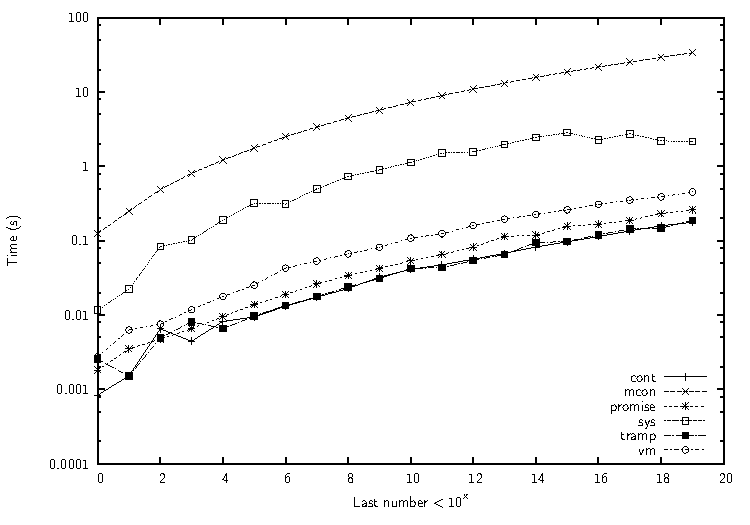
\includegraphics[width=\linewidth]{./kpn_exec_times_bw}
\caption{Bytecode}
\label{fig:kpn_exec_times_bc}
\end{subfigure}
\begin{subfigure}[b]{0.45\linewidth}
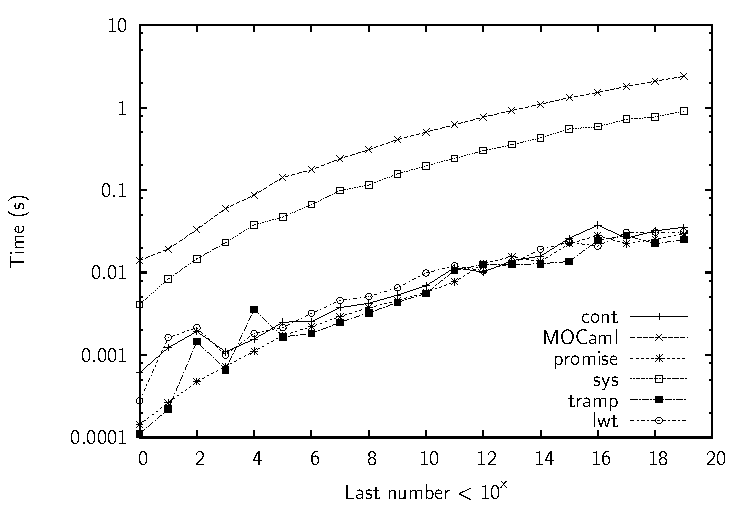
\includegraphics[width=\linewidth]{./kpn_exec_times_opt_bw}
\caption{Native code}
\label{fig:kpn_exec_times_nat}
\end{subfigure}
\cprotect\caption{\verb|kpn| execution time}
\label{fig:kpn_exec_times}
\end{figure}



\subsubsection{Sieve of Eratosthenes}
The sieve of Eratosthenes is one of the simplest algorithms to find primes:
\begin{enumerate}
\item{Start with number 2 and have all numbers greater or equal to 2 not crossed out.}
\item{Take the lowest not crossed out number: it is a prime.}
\item{Cross out all numbers divisible by the prime just found.}
\item{Repeat from step 2.}
\end{enumerate}

This algorithm is implemented using a dynamic process network. Initially the network is made up of four types of processes:
\begin{enumerate}
\item{Integers: generates the infinite sequence of integers starting from 2}
\item{Sift: If a number $ p $ is read Sift puts $ p $ forward to the printer process and it creates a new process, Filter $ p $ and inserts it between the input of Sift and Sift itself in the flow of numbers as shown in \Cref{fig:sieve_process_outline}. }
\item{Filter $ p $ discards all numbers divisible by $ p $ and passes everything else on.}
\item{Print just prints all numbers consumed.}
\end{enumerate}

This problem is a good example of dynamic thread creation that most general purpose concurrency frameworks should support.


\begin{figure}
\begin{tikzpicture}[->,>=stealth',shorten >=1pt,auto,node distance=2cm,
  thick,main node/.style={circle,draw,
  font=\sffamily\Large\bfseries,minimum size=8mm}, mvar/.style={rectangle, draw, ,minimum size=3mm}]
  \node[main node] (I1) [label=below:{Integers}] {};
  \node[mvar] (M11) [right=0.5 of I1, label=below:{$\text{m}_1$}] {};
  \node[main node] (S1) [right=8 of M11, label=below:{Sift}] {};
  \node[mvar] (MS1) [right=0.5 of S1, label=below:{$\text{m}_s$}] {};
  \node[main node] (P1) [right=1 of MS1, label=below:{Print}] {};
 
  \node[main node] (I2) [below= of I1, label=below:{Integers}] {};
  \node[mvar] (M12) [below=2.5 of M11, label=below:{$\text{m}_1$}] {};
  \node[main node] (F2) [right=0.5 of M12, label=below:{Filter 2}] {};
  \node[mvar] (M22) [right=0.5 of F2, label=below:{$\text{m}_s$}] {};
  \node[main node] (S2) [below= of S1, label=below:{Sift}] {};
  \node[mvar] (MS2) [below=2.5 of MS1, label=below:{$\text{m}_s$}] {};
  \node[main node] (P2) [below= of P1, label=below:{Print}] {};
  \node[main node] (I3) [below= of I2, label=below:{Integers}] {};
    \node[mvar] (M13) [below=2.5 of M12, label=below:{$\text{m}_1$}] {};
    \node[main node] (F22) [right=0.5 of M13, label=below:{Filter 2}] {};
      \node[mvar] (M23) [right=0.5 of F22, label=below:{$\text{m}_2$}] {};
   \node[main node] (F5) [right=0.5 of M23, label=below:{Filter 3}] {};
     \node[mvar] (M33) [right=0.5 of F5, label=below:{$\text{m}_s$}] {};
    \node[main node] (S3) [below= of S2, label=below:{Sift}] {};
    \node[mvar] (MS3) [below=2.5 of MS2, label=below:{$\text{m}_s$}] {};
    \node[main node] (P3) [below= of P2, label=below:{Print}] {};
  %\node[mvar] (F3) [below of=F2, label=below:{$\text{FIFO}_3$}] {};
  %\node[mvar] (F5) [below of=F3, label=below:{$\text{FIFO}_5$}] {};
  %\node[main node] (T2) [right = 1 of F2, label=below:{$\times 2$}] {};
  %\node[main node] (T3) [right = 1 of F3,  label=below:{$\times 3$}] {};
  %\node[main node] (T5) [right = 1 of F5, label=below:{$\times 5$}] {};
  %\node[mvar] (M2) [right of=T2, label=below:{$\text{m}_2$}] {};
  %\node[mvar] (M3) [right of=T3, label=below:{$\text{m}_3$}] {};
  %\node[mvar] (M5) [right of=T5, label=below:{$\text{m}_5$}] {};
  %\node[main node] (Merge35) [below=0.5 of M3, xshift=2cm, label=below:{$\text{merge}_{35}$}] {};
  %\node[mvar] (M35) [right of=Merge35, label=below:{$\text{m}_{35}$}] {};
  %\node[main node] (Merge235) [below=0.5 of M2, xshift=6cm, label=below:{$\text{merge}_{235}$}] {};
   %\node[mvar] (M235) [right of=Merge235, label=below:{$\text{m}_{235}$}] {};
  %\node[main node] (P) [right of=M235, label=below:{P}] {};
%  \node[main node] (S) [right of=E] {S};
%  \node[main node] (F) [right of=S] {F};
%  \node[main node] (I) [right of=F] {I};

  \path[every node/.style={font=\sffamily\small,
  		fill=white,inner sep=1pt}]
  	% Right-hand-side arrows rendered from top to bottom to
  	% achieve proper rendering of labels over arrows.
    (I1) edge   (M11)
    (M11) edge   (S1)
    (S1) edge   (MS1)
    (MS1) edge   (P1)
    (I2) edge   (M12)
    (M12) edge   (F2)
    (F2) edge   (M22)
    (M22) edge   (S2)
    (S2) edge   (MS2)
         edge[dashed, bend right=40]   (F2)
    (MS2) edge   (P2)
    (I3) edge   (M13)
    (M13) edge   (F22)
    (F22) edge   (M23)
    (M23) edge   (F5)
    (F5) edge   (M33)
    (M33) edge (S3)
    (S3) edge   (MS3)
    	edge[dashed, bend right=40]   (F5)
    (MS3) edge   (P3);
  %  (Merge35) edge   (M35)
  %  (M2) edge [bend left=20]   (Merge235)
  %  (M35) edge [bend left=40]   (Merge235)
  %  (Merge235) edge   (M235)
  %  (M235) edge   (P)
  %  (P) edge [out=150, in=40] (F2)
  %  (P) edge [out=120, in=130]  (F3)
  %  (P) edge [out=-150, in=-40]  (F5);
\end{tikzpicture}
\cprotect\caption{\verb|sieve| process outline}
\label{fig:sieve_process_outline}
\end{figure}



\begin{figure}[h]
\centering
\begin{subfigure}[b]{0.45\linewidth}
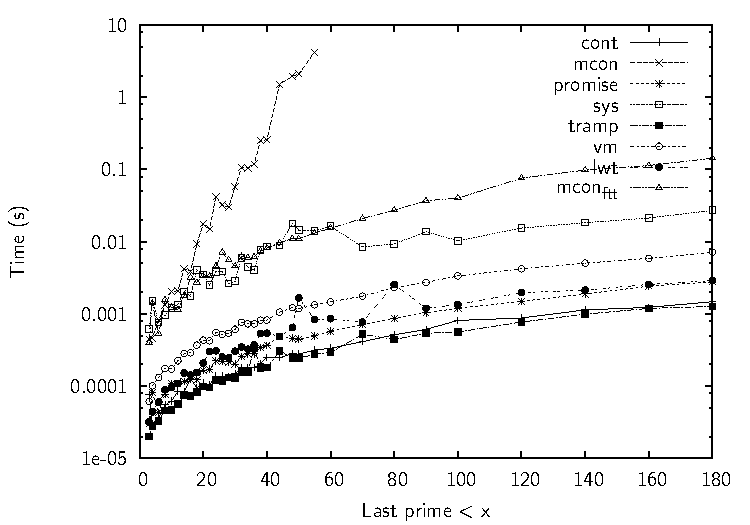
\includegraphics[width=\linewidth]{./sieve_exec_times_bw}
\caption{Bytecode}
\label{fig:sieve_exec_times_bc}
\end{subfigure}
\begin{subfigure}[b]{0.45\linewidth}
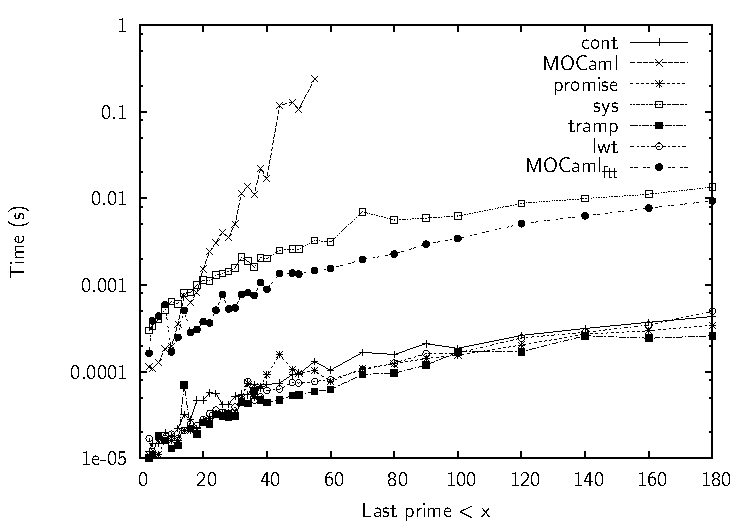
\includegraphics[width=\linewidth]{./sieve_exec_times_opt_bw}
\caption{Native code}
\label{fig:sieve_exec_times_nat}
\end{subfigure}
\cprotect\caption{\verb|sieve| execution time}
\label{fig:sieve_exec_times}
\end{figure}


Unlike the expectation, the concurrency framework with random reductions (mcon) in \Cref{fig:sieve_exec_times} exhibits an exponential behaviour. The reason for this is in the way random selection parameters relate to the \textbf{fork} tree formed by the expression.

Uniform random reductions assigns equal probabilities to each edge of a fork as it can be seen in \Cref{fig:sieve_without_ftt}. In general the probability that the filter process of the $ k $th prime fires is $ \frac{1}{2^{k+1}} $. This uneven probability distribution means that for the expected number of reduction steps taken by the system before finding the $ k $th prime is bigger than $ 2^{k+1} \in O(2^{k}) $ as it has to make at least one step within each filter.

However, the concurrency framework does not prescribe any evaluation strategy. It is possible to keep track of the fork tree at runtime and equalize the scheduling probabilities of all processes with every computation placeholder. This results in the scheduling probabilities shown in \Cref{fig:sieve_ftt}. These probabilities reduce the expected number of steps for the $ k $th prime to $ k(k+1) $. The speedup is easily seen on \Cref{fig:sieve_exec_times} with the series $ \text{mcon}_{\text{ftt}} $.

% Define styles for the different kind of edges in a Feynman diagram

\begin{figure}
\centering
\begin{subfigure}[b]{0.45\linewidth}
\begin{tikzpicture}[
        thick,
        % Set the overall layout of the tree
        level/.style={level distance=1.5cm},
        level 2/.style={sibling distance=2.6cm},
        level 3/.style={sibling distance=2cm}
    ]
    \coordinate
        % I have to insert a dummy child to get the tree to grow
        % correctly to the right.
        child[grow=right, level distance=0pt] {
        child  {
            child {
                node {output}
                edge from parent
                node [below] {$\frac{1}{4}$}
            }
            child {
                node {integers}
                edge from parent
                node [above] {$\frac{1}{4}$}
            }
            edge from parent
            node [below] {$\frac{1}{2}$}
        }
        child {
            child {
                node {filter2}
                edge from parent
                node [below] {$\frac{1}{4}$}
            }
            child {
                child {
                    node {filter3}
                    edge from parent
                    node [below] {$\frac{1}{8}$}
                }
                child {
                     child {
                         node {filter5}
                         edge from parent
                         node [below] {$\frac{1}{16}$}
                         }
                         child {
                          node {sift}
                          edge from parent
                          node [above] {$\frac{1}{16}$}
                         }
                    edge from parent
                    node [above] {$\frac{1}{8}$}
                }
                edge from parent
                node [above] {$\frac{1}{4}$}
            }
            edge from parent
            node [above] {$\frac{1}{2}$}
        }
    };
\end{tikzpicture}
\caption{Random without fork tree tracking}
\label{fig:sieve_without_ftt}
\end{subfigure}
\begin{subfigure}[b]{0.45\linewidth}
\begin{tikzpicture}[
        thick,
        % Set the overall layout of the tree
        level/.style={level distance=1.5cm},
        level 2/.style={sibling distance=2.6cm},
        level 3/.style={sibling distance=2cm}
    ]
    \coordinate
        % I have to insert a dummy child to get the tree to grow
        % correctly to the right.
        child[grow=left, level distance=0pt] {
        child  {
            child {
                node {output}
                edge from parent
                node [above] {$\frac{1}{6}$}
            }
            child {
                node {integers}
                edge from parent
                node [below] {$\frac{1}{6}$}
            }
            edge from parent
        }
        child {
            child {
                node {filter2}
                edge from parent
                node [above] {$\frac{1}{6}$}
            }
            child {
                child {
                    node {filter3}
                    edge from parent
                    node [above] {$\frac{1}{6}$}
                }
                child {
                     child {
                         node {filter5}
                         edge from parent
                         node [above] {$\frac{1}{6}$}
                         }
                         child {
                          node {sift}
                          edge from parent
                          node [below] {$\frac{1}{6}$}
                         }
                    edge from parent
                }
                edge from parent
            }
            edge from parent
        }
    };
\end{tikzpicture}
\caption{Fork tree tracking}
\label{fig:sieve_ftt}
\end{subfigure}
%

%\caption{Random without fork tree tacking
%
%

%\caption{Fork tree tracking}
%
\caption{Sieve fork tree}
\label{fig:sieve_fork_tree}
\end{figure}








\subsubsection{Concurrent sort}
The last example is concurrent sort. Sorting of a list of integers can be done by single comparator units as shown in \Cref{fig:sorter_process_single} which takes in two values and outputs the lower on one edge and the higher on the other. To sort an entire list we can arrange these elements in a network shown in \Cref{fig:sorter_process_full}. This network takes in the $ n $ element list $ x_0, x_1, \dots, x_n $ and outputs the result $ r_0, r_1, \dots, r_n $. For an $ n $ element list the network has $ \frac{n(n-1)}{2} $ nodes. Notice that bubble sort and insertion sort are two scheduling of this network. For simplicity I did not show the message variables in \Cref{fig:sorter_process_outline} but they are used on each arrow. This problem is a good example of a task best suited for lightweight concurrency: a very large number of simple threads statically allocated. For a list size of 500, there are 124750 threads. 

\begin{figure}
\centering

\begin{subfigure}[b]{0.45\linewidth}
\begin{tikzpicture}[->,>=stealth',auto,
  thick,main node/.style={circle,draw,
  font=\sffamily\Large\bfseries,minimum size=8mm}, mvar/.style={rectangle, draw, ,minimum size=3mm}]
  \node[main node] (I15) at (1,1) [] {};
  
  \node[] (INV1) at (-1,1) [] {x0};
  \node[] (INV2) at (1,3) [] {x1};
  \node[] (INV3) at (1,-1) [] {lo};
  \node[] (INV4) at (3,1) [] {hi};


  \path[every node/.style={font=\sffamily\small,
  		fill=white}]
     (INV1) edge (I15)
     (INV2) edge (I15)
     (I15) edge (INV3)
     (I15) edge (INV4);
  	% Right-hand-side arrows rendered from top to bottom to
  	% achieve proper rendering of labels over arrows.
   % (I1) edge   (M11)
    %(M11) edge   (S1)
   % (S1) edge   (MS1)
   % (MS1) edge   (P1);
  %  (Merge35) edge   (M35)
  %  (M2) edge [bend left=20]   (Merge235)
  %  (M35) edge [bend left=40]   (Merge235)
  %  (Merge235) edge   (M235)
  %  (M235) edge   (P)
  %  (P) edge [out=150, in=40] (F2)
  %  (P) edge [out=120, in=130]  (F3)
  %  (P) edge [out=-150, in=-40]  (F5);
\end{tikzpicture}
\caption{Single comparator}
\label{fig:sorter_process_single}
\end{subfigure}
\begin{subfigure}[b]{0.45\linewidth}
\begin{tikzpicture}[->,>=stealth',auto,
  thick,main node/.style={circle,draw,
  font=\sffamily\Large\bfseries,minimum size=8mm}, mvar/.style={rectangle, draw, ,minimum size=3mm}]
  \node[main node] (I15) at (1,5) [] {};
  \node[main node] (I14) at (1,4) [] {};
  \node[main node] (I24) at (2,4) [] {};
  \node[main node] (I13) at (1,3) [] {};
  \node[main node] (I23) at (2,3) [] {};
  \node[main node] (I33) at (3,3) [] {};
  \node[main node] (I12) at (1,2) [] {};
  \node[main node] (I22) at (2,2) [] {};
  \node[main node] (I32) at (3,2) [] {};
  \node[main node] (I42) at (4,2) [] {};
  \node[main node] (I11) at (1,1) [] {};
  \node[main node] (I21) at (2,1) [] {};
  \node[main node] (I31) at (3,1) [] {};
  \node[main node] (I41) at (4,1) [] {};
  \node[main node] (I51) at (5,1) [] {};
  
  \node[] (INV1) at (1,6) [] {};
  \node[] (INV2) at (-1,6) [] {x0};
  \node[] (INV3) at (-1,5) [] {x1};
  \node[] (INV4) at (-1,4) [] {x2};
  \node[] (INV5) at (-1,3) [] {x3};
  \node[] (INV6) at (-1,2) [] {x4};
  \node[] (INV7) at (-1,1) [] {x5};
  
  \node[] (INV8) at (6,1) [] {};
    \node[] (INV9) at (6,0) [] {r5};
    \node[] (INV10) at (5,0) [] {r4};
    \node[] (INV11) at (4,0) [] {r3};
    \node[] (INV12) at (3,0) [] {r2};
    \node[] (INV13) at (2,0) [] {r1};
    \node[] (INV14) at (1,0) [] {r0};
  
  
  %\node[mvar] (F3) [below of=F2, label=below:{$\text{FIFO}_3$}] {};
  %\node[mvar] (F5) [below of=F3, label=below:{$\text{FIFO}_5$}] {};
  %\node[main node] (T2) [right = 1 of F2, label=below:{$\times 2$}] {};
  %\node[main node] (T3) [right = 1 of F3,  label=below:{$\times 3$}] {};
  %\node[main node] (T5) [right = 1 of F5, label=below:{$\times 5$}] {};
  %\node[mvar] (M2) [right of=T2, label=below:{$\text{m}_2$}] {};
  %\node[mvar] (M3) [right of=T3, label=below:{$\text{m}_3$}] {};
  %\node[mvar] (M5) [right of=T5, label=below:{$\text{m}_5$}] {};
  %\node[main node] (Merge35) [below=0.5 of M3, xshift=2cm, label=below:{$\text{merge}_{35}$}] {};
  %\node[mvar] (M35) [right of=Merge35, label=below:{$\text{m}_{35}$}] {};
  %\node[main node] (Merge235) [below=0.5 of M2, xshift=6cm, label=below:{$\text{merge}_{235}$}] {};
   %\node[mvar] (M235) [right of=Merge235, label=below:{$\text{m}_{235}$}] {};
  %\node[main node] (P) [right of=M235, label=below:{P}] {};
%  \node[main node] (S) [right of=E] {S};
%  \node[main node] (F) [right of=S] {F};
%  \node[main node] (I) [right of=F] {I};

  \path[every node/.style={font=\sffamily\small,
  		fill=white}]
     (INV2) edge [-] (1,6)
     (1,6) edge (I15)
     (INV3) edge (I15)
     (INV4) edge (I14)
     (INV5) edge (I13)
     (INV6) edge (I12)
     (INV7) edge (I11)
     (I51) edge [-] (6,1)
     (I42) edge (I51)
     (I42) edge (I41)
     (I32) edge (I31)
     (I32) edge (I42)
     (I22) edge (I32)
     (I12) edge (I22)
     (I22) edge (I21)
     (I12) edge (I11)
     (I11) edge (I21)
     (I21) edge (I31)
     (I31) edge (I41)
     (I41) edge (I51)
     (I13) edge (I23)
     (I23) edge (I33)
     (I14) edge (I24)
     (I31) edge (I41)
     (I41) edge (I51)
     (I33) edge (I42)
     (I33) edge (I32)
     (I23) edge (I22)
     
     (I13) edge (I12)
     (I14) edge (I13)
     (I24) edge (I33)
     (I24) edge (I23)
     (I15) edge (I24)
     (I15) edge (I14)
     (6,1) edge (INV9)
     (I51) edge [-] (6,1)
     (I51) edge (INV10)
     (I41) edge (INV11)
     (I31) edge (INV12)
     (I21) edge (INV13)
     (I11) edge (INV14);
  	% Right-hand-side arrows rendered from top to bottom to
  	% achieve proper rendering of labels over arrows.
   % (I1) edge   (M11)
    %(M11) edge   (S1)
   % (S1) edge   (MS1)
   % (MS1) edge   (P1);
  %  (Merge35) edge   (M35)
  %  (M2) edge [bend left=20]   (Merge235)
  %  (M35) edge [bend left=40]   (Merge235)
  %  (Merge235) edge   (M235)
  %  (M235) edge   (P)
  %  (P) edge [out=150, in=40] (F2)
  %  (P) edge [out=120, in=130]  (F3)
  %  (P) edge [out=-150, in=-40]  (F5);
\end{tikzpicture}
\caption{Full sorting network}
\label{fig:sorter_process_full}
\end{subfigure}
\cprotect\caption{\verb|sorter| process outline}
\label{fig:sorter_process_outline}
\end{figure}

As expected, my system performed with the same characteristics as other lightweight concurrency solutions, but with a high overhead. Interestingly, the \textbf{vm} lightweight implementation shows very bad behaviour, however the heavyweight \textbf{sys} implementation performs better with lists longer than 250 elements. The memory use of my system is much higher than the other implementations as shown in \Cref{fig:sorter_mem}.


\begin{figure}[h]
\centering
\begin{subfigure}[b]{0.45\linewidth}
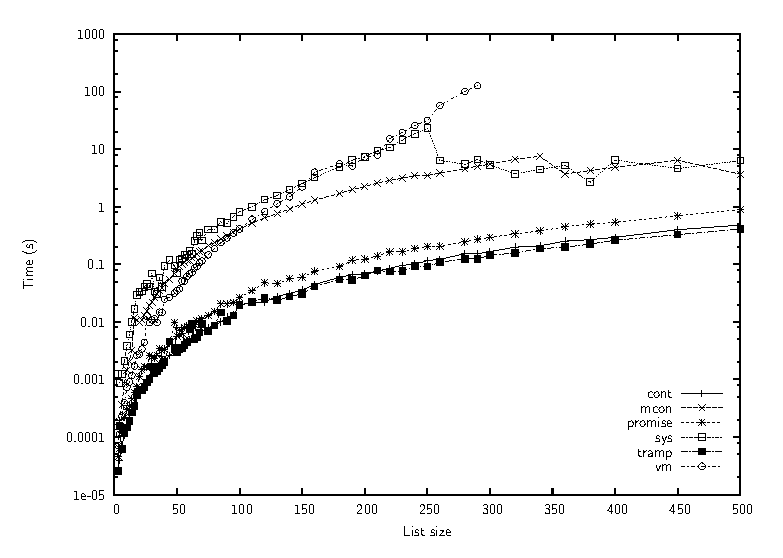
\includegraphics[width=\linewidth]{./sorter_exec_times_bw}
\caption{Bytecode}
\label{fig:sorter_exec_times_bc}
\end{subfigure}
\begin{subfigure}[b]{0.45\linewidth}
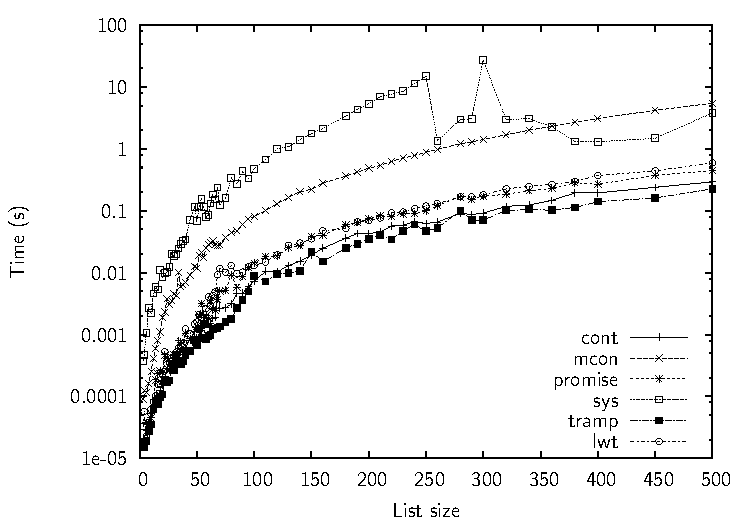
\includegraphics[width=\linewidth]{./sorter_exec_times_opt_bw}
\caption{Native code}
\label{fig:sorter_exec_times_nat}
\end{subfigure}
\cprotect\caption{\verb|sorter| execution time}
\label{fig:sorter_exec_times}
\end{figure}



\begin{figure}[h]
\centering
\begin{subfigure}[b]{0.45\linewidth}
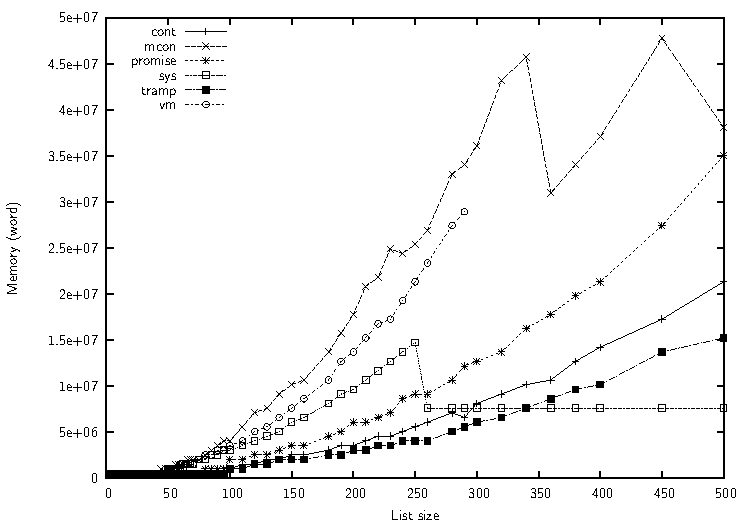
\includegraphics[width=\linewidth]{./sorter_mem_bw}
\caption{Bytecode}
\label{fig:sorter_mem_bc}
\end{subfigure}
\begin{subfigure}[b]{0.45\linewidth}
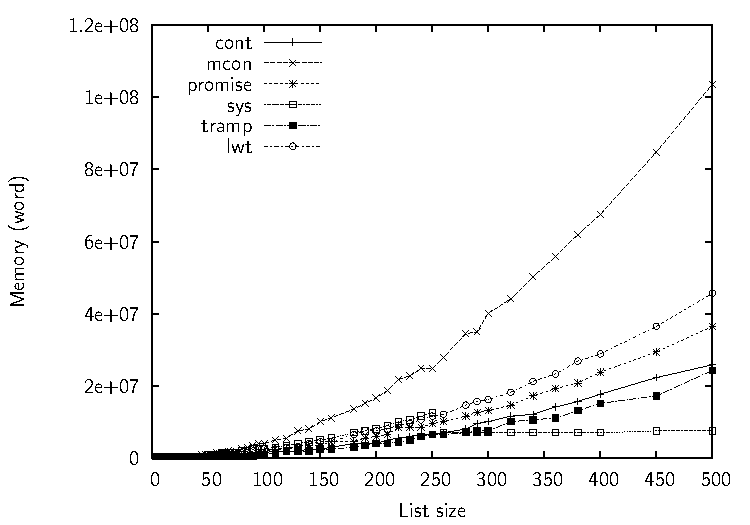
\includegraphics[width=\linewidth]{./sorter_mem_opt_bw}
\caption{Native code}
\label{fig:sorter_mem_nat}
\end{subfigure}
\cprotect\caption{\verb|sorter| memory use}
\label{fig:sorter_mem}
\end{figure}



\cleardoublepage
\chapter{Conclusion}

I hope that this rough guide to writing a dissertation is \LaTeX\ has
been helpful and saved you time.




\cleardoublepage

%%%%%%%%%%%%%%%%%%%%%%%%%%%%%%%%%%%%%%%%%%%%%%%%%%%%%%%%%%%%%%%%%%%%%
% the bibliography

\addcontentsline{toc}{chapter}{Bibliography}
\bibliography{refs}
\cleardoublepage

%%%%%%%%%%%%%%%%%%%%%%%%%%%%%%%%%%%%%%%%%%%%%%%%%%%%%%%%%%%%%%%%%%%%%
% the appendices
\appendix

\chapter{Full semantics}
\ottall
\label{chap:fullsemantics}

%\section{proposal.tex}
%{\scriptsize\verbatiminput{proposal.tex}}

%\section{propbody.tex}
%{\scriptsize\verbatiminput{propbody.tex}}



%\cleardoublepage

%\chapter{Makefile}

%\section{\label{makefile}Makefile}
%{\scriptsize\verbatiminput{makefile.txt}}

%\section{refs.bib}
%{\scriptsize\verbatiminput{refs.bib}}

\chapter{Coq definitions and theorem statements}
\label{cha:full_proof_statements}
\section{Weak bisimilarity definitions and theorems}
\begin{minipage}{\linewidth}
\begin{lstlisting}[language={Coq}, caption={Definitions of reduction relations}]
Inductive tauStep : relation expr :=
 | tStep :  forall (e e' : expr) (s : select), JO_red e s RL_tau e' -> tauStep e e'.

Definition tauRed : relation expr := (star tauStep).

Inductive totalDetTauStep : relation expr :=
 | ttStep : forall (e e' : expr),
   ( (tauStep e e') /\ 
   (forall (e'' : expr) (s : select) (l : label), JO_red e s (RL_labelled(l)) e'' -> False) /\ 
   (forall (e''' : expr), tauStep e e''' -> e' = e''')) -> totalDetTauStep e e'.
 
Definition totalTauRed : relation expr := (star totalDetTauStep).

Inductive labRed : label -> relation expr :=
 | lab_r : forall (e0 e1 e2 e3 : expr) (s : select) (l : label),
   tauRed e0 e1 /\
   JO_red e1 s (RL_labelled(l)) e2 /\
   tauRed e2 e3 -> labRed l e0 e3.
   
Inductive weakred : redlabel -> relation expr :=
 | weakred_T : forall ( e e' : expr ), tauRed e e' -> 
               weakred RL_tau e e'
 | weakred_L : forall ( e e' : expr) (l : label), labRed l e e' -> 
               weakred (RL_labelled l) e e'.               
\end{lstlisting}
\end{minipage}

\begin{minipage}{\linewidth}
\begin{lstlisting}[language={Coq}, caption={Definitions of weak bisimilarity}]
(* Milner *)
Definition isExprRelationWeakBisimilarity (R : relation expr) : Prop :=
   forall (p q : expr), R p q -> 
   ((forall (p' : expr) (l : label), 
     labRed l p p' ->
      (exists (q' : expr), labRed l q q' /\  R p' q' )) /\
    (forall (q' : expr) (l : label),
     labRed l q q' ->
      (exists (p' : expr), labRed l p p' /\  R p' q' )) /\ 
    (forall (p' : expr),
     tauRed p p' -> 
     (exists (q' : expr), tauRed q q' /\  R p' q' )) /\
    (forall (q' : expr), 
     tauRed q q' ->
      (exists (p' : expr), tauRed p p' /\  R p' q' ))
 ).

(* Sangiorgi *)
Definition isExprRelationStepWeakBisimilarity (R : relation expr) : Prop :=
   forall (p q : expr),
    R p q -> 
     ((forall (p' : expr) (rl : redlabel) (s: select),
        p [ s ] --> [ rl ] p' -> 
        (exists (q' : expr), weakred rl q q' /\  R p' q' )) /\
     (forall (q' : expr) (rl : redlabel) (s : select),
        q [ s ] --> [ rl ] q' ->
        (exists (p' : expr), weakred rl p p' /\  R p' q' ))).            
\end{lstlisting}
\end{minipage}

\begin{minipage}{\linewidth}
\begin{lstlisting}[language={Coq}, caption={Weak bisimilarity properties}]
Definition WBSM : relation expr -> Prop := isExprRelationStepWeakBisimilarity

Lemma isExprRelationWeakBisimilarity_equiv_WBSM : 
  forall (R : relation expr), 
   isExprRelationWeakBisimilarity R <-> WBSM R.

Lemma WBSM_comp : forall (R S : relation expr), WBSM R -> WBSM S -> WBSM (comp R S).

Lemma WBSM_eeq : forall (R S : relation expr), eeq R S -> WBSM R -> WBSM S.

Lemma WBSM_trans : forall (R : relation expr), WBSM R -> WBSM (trans R).

Lemma WBSM_star :forall (R : relation expr), WBSM R -> WBSM (star R).

Lemma WBSM_union2 : forall (R S : relation expr), WBSM R -> WBSM S -> WBSM (union2 R S).
\end{lstlisting}
\end{minipage}
\section{Monadic laws}
\section{Fork and join}
\begin{minipage}{\linewidth}
\begin{lstlisting}[language={Coq}, caption={Fork commutativity}]
Inductive fork_comm_rel :  relation expr := 
 | forkee_start : forall (e e' : expr), fork_comm_rel (e # e') (e' # e)
 | forkee_endl : forall (e e' : expr), is_value_of_expr e -> fork_comm_rel (e <# e') (e' #> e)
 | forkee_endr : forall (e e' : expr), is_value_of_expr e' -> fork_comm_rel (e #> e') (e' <# e).
 
Theorem fork_comm_wbsm: WBSM fork_comm_rel.
\end{lstlisting}
\end{minipage}
\section{Deadlock properties}
\section{Equivalence}
\cleardoublepage

\chapter{Project Proposal}



\section{Introduction of work to be undertaken}
With the rise of ubiquitous multiple core systems it is necessary for a working programmer to use concurrency to the greatest extent. However concurrent code has never been easy to write as human reasoning is often poorly equipped with the tools necessary to think about such systems. That is why it is essential for a programming language to provide safe and sound primitives to tackle this problem. 

My project aims to do this in the OCaml\cite{OCaml} language by developing a lightweight cooperating threading framework that holds correctness as a core value. The functional nature allows the use of one of the most recent trends in languages popular in academia, monads, to be used for a correct implementation. 

There have been two very successful frameworks, LWT\cite{LWT} and Async\cite{Async} that both provided the primitives for concurrent development in OCaml however neither is supported by a clear semantic description as their main focus was ease of use and speed. 
\section{Description of starting point}
My personal starting points are the courses ML under Windows (IA), Semantics of Programming Languages (IB), Logic and Proof (IB) and Concepts in Programming Languages (IB). Furthermore I have done extracurricular reading into semantics and typing and attended the Denotational Semantics (II) course in the past year.

The preparatory research period has to include familiarising myself with OCaml and the chosen specification and proof assistant tools.
\section{Substance and structure}
The project will consist of first creating a formal specification for a simple monad that has three main operations bind, return and choose. The behaviour of these operations will be specified in a current semantics tool like Lem\cite{Lem} or Ott\cite{Ott}. 

As large amount of research has gone into both monadic concurrency and implementations in OCaml, the project will draw inspiration from Claessen\cite{Claessen99functionalpearls}, Deleuze\cite{deleuzelight} and Vouillon\cite{vouillon2008lwt}.

Some atomic, blocking operations will also be specified including reading and writing to a console prompt or file to better illustrate the concurrency properties and make testing and evaluation possible.

This theory driven executable specification will be paired by a hand implementation and will be thoroughly checked against each other to ensure that both adhere to the desired semantics. 

Both of these implementations will be then compared against the two current frameworks for simplicity and speed on various test cases.

If time allows, an extension will also be carried out on the theorem prover version of the specification to formally verify that the implementation is correct. 
\section{Criteria}
For the project to be deemed a success the following items must be
successfully completed.
\begin{enumerate}
\item A specification for a monadic concurrency framework must be designed in the format of a semantics tool.
\item This specification needs to be exported to a proof assistant and has a runnable OCaml version
\item Test cases must be written that can thoroughly check a concurrency framework
\item A hand implementation needs to be designed, implemented and tested against the specification
\item The implementations must be compared to the frameworks LWT and Async based on speed
\item The dissertation must be planned and written
\end{enumerate}

In case the extension will also become viable then its success criterion is that there is a clear formal verification accompanying the automated theorem prover version of the specification.
\section{Timetable}
The project will be split into two week packages


\subsection{Week 1 and 2}
Preparatory reading and research into tools that can be used for writing the specification and in the extension, the proofs. The tools of choice at the time of proposal are Ott for the specification step and Coq\cite{Coq} as the proof assistant. Potentially a meeting arranged in the Computer Lab by an expert in using these tools. 

\textbf{Deliverable:} Small example specifications to try out the tool chain, including SKI combinator calculus.

\subsection{Week 3 and 4}
Investigating the two current libraries and their design decisions and planning the necessary parts of specification. Identifying the test cases that are thorough and common in concurrent code.

\textbf{Deliverable:} A document describing the major design decisions of the two libraries, the difference in design of the specification and a set of test cases much like the ones used in OCaml Light \cite{OCamlLight, OCamlLightWeb}, but with a concurrency focus.

\subsection{Week 5 and 6}
Writing the specification and exporting to automated theorem provers and OCaml.

\textbf{Deliverable:} The specification document in the format of the semantics tool and exported in the formats of the proof assistant and OCaml.


\subsection{Week 7 and 8}
Hand implement a version that adheres to the specification and test it against the runnable semantics.

\subsection{Week 9 and 10}
Evaluating the implementations of the concurrency framework against LWT and Async.
Writing up the halfway report.

\textbf{Deliverable:} Evaluation data and charts, the halfway report.
\subsection{Week 11 and 12}
If unexpected complexity occurs these two weeks can be used to compensate, otherwise starting on the verification proof in the proof assistant.
\subsection{Week 13 and 14}
If necessary adding more primitives (I/O, network) to test with, improving performance and finishing the verification proof. If time allows writing guide for future use of the framework.
\subsection{Week 15 and 16}
Combining all previously delivered documents as a starting point for the dissertation and doing any necessary further evaluation and extension.
Creating the first, rough draft of the dissertation.
\subsection{Week 17 and 18}
Getting to the final structure but not necessarily final wording of the dissertation, acquiring all necessary graphs and charts, incorporating ongoing feedback from the supervisor.
\subsection{Week 19 and 20}
Finalising the dissertation and incorporating all feedback and polishing. 
\section{Resource Declaration}
The project will need the following resources:
\begin{itemize}
\item MCS computer access that is provided for all projects
\item The OCaml core libraries and compiler
\item The LWT and Async libraries
\item The Lem tool
\item The Ott tool
\item The use of my personal laptop, to work more efficiently
\end{itemize}

As my personal laptop is included a suitable back-up plan is necessary which will consist of the following:
\begin{itemize}
\item A backup to my personal Dropbox account
\item A Git repository on Github
\item Frequent backups (potentially remotely) to the MCS partition
\end{itemize}
My supervisor and on request my overseers will receive access to both the Dropbox account and Github repository to allow full transparency.


\begin{thebibliography}{9}

\bibitem{OCaml}
 OCaml.
 \emph{http://ocaml.org/}

\bibitem{LWT}
 LWT, Lightweight Threading library.
 \emph{http://ocsigen.org/lwt/}

\bibitem{Async}
 Async, Open source concurrency library by Jane Street
 \emph{http://janestreet.github.io/}
 
 \bibitem{Lem}
 Lem, a tool for lightweight executable mathematics.\newline
 \emph{http://www.cs.kent.ac.uk/people/staff/sao/lem/}
 
 \bibitem{Ott}
  Ott, a tool for writing definitions of programming languages and calculi.
  Francesco Zappa Nardelli, Peter Sewell, and Scott Owens.\newline
 \emph{http://www.cl.cam.ac.uk/\textasciitilde pes20/ott/}

\bibitem{Claessen99functionalpearls}
  Claessen, Koen.
  \emph{Functional Pearls: A Poor Man's Concurrency Monad}.
  1999.

\bibitem{deleuzelight}
  Deleuze, Christophe.
  \emph{Light Weight Concurrency in OCaml: Continuations, Monads, Promises, Events}.

\bibitem{vouillon2008lwt}
  Vouillon, J{\'e}r{\^o}me.
  \emph{Lwt: a cooperative thread library} in Proceedings of the 2008 ACM SIGPLAN workshop on ML, pages 3--12.
  2008.
  ACM.
 
\bibitem{Coq}
 Coq proof assistant.
 \emph{http://coq.inria.fr/}

\bibitem{OCamlLight}  
 Owens, Scott.
 \emph{A sound semantics for OCaml light.} in Programming Languages and Systems, pages 1--15.
 2008.
 Springer Berlin Heidelberg.
 
\bibitem{OCamlLightWeb}
 Owens, Scott,
 \emph{http://www.cl.cam.ac.uk/\textasciitilde so294/ocaml/}.
 2008.
 


\end{thebibliography}



\end{document}
